\documentclass[10pt, letterpaper]{article}

% Inhaltsverzeichnis für Pakettypen (nur für Übersicht im Header, wird nicht im Dokument angezeigt)
% 1. Seitenlayout und Ränder
% 2. Sprache und Zeichensatz
% 3. Mathematik und Theorem-Umgebungen
% 4. Eigene Makros
% 5. Diagramme und Grafiken
% 6. Tabellen und Aufzählungen
% 7. Inhaltsverzeichnis
% 8. Abschnittsüberschriften
% 9. Abstrakt-Umgebung
% 10. Todos/Notizen
% 11. Rahmen/Box-Umgebungen
% 12. Python-Integration
% 13. Literaturverwaltung
% 14. Hyperlinks
% 15. Absatzeinstellungen
% 16. Umgebungen
% 17  Graphik
% 00. Titel und Autor

% --- 1. Seitenlayout und Ränder ---
\usepackage[margin=3cm]{geometry}

% --- 2. Sprache und Zeichensatz ---
\usepackage[english]{babel}
\usepackage[T1]{fontenc}
\usepackage[utf8]{inputenc}

% --- 3. Mathematik und Theorem-Umgebungen ---
\usepackage{amsmath, amssymb, amsthm}
\usepackage{mathrsfs}
\DeclareMathOperator{\WF}{WF}

% --- 4. Eigene Makros ---
\usepackage{xcolor}
\newcommand{\SKP}{\langle\cdot,\cdot\rangle}
\newcommand{\R}{\mathbb{R}}
\newcommand{\N}{\mathbb{N}}
\newcommand{\Q}{\mathbb{Q}}
\newcommand{\Z}{\mathbb{Z}}
\newcommand{\C}{\mathbb{C}}
\newcommand{\entwurf}[1]{\textcolor{red}{#1}}

% --- 5. Diagramme und Grafiken ---
\usepackage{graphicx}
\usepackage{tikz}
\usetikzlibrary{decorations.pathreplacing, arrows.meta, positioning}
\usepackage{tikz-cd}

% --- 6. Tabellen und Aufzählungen ---
\usepackage{enumitem}
\setlist[itemize]{left=0.5cm}

\newenvironment{romanenum}[1][]
  {%
    \ifx&#1&
    \else
      \textbf{#1}\quad
    \fi
    \begin{enumerate}[label=\roman*)]
  }
  {%
    \end{enumerate}%
  }

% --- 7. Inhaltsverzeichnis ---
\usepackage{tocloft}
\renewcommand{\cftsecfont}{\footnotesize}
\renewcommand{\cftsubsecfont}{\footnotesize}
\renewcommand{\cftsubsubsecfont}{\footnotesize}
\renewcommand{\cftsecpagefont}{\footnotesize}
\renewcommand{\cftsubsecpagefont}{\footnotesize}
\renewcommand{\cftsubsubsecpagefont}{\footnotesize}
\usepackage{etoc}

% --- 8. Abschnittsüberschriften ---
\usepackage{titlesec}
\titleformat{\section}{\normalfont\large\bfseries}{\thesection}{1em}{}
\titleformat{\subsection}{\normalfont\normalsize\bfseries}{\thesubsection}{0.5em}{}
\titleformat{\subsubsection}{\normalfont\normalsize\bfseries}{\thesubsubsection}{0.5em}{}
\setcounter{secnumdepth}{4}

% --- 9. Abstrakt-Umgebung ---
\usepackage{changepage}
\renewenvironment{abstract}
  {
    \begin{adjustwidth}{1.5cm}{1.5cm}
    \small
    \textsc{Abstract. –}%
  }
  {
    \end{adjustwidth}
  }

% --- 10. Todos/Notizen ---
\usepackage{todonotes}

% --- 11. Rahmen/Box-Umgebungen ---
\usepackage{mdframed}
\usepackage{tcolorbox}
\colorlet{shadecolor}{gray!25}

\newenvironment{customTheorem}
  {\vspace{10pt}%
   \begin{mdframed}[
     backgroundcolor=gray!20,
     linewidth=0pt,
     innertopmargin=10pt,
     innerbottommargin=10pt,
     skipabove=\dimexpr\topsep+\ht\strutbox\relax,
     skipbelow=\topsep,
   ]}
  {\end{mdframed}
   \vspace{10pt}%
  }

% --- 12. Python-Integration ---
% (Deaktiviert in dieser Version, aktiviere bei Bedarf)
% \usepackage{pythontex}
% \usepackage[makestderr]{pythontex}

% --- 13. Literaturverwaltung ---
\usepackage{csquotes}
\usepackage[backend=biber, style=alphabetic, citestyle=alphabetic]{biblatex}
\addbibresource{bibliography.bib}

% --- 14. Hyperlinks ---
\usepackage{hyperref}
\hypersetup{
  colorlinks   = true,
  urlcolor     = blue,
  linkcolor    = blue,
  citecolor    = blue,
  frenchlinks  = true
}

% --- 15. Absatzeinstellungen ---
\usepackage[parfill]{parskip}
\sloppy

% --- 16. Umgebungen ---
\usepackage{thmtools}

\newcommand{\CustomHeading}[3]{%
  \par\medskip\noindent%
  \textbf{#1 #2} \textnormal{(#3)}.\enskip%
}

\newenvironment{DEF}[2]{\CustomHeading{Definition}{#1}{#2}}{}
\newenvironment{PROP}[2]{\CustomHeading{Proposition}{#1}{#2}}{}
\newenvironment{THEO}[2]{\CustomHeading{Theorem}{#1}{#2}}{}
\newenvironment{LEM}[2]{\CustomHeading{Lemma}{#1}{#2}}{}
\newenvironment{KORO}[2]{\CustomHeading{Corollar}{#1}{#2}}{}
\newenvironment{REM}[2]{\CustomHeading{Remark}{#1}{#2}}{}
\newenvironment{EXA}[2]{\CustomHeading{Example}{#1}{#2}}{}
\newenvironment{STUD}[2]{\CustomHeading{Study}{#1}{#2}}{}
\newenvironment{CONC}[2]{\CustomHeading{Concept}{#1}{#2}}{}

\newenvironment{PROOF}
  {\begin{proof}}%
{\end{proof}}

% --- Unit Umgebung für Source-Inhalte ---
\usepackage{mdframed}
\newmdenv[
  linewidth=1pt,
  topline=false,
  bottomline=false,
  rightline=false,
  leftmargin=0cm,
  rightmargin=0cm,
  skipabove=10pt,
  skipbelow=10pt,
  innertopmargin=0.5\baselineskip,
  innerbottommargin=0.5\baselineskip,
  backgroundcolor=gray!10,
  linecolor=gray
]{unitbox}

\newenvironment{unit}[1]
  {\begin{unitbox}\textbf{Unit #1}\par\smallskip}
  {\end{unitbox}}

% --- 17. Graphik ---
\usepackage{graphicx}
\graphicspath{ {./images/} }
\usepackage[export]{adjustbox}




\usepackage{cancel}


% --- 00. Titel und Autor ---
\title{Mein Titel}
\author{Tim Jaschik}
\date{\today}


%New command to display footnote whose markers will always be hidden
\let\svthefootnote\thefootnote
\newcommand\blfootnotetext[1]{%
  \let\thefootnote\relax\footnote{#1}%
  \addtocounter{footnote}{-1}%
  \let\thefootnote\svthefootnote%
}

%Overriding the \footnotetext command to hide the marker if its value is `0`
\let\svfootnotetext\footnotetext
\renewcommand\footnotetext[2][?]{%
  \if\relax#1\relax%
    \ifnum\value{footnote}=0\blfootnotetext{#2}\else\svfootnotetext{#2}\fi%
  \else%
    \if?#1\ifnum\value{footnote}=0\blfootnotetext{#2}\else\svfootnotetext{#2}\fi%
    \else\svfootnotetext[#1]{#2}\fi%
  \fi
}


\begin{document}

\maketitle
\rule{\textwidth}{0.5pt}
\begin{abstract}
Kurze Beschreibung …
\end{abstract}
\rule{\textwidth}{0.5pt}
\vspace{0.5cm}

\tableofcontents

\pagebreak


with the complexification of the tangent bundle. In order to relate the PIC condition to the $1 / 4$-pinching sphere theorem, we present the argument of Brendle and Schoen [BS09a] that relates the $1 / 4$-pinching condition with the PIC condition on $M \times \mathbb{R}^{2}$. The result, i.e. Corollary 14.13, shows that $M$ is a compact manifold with pointwise $1 / 4$-pinched sectional curvature, then $M \times \mathbb{R}^{2}$ has positive isotropic curvature.

Chapter 14 brings the discussion to a climax. Here we finally give a proof of the differentiable $1 / 4$-pinching sphere theorem from the material presented in earlier chapters. In the final section we outline a general convergence result due to Brendle [Bre08] which looks at the weaker condition of PIC on $M \times \mathbb{R}$.

A synopsis of the chapter progressions and inter-relationships is summarised by the following diagram:\\
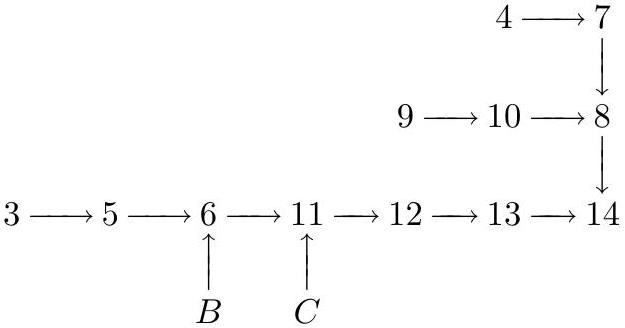
\includegraphics[scale=0.3, center]{2025_05_21_2f79b74cab2419f5632dg-011}

Here the main argument is represented along the horizontal together with the supplementary appendices. The regularity, existence theory and blow-up analysis are shown above this.

This book grew from my honours thesis completed in 2008 at the Australian National University. I would like to express my deepest gratitudes to my supervisor, Dr Ben Andrews, for without his supervision, assistance and immeasurable input this book would not be possible. Finally, I would like to thank my parents for their continuous support and encouragement over the years.



\pagebreak

\section*{Notation and List of Symbols}


\begin{center}
\begin{tabular}{|l|l|}
\hline
$\Gamma_{i j}^{k}$ & Christoffel symbol of a connection $\nabla$ w.r.t. a local frame ( $\partial_{i}$ ). \\
\hline
( $x^{i}$ ) & A local coordinate chart for a neighbourhood $U$ with a local chart $x=\left(x^{i}\right): U \rightarrow \mathbb{R}^{n}$. \\
\hline
Curv & Algebraic curvature operators. \\
\hline
$I$, id & The identities on $S^{2}\left(\bigwedge^{2} V^{*}\right)$ and $S^{2}(V)$. N.B. $I=\mathrm{id} \wedge \mathrm{id}$. \\
\hline
inj & Injectivity radius. \\
\hline
$\Delta_{g, h}$ & Harmonic map Laplacian w.r.t. the domain metric $g$ and codomain metric $h$. \\
\hline
$\wedge^{2} V$ & Second exterior power of the vector space $V$. \\
\hline
$\mathcal{L}_{X}$ & Lie derivative w.r.t. the vector field $X$. \\
\hline
Met & Space of metrics. \\
\hline
$\mathcal{N}_{x} A$ & Normal cone to $A$ at $x$. \\
\hline
$\nu$ & Unit outward normal. \\
\hline
(1) & Kulkarni-Nomizu product. \\
\hline
${ }^{f} \nabla$ & Pullback connection on $f^{*} E$. \\
\hline
$f^{*} E$ & Pullback bundle of E by f. \\
\hline
$\xi_{f},\left(\xi_{i}\right)_{f}$ & Restriction of $\xi, \xi_{i} \in \Gamma(E)$ to $f$. \\
\hline
$R, R_{i j k \ell}$ & Riemannian curvature tensor. \\
\hline
Ric, $R_{i j}$ & Ricci curvature tensor. \\
\hline
Scal & Scalar curvature tensor. \\
\hline
$\Gamma(E)$ & The space of smooth sections of a vector bundle $\pi: E \rightarrow M$. \\
\hline
$\mathfrak{S}$ & Spatial tangent bundle. \\
\hline
$\operatorname{Sym}^{2} T^{*} M$ & Symmetric (2, 0)-bundle over M. \\
\hline
$S^{2}(U)$ & Symmetric tensor space of $U$. \\
\hline
$T_{\ell}^{k}(V)$ & The set of all multilinear maps $\left(V^{*}\right)^{\ell} \times V^{k} \rightarrow \mathbb{R}$ over $V$. \\
\hline
$T_{\ell}^{k} M$ & ( $k, \ell$ )-tensor bundle over a manifold $M$. \\
\hline
$\mathscr{T}_{\ell}{ }^{k}(M)$ & The space of ( $k, \ell$ )-tensor fields over $M$, i.e. $\Gamma\left(\otimes^{k} T^{*} M \otimes^{\ell} T M\right)$. \\
\hline
$\mathcal{T}_{x} A$ & Tangent cone to $A$ at $x$. \\
\hline
$d \mu, d \mu(g)$ & Volume form with respect to a metric $g$. \\
\hline
$d \sigma$ & Volume form on a hypersurface or boundary of a manifold. \\
\hline
$\mathscr{X}(M)$ & The space of vector fields, i.e. $\Gamma(T M)$. \\
\hline
\end{tabular}
\end{center}




\pagebreak

\section{Chapter 1 Introduction}
The relationship between curvature and topology has traditionally been one of the most popular and highly developed topics in Riemannian geometry. In this area, a central issue of concern is that of determining global topological structures from local metric properties. Of particular interest to us the socalled pinching problem and related sphere theorems in geometry. We begin with a brief overview of this problem, from Hopf's inspiration to the latest developments in Hamilton's Ricci flow.

\subsection*{Manifolds with Constant Sectional Curvature}
One of the earliest insights into the relationship between curvature and topology is the problem of classifying complete Riemannian manifolds with constant sectional curvature, referred to as space forms. In the late 1920s Heinz Hopf studied the global properties of such space forms and proved, in his PhD dissertation [Hop25] (see also [Hop26]), the following:

Theorem 1.1 (Uniqueness of Constant Curvature Metrics). Let M be a complete, simply-connected, $n$-dimensional Riemannian manifold with constant sectional curvature. Then $M$ is isometric to either $\mathbb{R}^{n}, S^{n}$ or $\mathbb{H}^{n}$.

Furthermore, if the manifold is compact then the space forms are compact quotients of the either $\mathbb{R}^{n}, S^{n}$ or $\mathbb{H}^{n}$. Placing this result on solid ground was one of Hopf's tasks during the 1930s, however the classification is still incomplete (the categorisation of hyperbolic space quotients has been extremely problematic).

Given these developments, curiosity permits one to ask if a similar result would hold under a relaxation of the curvature hypothesis. In other words, assuming a compact manifold has a sectional curvature 'varying not too much' (we will later say the manifold is 'pinched'), can one deduce that the underlying manifold is topologically (one would even hope differentiably) identical to one of the above space forms? After rescaling the metric there are three\\
cases: the pinching problem around $\kappa_{0}=+1,0,-1$. Therefore if the sectional curvature $K$ satisfies $\left|K-\kappa_{0}\right| \leq \varepsilon$, the question becomes one of finding an optimal $\varepsilon>0$ in which the manifold is identical (in some sense) to a particular space form.

For our purposes, the question of interest is that of positive pinching around $\kappa_{0}=1$; our subsequent discussion will focus entirely on this case. The problem has enjoyed a great deal interest over the years due to its historical importance both in triggering new results and as motivation for creating new mathematical tools.

\subsection*{The Topological Sphere Theorem}
The only simply connected manifold of constant positive sectional curvature is, by the above theorem, the sphere. A heuristic sense of continuity leads one to hope that if the sectional curvature of a manifold is close to a positive constant, then the underlying manifold will still be a sphere. Hopf himself repeatedly put forward this problem, in particular when Harry Rauch (an analyst and expert in Riemannian surfaces) visited him in Zürich throughout 1948-1949. Rauch was so enthusiastic about Hopf's pinching that, back at the Institute for Advanced Study in Princeton, he finally managed to prove Hopf's conjecture with a pinching constant of roughly $\delta \approx 3 / 4$. Specifically Rauch [Rau51] proved:

Theorem 1.2 (Rauch, 1951). Let ( $M^{n}, g$ ) be a complete Riemannian manifold with $n \geq 2$. If the sectional curvature $K(p, \Pi)$ (where $p \in M$ and $\Pi$ is a 2-dimensional plane through p) satisfies

$$
\delta k \leq K(p, \Pi) \leq k-\varepsilon
$$

for some constant $k>0$, some $\varepsilon>0$, all $p \in M$; and all planes $\Pi$, where $\delta \approx 3 / 4$ is the root of the equation $\sin \pi \sqrt{\delta}=\sqrt{\delta} / 2$. Then the simply connected covering space of $M$ is homeomorphic to the $n$-dimensional sphere $S^{n}$. In particular if $M$ is simply connected, then $M$ is homeomorphic to $S^{n}$.

Rauch's paper is seminal in two respects. First of all, he was able to control the metric on both sides. Secondly, to get a global result, he made a subtle geometric study in which he proved that (under the pinching assumption) one can build a covering of the manifold from the sphere.

Thereafter Klingenberg [Kli59] sharpened the constant - in the even dimensional case - to the solution of $\sin \pi \sqrt{\delta}=\sqrt{\delta}$ (i.e. $\delta \approx 0.54$ ). Crucially, the precise notion of an injectivity radius was introduced to the pinching problem. Using this, Berger [Ber60a] improved Klingenberg's result, under the even dimension assumption, with $\delta=1 / 4$. Finally, Klingenberg [Kli61] extended the\\
injectivity radius lower estimate to odd dimensions. This proved the sphere theorem in its entirely. The resulting quarter pinched sphere theorem is stated as follows:

Theorem 1.3 (Rauch-Klingenberg-Berger Sphere Theorem). If $a$ simply connected, complete Riemannian manifold has sectional curvature $K$ satisfying

$$
\frac{1}{4}<K \leq 1
$$

then it is homeomorphic to a sphere. ${ }^{1}$\\
The theorem's pinching constant is optimal since the conclusion is false if the inequality is no longer strict. The standard counterexample is complex projective space with the Fubini-Study metric (sectional curvatures of this metric take on values between $1 / 4$ and 1 inclusive). Other counterexamples may be found among the rank one symmetric spaces (see e.g. [Hel62]).

As a matter of convention, we say a manifold is strictly $\delta$-pinched in the global sense if $0<\delta<K \leq 1$ and weakly $\delta$-pinched in the global sense if $0<\delta \leq K \leq 1$. In which case the sphere theorem can be reformulated as: 'Any complete, simply-connected, strictly $1 / 4$-pinched Riemannian manifold is homeomorphic to the sphere.'

\subsubsection*{Remarks on the Classical Proof}
The proof from the 1960s consisted in arguing that the manifold can be covered with only two topological balls (e.g. see [AM97, Sect. 1]). The proof relies heavily on classical comparison techniques.\\
Idea of Proof. Choose points $p$ and $q$ in such a way that the distance $d(p, q)$ is maximal, that is $d(p, q)=\operatorname{diam}(M)$. The key property of such a pair of points is that for any unit tangent vector $v \in T_{q} M$, there exists a minimising geodesic $\gamma$ from $q$ to $p$ making an acute angle with $v$. From this one can apply Toponogov's triangle comparison theorem [Top58] (see also [CE08, Chap. 2]) and Klingenberg's injectivity radius estimates to show that

$$
M=B(p, r) \cup B(q, r)
$$

\footnotetext{${ }^{1}$ In the literature some quote the sectional curvature as taking values in the interval $(1,4]$. This is only a matter of scaling. For instance, if the metric is scaled by a factor $\lambda$ then the sectional curvatures are scaled by $1 / \lambda$. Thus one can adjust the maximum principal curvature to 1 , say. What is important about the condition is that the ratio of minimum to maximum curvature remains greater than $1 / 4$.
}
for $\pi / 2 \sqrt{\delta}<r<\pi$ and $1 / 4<\delta \leq K \leq 1$. In other words, under the hypothesis of the sphere theorem, we can write $M$ as a union of two balls. One then concludes, by classical topological arguments, that $M$ is homeomorphic to the sphere.

\subsubsection*{Manifolds with Positive Isotropic Curvature}
One cannot overlook the contributions made by Micallef and Moore [MM88] in generalising the classical Rauch-Klingenberg-Berger sphere theorem. By introducing the so-called positive isotropic curvature condition to the problem together with harmonic map theory, they managed to prove the following:\\
Theorem 1.4 (Micallef and Moore, 1988). Let $M$ be a compact simply connected $n$-dimensional Riemannian manifold which has positive curvature on totally isotropic 2-planes, where $n \geq 4$. Then $M$ is homeomorphic to a sphere.

This is achieved as follows: Firstly, for a $n$-dimensional Riemannian manifold $M$ with positive curvature on totally isotropic two-planes one can show that any nonconstant conformal harmonic map $f: S^{2} \rightarrow M$ has index at least $\frac{n-3}{2}$. The proof uses classical results of Grothendieck on the decomposition of holomorphic bundles over $S^{2}$. Secondly, one can show: If $M$ is a compact Riemannian manifold such that $\pi_{k}(M) \neq 0$, where $k \geq 2$, then there exists a nonconstant harmonic 2 -sphere in $M$ of index $\leq k-2$. This fact is a modification of the Sacks-Uhlenbeck theory of minimal 2-spheres in Riemannian manifolds. From this, the above theorem easily follows by using duality with these two results, and using the higher-dimensional Poincaré conjecture, which was proved for $n \geq 5$ by Smale and for $n=4$ by Freedman.

A refined version of the classical sphere theorem now follows by replacing the global pinching hypotheses on the curvature by a pointwise one. In particular we say that a manifold $M$ is strictly $\delta$-pinched in the pointwise sense if $0<\delta K\left(\Pi_{1}\right)<K\left(\Pi_{2}\right)$ for all points $p \in M$ and all 2-planes $\Pi_{1}, \Pi_{2} \subset T_{p} M$. Furthermore, we say $M$ is weakly $\delta$-pinched in the pointwise sense if $0 \leq \delta K\left(\Pi_{1}\right) \leq K\left(\Pi_{2}\right)$ for all point $p \in M$ and all 2-planes $\Pi_{1}, \Pi_{2} \subset T_{p} M$. In which case it follows from Berger's Lemma (see Sect. 2.7.7) that any manifold which is strictly $1 / 4$-pinched in the pointwise sense has positive isotropic curvature (and so is homeomorphic to $S^{n}$ ).

\subsubsection*{A Question of Optimality}
Given the above stated Rauch-Klingenberg-Berger sphere theorem, a natural question to ask is: Can the homeomorphic condition can be replaced by a diffeomorphic one? In answering this, there are some dramatic provisos.

The biggest concerns the method used in the above classical proof - as the argument presents $M$ as a union of two balls glued along their common boundary so that $M$ is homeomorphic to $S^{n}$. However, Milnor [Mil56] famously showed that there are 'exotic' structures on $S^{7}$, namely:\\
Theorem 1.5 (Milnor, 1956). There are 7-manifolds that are homeomorphic to, but not diffeomorphic to, the 7-sphere. ${ }^{2}$\\
Moreover, some exotic spheres are precisely obtained by gluing two half spheres along their equator with a weird identification. Hence the above classical proof cannot do better since it does not allow one to obtain a diffeomorphism between $M$ and $S^{n}$ in general. As a result, it remained an open question as to whether or not the sphere theorem's conclusion was optimal in this sense.

To add to matters, it has also been a long-standing open problem as to whether there actually are any concrete examples of exotic spheres with positive curvature. This has now apparently been resolved by Petersen and Wilhelm [PW08] who show there is a metric on the Gromoll-Meyer Sphere with positive sectional curvature.

\subsection*{The Differentiable Sphere Theorem}
There have been many attempts at proving the differentiable version, most of which have been under sub-optimal pinching assumptions. The first attempt was by Gromoll [Gro66] with a pinching constant $\delta=\delta(n)$ that depended on the dimension $n$ and converged to 1 as $n$ goes to infinity. The result for $\delta$ independent of $n$ was obtained by Sugimoto, Shiohama, and Karcher [SSK71] with $\delta=0.87$. The pinching constant was subsequently improved by Ruh [Ruh71,Ruh73] with $\delta=0.80$ and by Grove, Karcher and Ruh [GKR74] with $\delta=0.76$. Furthermore, Ruh [Ruh82] proved the differentiable sphere theorem under a pointwise pinching condition with a pinching constant converging to 1 as $n \rightarrow \infty$.

\subsubsection*{The Ricci Flow}
In 1982 Hamilton introduced fundamental new ideas to the differentiable pinching problem. His seminal work [Ham82b] studied the evolution of a heat-type geometric evolution equation:

$$
\frac{\partial}{\partial t} g(t)=-2 \operatorname{Ric}(g(t)) \quad g(0)=g_{0}
$$

\footnotetext{${ }^{2}$ In fact Milnor and Kervaire [KM63] showed that $S^{7}$ has exactly 28 nondiffeomorphic smooth structures.
}
herein referred to as the Ricci flow. This intrinsic geometric flow has, over the years, served to be an invaluable tool in obtaining global results within the differentiable category. The first of which is following result due to Hamilton [Ham82b].

Theorem 1.6 (Hamilton, 1982). Suppose $M$ is a simply-connected compact Riemannian 3-manifold with strictly positive Ricci curvature. Then M is diffeomorphic to $S^{3}$.

Following this, Hamilton [Ham86] developed powerful techniques to analyse the global behaviour of the Ricci flow. This enabled him to extend his previous result to 4 -manifolds by showing:

Theorem 1.7 (Hamilton, 1986). A compact 4-manifold $M$ with a positive curvature operator is diffeomorphic to the sphere $S^{4}$ or the real projective space $\mathbb{R} P^{4}$.

Note that we say a manifold has a positive curvature operator if the eigenvalues if $R$ are all positive, or alternatively $R(\phi, \phi)>0$ for all 2-forms $\phi \neq 0$ (when considering the curvature operator as a self-adjoint operator on two-forms).

Following this, Chen [Che91] show that the conclusion of Hamilton's holds under the weaker assumption that the manifold has a 2-positive curvature operator. Specifically, he proved that: If $M$ is a compact 4-manifold with a 2-positive curvature operator, then $M$ is diffeomorphic to either $S^{4}$ or $\mathbb{R} P^{4}$. Moreover, Chen showed that the 2 -positive curvature condition is implied by pointwise $1 / 4$-pinching. In which case he managed to show:

Theorem 1.8 (Chen, 1991). If $M^{4}$ is a compact pointwise $1 / 4$-pinched 4-manifold, then $M$ is either diffeomorphic to the sphere $S^{4}$ or the real projective space $\mathbb{R} P^{4}$, or isometric to the complex projective space $\mathbb{C} P^{2}$.

Note that we say a manifold has a 2-positive curvature operator if the sum of the first two eigenvalues of $R$ are positive. ${ }^{3}$ It is easy to see that when $\operatorname{dim} M=3$, the condition of positive Ricci and 2-positive curvature operator are equivalent (in fact, 2-positive implies positive Ricci in n-dimensions).

However despite this progress it still remained an open problem for over a decade as to whether or not these results could be extended for manifolds $M$ with $\operatorname{dim} M \geq 4$.

\footnotetext{${ }^{3}$ Equivalently one could also say that $R(\phi, \phi)+R(\psi, \psi)>0$ for all 2-forms $\phi$ and $\psi$ satisfying $|\phi|^{2}=|\psi|^{2}$ and $\langle\phi, \psi\rangle=0$.
}\subsubsection*{Ricci Flow in Higher Dimensions}
Huisken [Hui85] was one of the first to study the Ricci flow on manifolds of dimension $n \geq 4$. His analysis focuses on decomposing the curvature tensor into $R_{i j k \ell}=U_{i j k \ell}+V_{i j k \ell}+W_{i j k \ell}$, where $U_{i j k \ell}$ denotes the part of the curvature tensor associated with the scalar curvature, $V_{i j k \ell}$ is the part of the curvature associated with the trace-free Ricci curvature, and $W_{i j k \ell}$ denotes the Weyl tensor. By following the techniques outlined in [Ham82b], Huisken showed that if the scalar-curvature-free part of the sectional curvature tensor is small compared to the scalar curvature, then the same evolution equation for the curvature yields the same result - a deformation to a constant positive sectional curvature metric.

Theorem 1.9 (Huisken, 1985). Let $n \geq 4$. If the curvature tensor of a smooth compact $n$-dimensional Riemannian manifold of positive scalar curvature satisfies

$$
|W|^{2}+|V|^{2}<\delta_{n}|U|^{2}
$$

with $\delta_{4}=\frac{1}{5}, \delta_{5}=\frac{1}{10}$, and $\delta_{n}=\frac{2}{(n-2)(n+1)}$ for $n \geq 6$, then the Ricci flow has a solution $g(t)$ for all times $0 \leq t<\infty$ and $g(t)$ converges to a smooth metric of constant positive curvature in the $C^{\infty}$-topology as $t \rightarrow \infty$.

There are also similar results by Nishikawa [Nis86] and Margerin [Mar86] with more recent sharp results by Margerin [Mar94a, Mar94b] as well.

In 2006, Böhm and Wilking [BW08] managed to generalise Chen's work in four dimensions by constructed a new family of cones (in the space of algebraic curvature operators) which is invariant under Ricci flow. This allowed them to prove:

Theorem 1.10 (Böhm and Wilking, 2006). On a compact manifold $M^{n}$ the Ricci flow evolves a Riemannian metric with 2-positive curvature operator to a limit metric with constant sectional curvature.

Their paper [BW08] overcomes some major technical problems, particular those related to controlling the Weyl part of the curvature.

Soon thereafter, Brendle and Schoen [BS09a] finally managed to prove:\\
Theorem 1.11 (Brendle and Schoen, 2007). Let $M$ be a compact Riemannian manifold of dimension $n \geq 4$ with sectional curvature strictly $1 / 4$-pinched in the pointwise sense. Then $M$ admits a metric of constant curvature and therefore is diffeomorphic to a spherical space form.

The key novel step in the proof is to show that nonnegative isotropic curvature is invariant under the Ricci flow. This was also independently proved by Nguyen [Ngu08, Ngu10]. Brendle and Schoen obtain the abovementioned result by working with the nonnegative isotropic curvature condition on\\
$M \times \mathbb{R}^{2}$, which is implied by pointwise $1 / 4$-pinching. We will examine this proof by Brendle and Schoen [BS09a] in Chap. 14. In Chaps. 12 and 13 we will look at the methods of Böhm and Wilking [BW08] in detail with the specific aim to proving the differentiable pointwise $1 / 4$-pinching sphere theorem for $n \geq 4$.

Finally, in Chap. 15 we survey the following result of Brendle [Bre08] which generalises the earlier results of [Ham82b, Hui85, Che91, BW08, BS09a].

Theorem 1.12 (Brendle, 2008). Let ( $M, g_{0}$ ) be a compact Riemannian manifold of dimension $n \geq 4$ such that $M \times \mathbb{R}$ has positive isotropic curvature. Then there is a unique maximal solution $g(t), t \in[0, T)$ to the Ricci flow with initial metric $g_{0}$ which converges to a metric of constant curvature. In particular, $M$ is diffeomorphic to a spherical space form.

\subsection*{Where to Next?}
There is a big problem crying out for an application of Ricci flow:

\begin{displayquote}
If $\left(M, g_{0}\right)$ is a simply connected compact Riemannian manifold with positive curvature on isotropic 2-planes, is $M$ diffeomorphic to a spherical space form? ${ }^{4}$
\end{displayquote}

The difficulties are manifold: First, it is very difficult to bring in the condition of simple-connectedness (a global condition) to the analysis of the Ricci flow (which is locally defined). If the assumption is dropped, then there are many more manifolds which can appear and which have positive isotropic curvature, notably the product $S^{n-1} \times S^{1}$, for which the universal cover is not compact (and is not a sphere!). Second, singularities can happen in the Ricci flow of such metrics where the curvature operators do not approach those of constant sectional curvature (in the above example, the $S^{n-1}$ factor shrinks while the $S^{1}$ factor does not).

Hamilton [Ham97] used a surgery argument to analyse the situation in four dimensions. His method is to show that blow-ups at singularities look close to either a shrinking cylinder or a shrinking sphere. He stops the Ricci flow just before a singularity, and cuts all the cylindrical 'necks', pasting in smooth caps on the 'stumps'. Then he continues the Ricci flow again. ${ }^{5}$ In this way he proves that the original manifold must have been a connected sum of spheres with $S^{3} \times S^{1}$ (or quotients of these).

\footnotetext{${ }^{4}$ Recall that Micallef and Moore [MM88] proved that such manifolds are homeomorphic to $S^{n}$.\\
${ }^{5}$ This argument was an inspiration for Perel'man's later use of Ricci flow to prove the Poincaré and Geometrisation conjectures. A correction to Hamilton's argument was later published by Zhu and Chen [CZ06].
}The question is: Can the algebraic methods of Böhm and Wilking [BW08] be used - with the preservation of positive isotropic curvature as presented in Chap. 14 - to prove a similar result for manifolds with positive isotropic curvature in higher dimensions? Doing so would in the best scenario prove the following conjecture of Schoen:

Conjecture 1.13 (Schoen, [CTZ08, Sch07]). For $n \geq 4$, let $M$ be an $n$-dimensional compact Riemannian manifold with positive isotropic curvature. Then a finite cover of $M$ is diffeomorphic to $S^{n}, S^{n-1} \times S^{1}$ or a connected sum of these. In particular, the fundamental group of $M$ is virtually free.




\pagebreak


\section{Chapter 2 Background Material}
This chapter establishes the notational conventions used throughout while also providing results and computations needed for later analyses. Readers familiar with differential geometry may wish to skip this chapter and refer back when necessary.

\subsection*{Smooth Manifolds}
Suppose $M$ is a topological space. We say $M$ is a $n$-dimensional topological manifold if it is Hausdorff, second countable and is 'locally Euclidean of dimension $n$ ' (i.e. every point $p \in M$ has a neighbourhood $U$ homeomorphic to an open subset of $\mathbb{R}^{n}$ ). A coordinate chart is a pair ( $U, \phi$ ) where $U \subset M$ is open and $\phi: U \rightarrow \phi(U) \subset \mathbb{R}^{n}$ is a homeomorphism. If $(U, \phi)$ and $(V, \psi)$ are two charts, the composition $\psi \circ \phi^{-1}: \phi(U \cap V) \rightarrow \psi(U \cap V)$ is called the transition map from $\phi$ to $\psi$. It is a homeomorphism since both $\phi$ and $\psi$ are.

In order for calculus ideas to pass to the setting of manifolds we need to impose an extra smoothness condition on the chart structure. We say two charts ( $U, \phi$ ) and ( $V, \psi$ ) are smoothly compatible if the transition map $\psi \circ \phi^{-1}$, as a map between open sets of $\mathbb{R}^{n}$, is a diffeomorphism.

We define a smooth atlas for $M$ to be a collection of smoothly compatible charts whose domains cover $M$. We say two smooth atlases are compatible if their union is also a smooth atlas. As compatibility is an equivalence relation, we define a differentiable structure for $M$ to be an equivalence class of smooth atlases. Thus a smooth manifold is a pair ( $M, \mathscr{A}$ ) where $M$ is a topological manifold and $\mathscr{A}$ is a smooth differentiable structure for $M$. When there is no ambiguity, we usually abuse notation and simply refer to a 'differentiable manifold $M$ ' without reference to the atlas. From here on, manifolds will always be of the differentiable kind.

\subsubsection*{Tangent Space}
There are various equivalent ways of defining the tangent space of a manifold. For our purposes, we emphasis the construction of the tangent space as derivations on the algebra $C^{\infty}(M)$.

Definition 2.1. Let $M$ be a smooth manifold with a point $p$. A $\mathbb{R}$-linear map $X: C^{\infty}(M) \rightarrow \mathbb{R}$ is called a derivation at $p$ if it satisfies the Leibniz rule: $X(f g)=f(p) X g+g(p) X f$. The tangent space at $p$, denoted by $T_{p} M$, is the set of all derivations at $p$.

The tangent space $T_{p} M$ is clearly a vector space under the canonical operations $(X+Y) f=X f+Y f$ and $(\lambda X) f=\lambda(X f)$ where $\lambda \in \mathbb{R}$. In fact $T_{p} M$ is of finite dimension and isomorphic to $\mathbb{R}^{n}$. By removing the pointwise dependence in the above definition, we define:

Definition 2.2. A derivation is an $\mathbb{R}$-linear map $Y: C^{\infty}(M) \rightarrow C^{\infty}(M)$ which satisfies the Leibniz rule: $Y(f g)=f Y g+g Y f$.

We identify such derivations with vector fields on $M$ (see Remark 2.10 below).\\
Remark 2.3. In the setting of abstract algebra, a derivation is a function on an algebra which generalises certain features of the derivative operator. Specifically, given an associative algebra $\mathscr{A}$ over a ring or field $R$, a $R$-derivation is a $R$-linear map $D: \mathscr{A} \rightarrow \mathscr{A}$ that satisfies the product rule: $D(a b)=(D a) b+a(D b)$ for $a, b \in \mathscr{A}$. In our case, the algebra $\mathscr{A}=C^{\infty}(M)$ and the field is $\mathbb{R}$.

\subsection*{Vector Bundles}
Definition 2.4. Let $F$ and $M$ be smooth manifolds. A fibre bundle over $M$ with fibre $F$ is a smooth manifold $E$, together with a surjective submersion $\pi: E \rightarrow M$ satisfying a local triviality condition: For any $p \in M$ there exists an open set $U$ in $M$ containing $p$, and a diffeomorphism $\phi: \pi^{-1}(U) \rightarrow$ $U \times F$ (called a local trivialization) such that $\pi=\pi_{1} \circ \phi$ on $\pi^{-1}(U)$, where $\pi_{1}(x, y)=x$ is the projection onto the first factor. The fibre at $p$, denoted $E_{p}$, is the set $\pi^{-1}(p)$, which is diffeomorphic to $F$ for each $p$.

Although a fibre bundle $E$ is locally a product $U \times F$, this may not be true globally. The space $E$ is called the total space, $M$ the base space and $\pi$ the projection. Occasionally we refer to the bundle by saying: 'let $\pi: E \rightarrow M$ be a (smooth) fibre bundle'. In most cases the fibre bundles we consider\\
will be vector bundles in which the fibre $F$ is a vector space and the local trivializations induce a well-defined linear structure on $E_{p}$ for each $p$ :

Definition 2.5. Let $M$ be a differentiable manifold. A smooth vector bundle of rank $k$ over $M$ is a fibre bundle $\pi: E \rightarrow M$ with fibre $\mathbb{R}^{k}$, such that

\begin{enumerate}
  \item The fibres $E_{p}=\pi^{-1}(p)$ have a $k$-dimensional vector space structure.
  \item The local trivializations $\phi: \pi^{-1}(U) \rightarrow U \times \mathbb{R}^{k}$ are such that $\left.\pi_{2} \circ \phi\right|_{E_{p}}$ is a linear isomorphism for each $p \in U$, where $\pi_{2}(x, y)=y$.
\end{enumerate}

One of the most fundamental vector bundles over a manifold $M$ is the tangent bundle $T M=\bigcup_{p \in M} T_{p} M$. It is a vector bundle of rank equal to $\operatorname{dim} M$. Other examples include the tensor bundles constructed from $T M$ (see Sect. 2.3.3).

Definition 2.6. A section of a fibre bundle $\pi: E \rightarrow M$ is a smooth map $X: M \rightarrow E$, written $p \mapsto X_{p}$, such that $\pi \circ X=\operatorname{id}_{M}$. If $E$ is a vector bundle then the collection of all smooth sections over $M$, denoted by $\Gamma(E)$, is a real vector space under pointwise addition and scalar multiplication.

Definition 2.7. A local frame for a vector bundle $E$ of rank $k$ is a $k$-tuple ( $\xi_{i}$ ) of pointwise linearly independent sections of $E$ over open $U \subset M$, that is linear independent $\xi_{1}, \ldots, \xi_{k} \in \Gamma\left(\left.E\right|_{U}\right)$.

Given such a local frame, any section $\alpha$ of $E$ over $U$ can be written in the form $\sum_{i=1}^{k} \alpha^{i} \xi_{i}$, where $\alpha^{i} \in C^{\infty}(U)$. Local frames correspond naturally to local trivializations, since the map $\left(p, \sum_{i=1}^{k} \alpha^{i} \xi_{i}(p)\right) \mapsto\left(p, \alpha^{1}(p), \ldots, \alpha^{k}(p)\right)$ is a local trivialization, while the inverse images of a standard basis in a local trivialization defines a local frame. Moreover we recall the local frame criterion for smoothness of sections.

Proposition 2.8. A section $\alpha \in \Gamma\left(\left.E\right|_{U}\right)$ is a smooth if and only if its component functions $\alpha^{i}$, with respect to $\left(\xi_{i}\right)$, on $U$ are smooth.

Remark 2.9. In fact $\Gamma(E)$ is a module over the ring $C^{\infty}(M)$ since for each $X \in \Gamma(E)$ we define $f X \in \Gamma(E)$ by $(f X)(p)=f(p) X(p)$. For instance the space of sections of any tensor bundle is a module over $C^{\infty}(M) .^{1}$

Remark 2.10. There is an important identification between derivations (as in Definition 2.2) and smooth sections of the tangent bundle:

Proposition 2.11. Smooth sections of $T M \rightarrow M$ are in one-to-one correspondence with derivations of $C^{\infty}(M)$.

\footnotetext{${ }^{1}$ Recall that a module over a ring generalises the notion of a vector space. Instead of requiring the scalars to lie in a field, the 'scalars' may lie in an arbitrary ring. Formally a left $R$-module over a ring $R$ is an Abelian group ( $G,+$ ) with scalar multiplication: $R \times G \rightarrow G$ that is associative and distributive.
}Proof. If $X \in \Gamma(T M)$ is a smooth section, define a derivation $\mathcal{X}: f \rightarrow X f$ by $(\mathcal{X} f)(p)=X_{p}(f)$. Conversely, given a derivation $\mathcal{Y}: C^{\infty}(M) \rightarrow C^{\infty}(M)$ define a section $Y$ of $T M$ by $Y_{p} f=(\mathcal{Y} f)(p)$. An easy exercise shows that this section is smooth.\\
As a result, we can either think of a smooth section $X \in \Gamma(T M)$ as a smooth map $X: M \rightarrow T M$ with $X \circ \pi=\operatorname{id}_{M}$ or as a derivation - that is, a $\mathbb{R}$-linear map $X: C^{\infty}(M) \rightarrow C^{\infty}(M)$ that satisfies the Leibniz rule. We call such an $X$ a vector field and let the set of vector fields be denoted by $\mathscr{X}(M)$.

\subsubsection*{Subbundles}
Definition 2.12. For a vector bundle $\pi: E \rightarrow M$, a subbundle of $E$ is a vector bundle $E^{\prime}$ over $M$ with an injective vector bundle homomorphism $i: E^{\prime} \rightarrow E$ covering the identity map on $M$ (so that $\pi_{E} \circ i=\pi_{E^{\prime}}$, where $\pi_{E}$ and $\pi_{E^{\prime}}$ are the projections on $E$ and $E^{\prime}$ respectively).

The essential idea of a subbundle of a vector bundle $E \rightarrow M$ is that it should be a smoothly varying family of linear subspaces $E_{p}^{\prime}$ of the fibres $E_{p}$ that constitutes a vector bundle in their own right. However it is convenient to distinguish sections of the subbundle from sections of the larger bundle, and for this reason we use the definition above. One can think of the map $i$ as an inclusion of $E^{\prime}$ into $E$.

Example 2.13. Let $f: M \hookrightarrow N$ be a smooth immersion between manifolds. The pushforward $f_{*}: T M \rightarrow T N$ (Sect.2.8.2) over $f: M \rightarrow N$ induces a vector bundle mapping $i: T M \rightarrow f^{*}(T N)$ over $M$. On fibres over $p \in M$ this is the map $\left.f_{*}\right|_{p}: T_{p} M \rightarrow T_{f(p)} N=\left(f^{*} T N\right)_{p}$ which is injective since $f$ is an immersion. Hence, $i$ exhibits $T M$ as a subbundle of $f^{*} T N$ over $M$.

It is also useful to note, using a rank type theorem, that:\\
Proposition 2.14. If $f: E \rightarrow E^{\prime}$ is a smooth bundle surjection over $M$. Then there exists a subbundle $j: E_{0} \rightarrow E$ such that $j\left(E_{0}(p)\right)=\operatorname{ker}\left(\left.f\right|_{p}\right)$ for each $p \in M$.

In which case we have a well-defined subbundle $E_{0}=\operatorname{ker} f$ inside $E$.

\subsubsection*{Frame Bundles}
For a vector bundle $\pi: E \rightarrow M$ of rank $k$, there is an associated fibre bundle over $M$ with fibre $\mathrm{GL}(k)$ called the general linear frame bundle $F(E)$. The fibre $F(E)_{x}$ over $x \in M$ consists of all linear isomorphisms $Y: \mathbb{R}^{k} \rightarrow E_{x}$, or equivalently the set of all ordered bases for $E_{x}$ (by identifying the map $Y$ with\\
the basis $\left(Y_{a}\right)$, where $Y_{a}=Y\left(e_{a}\right)$ for $\left.a=1, \ldots, k\right)$. The group GL $(k)$ acts on each fibre by composition, so that $\mathbb{A} \in \operatorname{GL}(k)$ acts on a frame $Y: \mathbb{R}^{k} \rightarrow E_{x}$ to give $Y^{\mathbb{A}}=Y \circ \mathbb{A}: \mathbb{R}^{k} \rightarrow E_{x}$ (alternatively, the basis $\left(Y_{a}\right) \in F(E)_{x}$ maps to the basis $\left(\mathbb{A}_{b}^{a} Y_{a}\right)$ ). From standard linear algebra, this action

$$
\mathrm{GL}(k) \times F(E) \rightarrow F(E) ; \quad(\mathbb{A}, Y) \mapsto Y^{\mathbb{A}}
$$

is simply transitive on each fibre (that is, for any $Y, Z \in F(E)_{x}$ there exists a unique $\mathbb{A} \in \operatorname{GL}(k)$ such that $Y^{\mathbb{A}}=Z$ ).

Note that a local trivialization $\phi: \pi^{-1}(U) \rightarrow U \times \mathbb{R}^{k}$ for $E$, together with a local chart $\eta: U \rightarrow \mathbb{R}^{n}$ for $M$, produces a chart for $E$ compatible with the bundle structure: We take $(x, v) \mapsto \phi(x, v)=\left(x, \pi_{2} \phi(x, v)\right) \mapsto$ $\left(\eta(x), \pi_{2} \phi(x, v)\right) \in \mathbb{R}^{n} \times \mathbb{R}^{k}$. Any such chart also produces a chart for $F(E)$ giving it the structure of a manifold of dimension $n+k^{2}$ : We take $(x, Y) \mapsto$ $\left(\eta(x), \pi_{2} \circ \phi_{x} \circ Y\right) \in \mathbb{R}^{n} \times \mathrm{GL}(k) \subset \mathbb{R}^{n+k^{2}}$, where $\phi_{x}(\cdot)=\phi(x, \cdot)$. Similarly a local trivialization of $F(E)$ is defined by $(x, Y) \mapsto\left(x, \pi_{2} \circ \phi_{x} \circ Y\right)$, giving $F(E)$ the structure of a fibre bundle with fibre GL ( $k$ ) as claimed.

If the bundle $E$ is equipped with a metric $g$ (Sect. 2.4.4) - so that $E_{x}$ is an inner product space - then one can introduce the orthonormal frame bundle $O(E)$. Specifically $O(E)$ is the subset of $F(E)$ defined by

$$
O(E)=\left\{Y \in F(E): g\left(Y_{a}, Y_{b}\right)=\delta_{a b}\right\}
$$

The orthogonal group $O(k)$ acts on $O(E)$ by

$$
O(k) \times O(E) \rightarrow O(E) ; \quad(\mathbb{O}, Y) \mapsto Y^{\mathbb{O}}
$$

where $Y^{\mathbb{O}}(u)=Y(\mathbb{O} u)$ for each $u \in \mathbb{R}^{k}$ and $O(E)$ is a fibre bundle over $M$ with fibre $O(k)$.

Remark 2.15. A local frame for $E$ consists of $k$ pointwise linearly independent smooth sections of $E$ over an open set $U$, say $p \mapsto \xi_{i}(p) \in E_{p}$ for $i=1, \ldots, k$. This corresponds to a section $Y$ of $F(E)$ over $U$, defined by $Y_{p}\left(u^{i} e_{i}\right)=u^{i} \xi_{i}(p)$ for each $p \in U$ and $u \in \mathbb{R}^{k}$.

\subsection*{Tensors}
Let $V$ be a finite dimensional vector space. A covariant $k$-tensor on $V$ is a multilinear map $F: V^{k} \rightarrow \mathbb{R}$. Similarly, a contravariant $\ell$-tensor is a multilinear map $F:\left(V^{*}\right)^{\ell} \rightarrow \mathbb{R}$. A mixed tensor of type $\binom{k}{\ell}$ or $(k, \ell)$ is a multilinear map

$$
F: \underbrace{V^{*} \times \cdots \times V^{*}}_{\ell \text { times }} \times \underbrace{V \times \cdots \times V}_{k \text { times }} \rightarrow \mathbb{R}
$$

We denote the space of all $k$-tensors on $V$ by $T^{k}(V)$, the space of contravariant $\ell$-tensors by $T_{\ell}(V)$, and the space of all mixed ( $k, \ell$ ) tensors by $T_{\ell}^{k}(V)$.

The following canonical isomorphism is frequently useful:\\
Lemma 2.16. The tensor space $T_{1}^{1}(V)$ is canonically isomorphic to $\operatorname{End}(V)$, where the (bases independent) isomorphism $\Phi: \operatorname{End}(V) \rightarrow T_{1}^{1}(V)$ is given by

$$
\Phi(A):(\omega, X) \mapsto \omega(A(X))
$$

for all $A \in \operatorname{End}(V), \omega \in V^{*}$, and $X \in V$.\\
Remark 2.17. Alternatively one could state this lemma by saying: If $V$ and $W$ are vector spaces then $V \otimes W^{*} \simeq \operatorname{End}(W, V)$ where the isomorphism $\Psi: V \otimes W^{*} \rightarrow \operatorname{End}(W, V)$ is given by $\Psi(v \otimes \xi): w \rightarrow \xi(w) v$.

A general version of this identification is expressed as follows.\\
Lemma 2.18. The tensor space $T_{\ell+1}^{k}(V)$ is canonically isomorphic to the space Mult ( $\left(V^{*}\right)^{\ell} \times V^{k}, V$ ), where the isomorphism $\Phi: \operatorname{Mult}\left(\left(V^{*}\right)^{\ell} \times V^{k}, V\right) \rightarrow$ $T_{\ell+1}^{k}(V)$ is given by

$$
\Phi(A):\left(\omega^{0}, \omega^{1}, \ldots, \omega^{\ell}, X_{1}, \ldots, X_{k}\right) \mapsto \omega^{0}\left(A\left(\omega^{1}, \ldots, \omega^{\ell}, X_{1}, \ldots, X_{k}\right)\right)
$$

for all $A \in \operatorname{Mult}\left(\left(V^{*}\right)^{\ell} \times V^{k}, V\right), \omega_{i} \in V^{*}$, and $X_{j} \in V$. ${ }^{2}$

\subsubsection*{Tensor Products}
There is a natural product that links the various tensor spaces over $V$. If $F \in T_{\ell}^{k}(V)$ and $G \in T_{q}^{p}(V)$, then the tensor product $F \otimes G \in T_{\ell+q}^{k+p}(V)$ is defined to be

$$
\begin{aligned}
& (F \otimes G)\left(\omega^{1}, \ldots, \omega^{\ell+q}, X_{1}, \ldots, X_{k+p}\right) \\
& \quad=F\left(\omega^{1}, \ldots, \omega^{\ell}, X_{1}, \ldots, X_{k}\right) G\left(\omega^{\ell+1}, \ldots, \omega^{\ell+q}, X_{k+1}, \ldots, X_{k+p}\right)
\end{aligned}
$$

Moreover, if $\left(e_{1}, \ldots, e_{n}\right)$ is a basis for $V$ and $\left(\varphi^{1}, \ldots, \varphi^{n}\right)$ is the corresponding dual basis, defined by $\varphi^{i}\left(e_{j}\right)=\delta_{j}^{i}$, then it can be shown that a basis for $T_{\ell}^{k}(V)$ takes the form

$$
e_{j_{1}} \otimes \cdots \otimes e_{j_{\ell}} \otimes \varphi^{i_{1}} \otimes \cdots \otimes \varphi^{i_{k}}
$$

where\\
$e_{j_{1}} \otimes \cdots \otimes e_{j_{\ell}} \otimes \varphi^{i_{1}} \otimes \cdots \otimes \varphi^{i_{k}}\left(\varphi^{s_{1}}, \ldots, \varphi^{s_{\ell}}, e_{r_{1}}, \ldots, e_{r_{k}}\right)=\delta_{j_{1}}^{s_{1}} \cdots \delta_{j_{\ell}}^{s_{\ell}} \delta_{r_{1}}^{i_{1}} \cdots \delta_{r_{k}}^{i_{k}}$.

\footnotetext{${ }^{2}$ Here $\operatorname{Mult}\left(\left(V^{*}\right)^{\ell} \times V^{k}, V\right)$ is the set of multilinear maps from $\left(V^{*}\right)^{\ell} \times V^{k}$ to $V$.
}Therefore any tensor $F \in T_{\ell}^{k}(V)$ can be written, with respect to this basis, as

$$
F=F^{j_{1}, \ldots, j_{\ell}}{ }_{i_{1}, \ldots, i_{k}} e_{j_{1}} \otimes \cdots \otimes e_{j_{\ell}} \otimes \varphi^{i_{1}} \otimes \cdots \otimes \varphi^{i_{k}}
$$

where $F^{j_{1}, \ldots, j_{\ell}}{ }_{i_{1}, \ldots, i_{k}}=F\left(\varphi^{j_{1}}, \ldots, \varphi^{j \ell}, e_{i_{1}}, \ldots, e_{i_{k}}\right)$.

\subsubsection*{Tensor Contractions}
A tensor contraction is an operation on one or more tensors that arises from the natural pairing of a (finite-dimensional) vector space with its dual.

Intuitively there is a natural notion of 'the trace of a matrix' $A=\left(A_{j}^{i}\right) \in$ $\operatorname{Mat}_{n \times n}(\mathbb{R})$ given by $\operatorname{tr} A=\sum_{i} A_{i}^{i}$. It is $\mathbb{R}$-linear and commutative in the sense that $\operatorname{tr} A B=\operatorname{tr} B A$. From the latter property, the trace is also cyclic (in the sense that $\operatorname{tr} A B C=\operatorname{tr} B C A=\operatorname{tr} C A B$ ). Therefore the trace is similarity-invariant, which means for any $P \in \mathrm{GL}(n)$ the trace $\operatorname{tr} P^{-1} A P=\operatorname{tr} P P^{-1} A=\operatorname{tr} A$. Whence we can extend $\operatorname{tr}$ over $\operatorname{End}(V)$ by taking the trace of a matrix representation - this definition is basis independent since different bases give rise to similar matrices - and so by Lemma 2.16 tr can act on tensors as well.

Naturally, we define the contraction of any $F \in T_{1}^{1}(V)$ by taking the trace of $F$ as a linear map in $\operatorname{End}(V)$. In which case $\operatorname{tr}: T_{1}^{1}(V) \rightarrow \mathbb{R}$ is given by $\operatorname{tr} F=F\left(\varphi^{i}, e_{i}\right)=\sum_{i} F_{i}^{i}$, since $\Phi^{-1}(F)=\left(F\left(\varphi^{i}, e_{j}\right)\right)_{i, j=1}^{n} \in \operatorname{End}(V)$. In general we define

$$
\operatorname{tr}: T_{\ell+1}^{k+1}(V) \rightarrow T_{\ell}^{k}(V)
$$

by

$$
(\operatorname{tr} F)\left(\omega^{1}, \ldots, \omega^{\ell}, X_{1}, \ldots, X_{k}\right)=\operatorname{tr}\left(F\left(\omega^{1}, \ldots, \omega^{\ell}, \cdot, X_{1}, \ldots, X_{k}, \cdot\right)\right) .
$$

That is, we define $(\operatorname{tr} F)\left(\omega^{1}, \ldots, \omega^{\ell}, X_{1}, \ldots, X_{k}\right)$ to be the trace of the endomorphism $F\left(\omega^{1}, \ldots, \omega^{\ell}, \cdot, X_{1}, \ldots, X_{k}, \cdot\right) \in T_{1}^{1}(V) \simeq \operatorname{End}(V)$. In components this is equivalent to

$$
(\operatorname{tr} F)^{j_{1} \ldots j_{\ell}}{ }_{i_{1} \ldots i_{k}}=F^{j_{1} \ldots j_{\ell} m}{ }_{i_{1} \ldots i_{k} m} .
$$

It is clear that the contraction is linear and lowers the rank of a tensor by 2. Unfortunately there is no general notation for this operation! So it is best to explicitly describe the contraction in words each time it arises. We give some simple examples of how this might occur.

There are several variations of tr: Firstly, there is nothing special about which particular component pairs the contraction is taken over. For instance\\
if $F=F_{i}{ }^{j}{ }_{k} \varphi^{i} \otimes e_{j} \otimes \varphi^{k} \in T_{1}^{2}(V)$ then one could take the contraction of $F$ over the first two components: $\left(\operatorname{tr}_{12} F\right)_{k}=\operatorname{tr} F\left(\cdot, \cdot, e_{k}\right)=F_{i}{ }^{i}{ }_{k}$ or the last two components: $\left(\operatorname{tr}_{23} F\right)_{k}=\operatorname{tr} F\left(e_{k}, \cdot, \cdot\right)=F_{k}{ }^{i}{ }_{i}$.

Another variation occurs if one wants to take the contraction over multiple component pairs. For example if $F=F_{i j}{ }^{k \ell} \varphi^{i} \otimes \varphi^{j} \otimes e_{k} \otimes e_{\ell} \in T_{2}^{2}(V)$, one could take the trace over the 1st and 3rd with the 2nd and 4th so that $\operatorname{tr} F=\operatorname{tr}_{13} \operatorname{tr}_{24} F=\operatorname{tr} F(\star, \cdot, \star, \cdot)=F_{p q}{ }^{p q}$.

Furthermore, if one has a metric $g$ then it is possible to take contractions over two indices that are either both vectors or covectors. This is done by taking a tensor product with the metric tensor (or its inverse) and contracting each of the two indices with one of the indices of the metric. This operation is known as metric contraction (see Sect.2.4.3 for further details).

Finally, one of the most important applications arises when $F=\omega \otimes X \in$ $T_{1}^{1}(V)$ for some (fixed) vector $X$ and covector $\omega$. In this case

$$
\operatorname{tr} F=F\left(\partial_{i}, d x^{i}\right)=\omega\left(\partial_{i}\right) X\left(d x^{i}\right)=\omega_{i} X^{i}=\omega(X)
$$

The idea can be extended as follows: If $F \in T_{\ell}^{k}(V)$ with $\omega^{1}, \ldots, \omega^{\ell} \in V^{*}$ and $X_{1}, \ldots, X_{k} \in V$ (fixed) then

$$
F \otimes \omega^{1} \otimes \cdots \otimes \omega^{\ell} \otimes X_{1} \otimes \cdots \otimes X_{k} \in T_{2 \ell}^{2 k}(V)
$$

So the contraction of this tensor over all indexes becomes

$$
\begin{aligned}
\operatorname{tr} & \left(F \otimes \omega^{1} \otimes \cdots \otimes \omega^{\ell} \otimes X_{1} \otimes \cdots \otimes X_{k}\right) \\
& =\omega_{j_{1}} \cdots \omega_{j_{\ell}} F^{j_{1} \cdots j_{\ell}}{ }_{i_{1} \cdots i_{k}} X^{i_{1}} \cdots X^{i_{k}} \\
& =F\left(\omega^{1}, \ldots, \omega^{\ell}, X_{1}, \ldots, X_{k}\right) .
\end{aligned}
$$

\subsubsection*{Tensor Bundles and Tensor Fields}
For a manifold $M$ we can apply the above tensor construction pointwise on each tangent space $T_{p} M$. In which case a ( $k, \ell$ )-tensor at $p \in M$ is an element $T_{\ell}^{k}\left(T_{p} M\right)$. We define the bundle of ( $k, \ell$ )-tensors on $M$ by

$$
T_{\ell}^{k} M=\bigcup_{p \in M} T_{\ell}^{k}\left(T_{p} M\right)=\bigcup_{p \in M} \otimes^{k} T_{p}^{*} M \otimes^{\ell} T_{p} M
$$

In particular, $T_{1} M=T M$ and $T^{1} M=T^{*} M$. An important subbundle of $T^{2} M$ is $\operatorname{Sym}^{2} T^{*} M$, the space of all symmetric ( 2,0 )-tensors on $M$. A ( $k, \ell$ )tensor field is an element of $\Gamma\left(T_{\ell}^{k} M\right)=\Gamma\left(\otimes^{k} T^{*} M \otimes^{\ell} T M\right)$ - we sometimes use the notation $\mathscr{T}_{\ell}^{k}(M)$ as a synonym for $\Gamma\left(T_{\ell}^{k} M\right)$.

To check that $T_{\ell}^{k} M$ is a vector bundle, let $\pi: T_{\ell}^{k} M \rightarrow M$ send $F \in$ $T_{\ell}^{k}\left(T_{p} M\right)$ to the base point $p$. If $\left(x^{i}\right)$ is a local chart on open $U \subset M$ around point $p$, then any tensor $F \in T_{\ell}^{k}\left(T_{p} M\right)$ can be expressed as

$$
F=F^{j_{1}, \ldots, j_{\ell}}{ }_{i_{1}, \ldots, i_{k}} \partial_{j_{1}} \otimes \cdots \otimes \partial_{j_{\ell}} \otimes d x^{i_{1}} \otimes \cdots \otimes d x^{i_{k}}
$$

The local trivialisation $\phi: \pi^{-1}(U) \rightarrow U \times \mathbb{R}^{n^{k+\ell}}$ is given by

$$
\phi: T_{\ell}^{k}\left(T_{p} M\right) \ni F \longmapsto\left(p, F^{j_{1}, \ldots, j_{\ell}}{ }_{i_{1}, \ldots, i_{k}}\right) .
$$

\subsubsection*{Dual Bundles}
If $E$ is a vector bundle over $M$, the dual bundle $E^{*}$ is the bundle whose fibres are the dual spaces of the fibres of $E$ :

$$
E^{*}=\left\{(p, \omega): \omega \in E_{p}^{*}\right\}
$$

If $\left(\xi_{i}\right)$ is a local frame for $E$ over an open set $U \subset M$, then the map $\phi$ : $\pi_{E^{*}}^{-1}(U) \rightarrow U \times \mathbb{R}^{k}$ defined by $(p, \omega) \mapsto\left(p, \omega\left(\xi_{1}(p)\right), \ldots, \omega\left(\xi_{k}(p)\right)\right)$ is a local trivialisation of $E^{*}$ over $U$. The corresponding local frame for $E^{*}$ is given by the sections $\theta^{i}$ defined by $\theta^{i}\left(\xi_{j}\right)=\delta_{j}^{i}$.

\subsubsection*{Tensor Products of Bundles}
If $E_{1}, \ldots, E_{k}$ are vector bundles over $M$, the tensor product $E_{1} \otimes \cdots \otimes E_{k}$ is the vector bundle whose fibres are the tensor products $\left(E_{1}\right)_{p} \otimes \cdots \otimes\left(E_{k}\right)_{p}$. If $U$ is an open set in $M$ and $\left\{\xi_{i}^{j}: 1 \leq i \leq n_{j}\right\}$ is a local frame for $E_{j}$ over $U$ for $j=1, \ldots, k$, then $\left\{\xi_{i_{1}}^{1} \otimes \cdots \otimes \xi_{i_{k}}^{k}: 1 \leq i_{j} \leq n_{j}, 1 \leq j \leq k\right\}$ forms a local frame for $E_{1} \otimes \cdots \otimes E_{k}$. Taking tensor products commutes with taking duals (in the sense of Sect. 2.3.4) and is associative. That is, $E_{1}^{*} \otimes E_{2}^{*} \simeq\left(E_{1} \otimes E_{2}\right)^{*}$ and $\left(E_{1} \otimes E_{2}\right) \otimes E_{3} \simeq E_{1} \otimes\left(E_{2} \otimes E_{3}\right)$.

\subsubsection*{A Test for Tensorality}
Let $E_{1}, \ldots, E_{k}$ be vector bundles over $M$. Given a tensor field $F \in \Gamma\left(E_{1}^{*} \otimes\right.$ $\left.\cdots \otimes E_{k}^{*}\right)$ and sections $X_{i} \in \Gamma\left(E_{i}\right)$, Proposition 2.8 implies that the function on $U$ defined by

$$
F\left(X_{1}, \ldots, X_{k}\right): p \mapsto F_{p}\left(\left.X_{1}\right|_{p}, \ldots,\left.X_{k}\right|_{p}\right)
$$

is smooth, so that $F$ induces a mapping $F: \Gamma\left(E_{1}\right) \times \cdots \times \Gamma\left(E_{k}\right) \rightarrow C^{\infty}(M)$. It can easily be seen that this map is multilinear over $C^{\infty}(M)$ in the sense that

$$
F\left(f_{1} X_{1}, \ldots, f_{k} X_{k}\right)=f_{1} \cdots f_{k} F\left(X_{1}, \ldots, X_{k}\right)
$$

for any $f_{i} \in C^{\infty}(M)$ and $X_{i} \in \Gamma\left(E_{i}\right)$. In fact the converse holds as well.\\
Proposition 2.19 (Tensor Test). For vector bundles $E_{1}, \ldots, E_{k}$ over $M$, the mapping $F: \Gamma\left(E_{1}\right) \times \cdots \times \Gamma\left(E_{k}\right) \rightarrow C^{\infty}(M)$ is a tensor field, i.e. $F \in$ $\Gamma\left(E_{1}^{*} \otimes \cdots \otimes E_{k}^{*}\right)$, if and only if $F$ is multilinear over $C^{\infty}(M)$.

By Lemma 2.18 we also have:\\
Proposition 2.20 (Bundle Valued Tensor Test). For vector bundles $E_{0}$, $E_{1}, \ldots, E_{k}$ over $M$, the mapping $F: \Gamma\left(E_{1}\right) \times \cdots \times \Gamma\left(E_{k}\right) \rightarrow \Gamma\left(E_{0}\right)$ is a tensor field, i.e. $F \in \Gamma\left(E_{1}^{*} \otimes \cdots \otimes E_{k}^{*} \otimes E_{0}\right)$, if and only if $F$ is multilinear over $C^{\infty}(M)$.

Remark 2.21. This proposition leaves one to interpret

$$
F \in \Gamma\left(E_{1}^{*} \otimes \cdots \otimes E_{k}^{*} \otimes E_{0}\right)
$$

as an $E_{0}$-valued tensor acting on $E_{1} \otimes \cdots \otimes E_{k}$.\\
The importance of Propositions 2.19 and 2.20 is that it allows one to work with tensors without referring to their pointwise attributes. For example, the metric $g$ on $M$ (as we shall see) can be consider as a pointwise inner product $g_{p}: T_{p} M \times T_{p} M \rightarrow \mathbb{R}$ that smoothly depends on its base point. By our identification we can also think of this tensor as a map

$$
g: \mathscr{X}(M) \times \mathscr{X}(M) \rightarrow C^{\infty}(M)
$$

Therefore if $X, Y$ and $Z$ are vector fields, $g(X, Y) \in C^{\infty}(M)$ and so by Remark 2.10 we also have $Z g(X, Y) \in C^{\infty}(M)$.

\subsection*{Metric Tensors}
An inner product on a vector space allows one to define lengths of vectors and angles between them. Riemannian metrics bring this structure onto the tangent space of a manifold.

\subsubsection*{Riemannian Metrics}
A Riemannian metric $g$ on a manifold $M$ is a symmetric positive definite $(2,0)$-tensor field (i.e. $g \in \Gamma\left(\operatorname{Sym}^{2} T^{*} M\right)$ and $g_{p}$ is an inner product for each $p \in M)$. A manifold $M$ together with a given Riemannian metric $g$ is called a Riemannian manifold ( $M, g$ ).

In local coordinates $\left(x^{i}\right), g=g_{i j} d x^{i} \otimes d x^{j}$. The archetypical Riemannian manifold is ( $\mathbb{R}^{n}, \delta_{i j}$ ). As the name suggests, the concept of the metric was first introduced by Bernhard Riemann in his 1854 habilitation dissertation.

\subsubsection*{Geodesics}
We want to think of geodesics as length minimising curves. From this point of view, we seek to minimise the length functional

$$
L(\gamma)=\int_{0}^{1}\|\dot{\gamma}(t)\|_{g} d t
$$

amongst all curves $\gamma:[0,1] \rightarrow M$. There is also a natural 'energy' functional:

$$
E(\gamma)=\frac{1}{2} \int_{0}^{1}\|\dot{\gamma}(t)\|_{g}^{2} d t
$$

As $L(\gamma)^{2} \leq 2 E(\gamma)$, for any smooth curve $\gamma:[0,1] \rightarrow M$, the problem of minimising $L(\gamma)$ amongst all smooth curves $\gamma$ is equivalent to minimising $E(\gamma)$. By doing so we find:

Theorem 2.22. The Euler-Lagrange equations for the energy functional are

$$
\ddot{\gamma}^{i}(t)+\Gamma_{j k}^{i}(\gamma(t)) \dot{\gamma}^{j}(t) \dot{\gamma}^{k}(t)=0,
$$

where the connection coefficients $\Gamma_{j k}^{i}$ are given by (2.9).\\
Hence any smooth curve $\gamma:[0,1] \rightarrow M$ satisfying (2.2) is called a geodesic. By definition they are critical points of the energy functional. Moreover, by the Picard-Lindelöf theorem we recall:

Lemma 2.23 (Short-Time Existence of Geodesics). Suppose ( $M, g$ ) is a Riemannian manifold. Let $p \in M$ and $v \in T_{p} M$ be given. Then there exists $\varepsilon>0$ and precisely one geodesic $\gamma:[0, \varepsilon] \rightarrow M$ with $\gamma(0)=p, \dot{\gamma}(0)=v$ and $\gamma$ depends smoothly on $p$ and $v$.

\subsubsection*{The Product Metric}
If ( $M_{1}, g^{(1)}$ ) and ( $M_{2}, g^{(2)}$ ) are two Riemannian manifolds then, by the natural identification $T_{\left(p_{1}, p_{2}\right)} M_{1} \times M_{2} \simeq T_{p_{1}} M_{1} \oplus T_{p_{2}} M_{2}$, there is a canonical Riemannian metric $g=g^{(1)} \oplus g^{(2)}$ on $M_{1} \times M_{2}$ defined by

$$
g_{\left(p_{1}, p_{2}\right)}\left(u_{1}+u_{2}, v_{1}+v_{2}\right)=g_{p_{1}}^{(1)}\left(u_{1}, u_{2}\right)+g_{p_{2}}^{(2)}\left(v_{1}, v_{2}\right)
$$

where $u_{1}, u_{2} \in T_{p_{1}} M_{1}$ and $v_{1}, v_{2} \in T_{p_{2}} M_{2}$. If $\operatorname{dim} M_{1}=n$ and $\operatorname{dim} M_{2}=m$, the product metric, in local coordinates ( $x^{1}, \ldots, x^{n+m}$ ) about ( $p_{1}, p_{2}$ ), is the block diagonal matrix:

$$
\left(g_{i j}\right)=\left(\begin{array}{cc}
g_{i j}^{(1)} & \\
& g_{i j}^{(2)}
\end{array}\right)
$$

where $\left(g_{i j}^{(1)}\right)$ is an $n \times n$ block and $\left(g_{i j}^{(2)}\right)$ is an $m \times m$ block.

\subsubsection*{Metric Contractions}
As the Riemannian metric $g$ is non-degenerate, there is a canonical $g$ dependent isomorphism between $T M$ and $T^{*} M .^{3}$ By using this it is possible to take tensor contractions over two indices that are either both vectors or covectors.

For example, if $h$ is a symmetric (2,0)-tensor on a Riemannian manifold then $h^{\sharp}$ is a ( 1,1 )-tensor. In which case the trace of $h$ with respect to $g$, denoted by $\operatorname{tr}_{g} h$, is

$$
\operatorname{tr}_{g} h=\operatorname{tr} h^{\sharp}=h_{i}{ }^{i}=g^{i j} h_{i j} .
$$

Equivalently one could also write

$$
\operatorname{tr}_{g} h=\operatorname{tr}_{13} \operatorname{tr}_{24} g^{-1} \otimes h=\left(g^{-1} \otimes h\right)\left(d x^{i}, d x^{j}, \partial_{i}, \partial_{j}\right)=g^{i j} h_{i j}
$$

\subsubsection*{Metrics on Bundles}
A metric $g$ on a vector bundle $\pi: E \rightarrow M$ is a section of $E^{*} \otimes E^{*}$ such that at each point $p$ of $M, g_{p}$ is an inner product on $E_{p}$ (that is, $g_{p}$ is symmetric and

\footnotetext{${ }^{3}$ Specifically, the isomorphism $\sharp: T^{*} M \rightarrow T M$ sends a covector $\omega$ to $\omega^{\sharp}=\omega^{i} \partial_{i}=$ $g^{i j} \omega_{j} \partial_{i}$, and $b: T M \rightarrow T^{*} M$ sends a vector $X$ to $X^{b}=X_{i} d x^{i}=g_{i j} X^{j} d x^{i}$.
}
positive definite for each $p: g_{p}(\xi, \eta)=g_{p}(\eta, \xi)$ for all $\xi, \eta \in E_{p} ; g_{p}(\xi, \xi) \geq 0$ for all $\xi \in E_{p}$, and $\left.g_{p}(\xi, \xi)=0 \Rightarrow \xi=0\right)$.

A metric on $E$ defines a bundle isomorphism $\iota_{g}: E \rightarrow E^{*}$ given by $\iota_{g}(\xi)$ : $\eta \mapsto g_{p}(\xi, \eta)$ for all $\xi, \eta \in E_{p}$.

\subsubsection*{Metric on Dual Bundles}
If $g$ is a metric on $E$, there is a unique metric on $E^{*}$ (also denoted $g$ ) such that $\iota_{g}$ is a bundle isometry:

$$
g\left(\iota_{g}(\xi), \iota_{g}(v)\right)=g(\xi, \eta)
$$

for all $\xi, \eta \in E_{p}$; or equivalently $g(\omega, \sigma)=g\left(\iota_{g}^{-1} \omega, \iota_{g}^{-1} \sigma\right)$ for all $\omega, \sigma \in$ $E_{p}^{*}=\left(E_{p}\right)^{*}$.

\subsubsection*{Metric on Tensor Product Bundles}
If $g_{1}$ is a metric on $E_{1}$ and $g_{2}$ is a metric on $E_{2}$, then

$$
g=g_{1} \otimes g_{2} \in \Gamma\left(\left(E_{1}^{*} \otimes E_{1}^{*}\right) \otimes\left(E_{2}^{*} \otimes E_{2}^{*}\right)\right) \simeq \Gamma\left(\left(E_{1} \otimes E_{2}\right)^{*} \otimes\left(E_{1} \otimes E_{2}\right)^{*}\right)
$$

is the unique metric on $E_{1} \otimes E_{2}$ such that

$$
g\left(\xi_{1} \otimes \eta_{1}, \xi_{2} \otimes \eta_{2}\right)=g_{1}\left(\xi_{1}, \xi_{2}\right) g_{2}\left(\eta_{1}, \eta_{2}\right)
$$

The construction of metrics on tensor bundles now follows. It is welldefined since the metric constructed on a tensor product of dual bundles agrees with that constructed on the dual bundle of a tensor product.

Example 2.24. Given tensors $S, T \in \mathscr{T}_{\ell}^{k}(M)$, the inner product, denoted by $\langle\cdot, \cdot\rangle$, at $p$ is

$$
\langle S, T\rangle=g^{a_{1} b_{1}} \cdots g^{a_{k} b_{k}} g_{i_{1} j_{1}} \cdots g_{i_{\ell} j_{\ell}} S_{a_{1} \ldots a_{k}}{ }^{i_{1} \ldots i_{\ell}} T_{b_{1} \ldots b_{k}}{ }^{j_{1} \ldots j_{\ell}}
$$

\subsection*{Connections}
Connections provide a coordinate invariant way of taking directional derivatives of vector fields. In $\mathbb{R}^{n}$, the derivative of a vector field $X=X^{i} e_{i}$ in direction $v$ is given by $D_{v} X=v\left(X^{i}\right) e_{i}$. Simply put, $D_{v}$ differentiates\\
the coefficient functions $X^{i}$ and thinks of the basis vectors $e_{i}$ as being held constant. However there is no canonical way to compare vectors from different vector spaces, hence there is no natural coordinate invariant analogy applicable to abstract manifolds. ${ }^{4}$ To circumnavigate this, we impose an additional structure - in the form of a connection operator - that provides a way to 'connect' these tangent spaces.

Our method here is to directly specify how a connection acts on elements of $\Gamma(E)$ as a module over $C^{\infty}(M)$. They are of central importance in modern geometry largely because they allow a comparison between the local geometry at one point and the local geometry at another point.

Definition 2.25. A connection $\nabla$ on a vector bundle $E$ over $M$ is a map

$$
\nabla: \mathscr{X}(M) \times \Gamma(E) \rightarrow \Gamma(E)
$$

written as $(X, \sigma) \mapsto \nabla_{X} \sigma$, that satisfies the following properties:

\begin{enumerate}
  \item $\nabla$ is $C^{\infty}(M)$-linear in $X$ :
\end{enumerate}

$$
\nabla_{f_{1} X_{1}+f_{2} X_{2}} \sigma=f_{1} \nabla_{X_{1}} \sigma+f_{1} \nabla_{X_{1}} \sigma
$$

\begin{enumerate}
  \setcounter{enumi}{1}
  \item $\nabla$ is $\mathbb{R}$-linear in $\sigma$ :
\end{enumerate}

$$
\nabla_{X}\left(\lambda_{1} \sigma_{1}+\lambda_{2} \sigma_{2}\right)=\lambda_{1} \nabla_{X} \sigma_{1}+\lambda_{2} \nabla_{X} \sigma_{2}
$$

and $\nabla$ satisfies the product rule:

$$
\nabla_{X}(f \sigma)=(X f) \sigma+f \nabla_{X} \sigma
$$

We say $\nabla_{X} \sigma$ is the covariant derivative of $\sigma$ in the direction $X$.\\
Remark 2.26. Equivalently, we could take the connection to be

$$
\nabla: \Gamma(E) \rightarrow \Gamma\left(T^{*} M \otimes E\right)
$$

which is linear and satisfies the product rule. For if $\sigma \in \Gamma(E)$ then $\nabla \sigma \in$ $\Gamma\left(T^{*} M \otimes E\right)$, where $(\nabla \sigma)(X)=\nabla_{X} \sigma$ is $C^{\infty}(M)$-linear in $X$ by Property 1 of Definition 2.25. Thus Proposition 2.20 implies that $\nabla \sigma: \Gamma(T M) \rightarrow \Gamma(E)$ is an $E$-valued tensor acting on $T M$.

\footnotetext{${ }^{4}$ There is however another generalisation of directional derivatives which is canonical: the Lie derivative. The Lie derivative evaluates the change of one vector field along the flow of another vector field. Thus, one must know both vector fields in an open neighbourhood. The covariant derivative on the other hand only depends on the vector direction at a single point, rather than a vector field in an open neighbourhood of a point. In other words, the covariant derivative is linear over $C^{\infty}(M)$ in the direction argument, while the Lie derivative is $C^{\infty}(M)$-linear in neither argument.
}For a connection $\nabla$ on the tangent bundle, we define the connection coefficients or Christoffel symbols of $\nabla$ in a given set of local coordinates ( $x^{i}$ ) by defining

$$
\Gamma_{i j}^{k}=d x^{k}\left(\nabla_{\partial_{i}} \partial_{j}\right)
$$

or equivalently,

$$
\nabla_{\partial_{i}} \partial_{j}=\Gamma_{i j}{ }^{k} \partial_{k}
$$

More generally, the connection coefficients of a connection $\nabla$ on a bundle $E$ can be defined with respect to a given local frame $\left\{\xi_{\alpha}\right\}$ for $E$ by the equation

$$
\nabla_{\partial_{i}} \xi_{\alpha}=\Gamma_{i \alpha}{ }^{\beta} \xi_{\beta}
$$

\subsubsection*{Covariant Derivative of Tensor Fields}
In applications one is often interested in computing the covariant derivative on the tensor bundles $T_{\ell}^{k} M$. This is a special case of a more general construction (see Sect. 2.5.3).

Proposition 2.27. Given a connection $\nabla$ on $T M$, there is a unique connection on the tensor bundle, also denoted by $\nabla$, that satisfies the following properties:

\begin{enumerate}
  \item On TM, $\nabla$ agrees with the given connection.
  \item On $C^{\infty}(M)=T^{0} M, \nabla$ is the action of a vector as a derivation:
\end{enumerate}

$$
\nabla_{X} f=X f
$$

for any smooth function $f$.\\
3. $\nabla$ obeys the product rule with respect to tensor products:

$$
\nabla_{X}(F \otimes G)=\left(\nabla_{X} F\right) \otimes G+F \otimes\left(\nabla_{X} G\right),
$$

for any tensors $F$ and $G$.\\
4. $\nabla$ commutes with all contractions:

$$
\nabla_{X}(\operatorname{tr} F)=\operatorname{tr}\left(\nabla_{X} F\right)
$$

for any tensor $F$.

Example 2.28. We compute the covariant derivative of a 1 -form $\omega$ with respect to the vector field $X$. Since $\operatorname{tr} d x^{j} \otimes \partial_{i}=\delta_{i}^{j}, \nabla_{X}\left(\operatorname{tr} d x^{j} \otimes \partial_{i}\right)=0$. Thus $\left(\nabla_{X} d x^{j}\right)\left(\partial_{i}\right)=-d x^{j}\left(\nabla_{X} \partial_{i}\right)$ and so

$$
\begin{aligned}
\left(\nabla_{X} \omega\right)\left(\partial_{k}\right) & =\nabla_{X} \omega_{k}+\omega_{j}\left(\nabla_{X} d x^{j}\right)\left(\partial_{k}\right) \\
& =\nabla_{X} \omega_{k}-\omega_{j} d x^{j}\left(\nabla_{X} \partial_{k}\right) \\
& =X^{i} \partial_{i} \omega_{k}-\omega_{j} X^{i} \Gamma_{i k}^{j}
\end{aligned}
$$

Therefore $\nabla_{X} \omega=\left(X^{i} \partial_{i} \omega_{k}-\omega_{j} X^{i} \Gamma_{i k}^{j}\right) d x^{k}$.\\
In general we have the following useful formulas.\\
Proposition 2.29. For any tensor field $F \in \mathscr{T}_{\ell}^{k}(M)$, vector fields $Y_{i}$ and 1 -forms $\omega^{j}$ we have

$$
\begin{aligned}
& \left(\nabla_{X} F\right)\left(\omega^{1}, \ldots, \omega^{\ell}, Y_{1}, \ldots, Y_{k}\right)=X\left(F\left(\omega^{1}, \ldots, \omega^{\ell}, Y_{1}, \ldots, Y_{k}\right)\right) \\
& \quad-\sum_{j=1}^{\ell} F\left(\omega^{1}, \ldots, \nabla_{X} \omega^{j}, \ldots, \omega^{\ell}, Y_{1}, \ldots, Y_{k}\right) \\
& \quad-\sum_{i=1}^{k} F\left(\omega^{1}, \ldots, \omega^{\ell}, Y_{1}, \ldots, \nabla_{X} Y_{i}, \ldots, Y_{k}\right)
\end{aligned}
$$

Proof. By (2.1) we have

$$
\begin{aligned}
\operatorname{tr}\left(F \otimes \omega^{1} \otimes \cdots \otimes \omega^{\ell} \otimes Y_{1} \otimes \cdots \otimes Y_{k}\right) & =\omega_{i_{1}} \cdots \omega_{i_{k}} F^{i_{1} \cdots i_{k}}{ }_{j_{1} \cdots j_{k}} Y^{j_{1}} \cdots Y^{j_{k}} \\
& =F\left(\omega^{1}, \ldots, \omega^{\ell}, Y_{1}, \ldots, Y_{k}\right)
\end{aligned}
$$

Thus by Proposition 2.27,

$$
\begin{aligned}
\nabla_{X}(F & \left.\left(\omega^{1}, \ldots, \omega^{\ell}, Y_{1}, \ldots, Y_{k}\right)\right) \\
= & \operatorname{tr}\left[\left(\nabla_{X} F\right) \otimes \omega^{1} \otimes \cdots \otimes Y_{k}+F \otimes\left(\nabla_{X} \omega^{1}\right) \otimes \cdots \otimes Y_{k}\right. \\
& \left.\quad+\cdots+F \otimes \omega^{1} \otimes \cdots \otimes\left(\nabla_{X} Y_{k}\right)\right] \\
= & \left(\nabla_{X} F\right)\left(\omega^{1}, \ldots, \omega^{\ell}, Y_{1}, \ldots, Y_{k}\right)+F\left(\nabla_{X} \omega^{1}, \ldots, \omega^{\ell}, Y_{1}, \ldots, Y_{k}\right) \\
& \quad+\cdots+F\left(\omega^{1}, \ldots, \omega^{\ell}, Y_{1}, \ldots, \nabla_{X} Y_{k}\right)
\end{aligned}
$$

As the covariant derivative is $C^{\infty}(M)$-linear over $X$, we define $\nabla F \in$ $\Gamma\left(\otimes^{k+1} T^{*} M \otimes^{\ell} T M\right)$ by

$$
(\nabla F)\left(X, Y_{1}, \ldots, Y_{k}, \omega^{1}, \ldots, \omega^{\ell}\right)=\nabla_{X} F\left(Y_{1}, \ldots, Y_{k}, \omega^{1}, \ldots, \omega^{\ell}\right)
$$

for any $F \in \mathscr{T}_{\ell}^{k}(M)$. Hence (in this case) $\nabla$ is an $\mathbb{R}$-linear map $\nabla: \mathscr{T}_{\ell}^{k}(M) \rightarrow$ $\mathscr{T}_{\ell}^{k+1}(M)$ that takes a $(k, \ell)$-tensor field and gives a $(k+1, \ell)$-tensor field.

\subsubsection*{The Second Covariant Derivative of Tensor Fields}
By utilising the results of the previous section, we can make sense of the second covariant derivative $\nabla^{2}$.

To do this, suppose the vector bundle $E=T_{\ell}^{k} M$ with associated connection $\nabla$. By Remark 2.26, if $F \in \Gamma(E)$ then $\nabla F \in \Gamma\left(T^{*} M \otimes E\right)$ and so $\nabla^{2} F \in \Gamma\left(T^{*} M \otimes T^{*} M \otimes E\right)$. Therefore, for any vector fields $X, Y$ we find that

$$
\begin{aligned}
\left(\nabla^{2} F\right)(X, Y) & =\left(\nabla_{X}(\nabla F)\right)(Y) \\
& =\nabla_{X}((\nabla F)(Y))-(\nabla F)\left(\nabla_{X} Y\right) \\
& \left.=\nabla_{X}\left(\nabla_{Y} F\right)\right)-\left(\nabla_{\nabla_{X} Y} F\right)
\end{aligned}
$$

Example 2.30. If $f \in C^{\infty}(M)$ is a ( 0,0 )-tensor, then $\nabla^{2} f$ is a ( 2,0 )-tensor. In local coordinates:

$$
\begin{aligned}
\nabla_{\partial_{i}, \partial_{j}}^{2} f & =\left(\nabla_{\partial_{i}}(\nabla f)\right)\left(\partial_{j}\right) \\
& =\partial_{i}\left((\nabla f)\left(\partial_{j}\right)\right)-(\nabla f)\left(\nabla_{\partial_{i}} \partial_{j}\right) \\
& =\partial_{i}\left(\partial_{j} f\right)-(\nabla f)\left(\Gamma_{i j}^{k} \partial_{k}\right) \\
& =\partial_{i} \partial_{j} f-\Gamma_{i j}^{k} \nabla_{\partial_{k}} f \\
& =\frac{\partial^{2} f}{\partial x^{i} \partial x^{j}}-\Gamma_{i j}^{k} \frac{\partial f}{\partial x^{k}} .
\end{aligned}
$$

In general equation (2.4) amounts to the following useful formula:\\
Proposition 2.31. If $\nabla$ is a connection on $T M$, then

$$
\nabla_{Y, X}^{2}=\nabla_{Y} \circ \nabla_{X}-\nabla_{\nabla_{Y} X}: \mathscr{T}_{\ell}^{k}(M) \rightarrow \mathscr{T}_{\ell}^{k}(M)
$$

where $X, Y \in \mathscr{X}(M)$ are given vector fields.

\subsubsection*{Notational Convention}
It is important to note that we interpret

$$
\nabla_{X} \nabla_{Y} F=\nabla_{X, Y}^{2} F=(\nabla \nabla F)(X, Y, \cdots)=\left(\nabla_{X}(\nabla F)\right)(Y, \ldots),
$$

whenever no brackets are specified; this is differs from $\nabla_{X}\left(\nabla_{Y} F\right)$ with brackets [KN96, pp. 124-125]. Furthermore, for notational simplicity we often write $\nabla_{\partial_{p}}$ as just $\nabla_{p}$ and $\left(\nabla_{\partial_{p}} F\right)\left(d x^{i_{1}}, \ldots, d x^{i_{\ell}}, \partial_{j_{1}}, \ldots, \partial_{j_{k}}\right)$ simply as $\nabla_{p} F^{i_{1} \cdots i_{\ell}}{ }_{j_{1} \cdots j_{k}}$.

\subsubsection*{The Hessian}
We define the Hessian of $f \in C^{\infty}(M)$ to be

$$
\operatorname{Hess}(f)=\nabla d f
$$

When applied to vector fields $X, Y \in \mathscr{X}(M)$, we find that $\operatorname{Hess}(f)(X, Y)=$ $(\nabla d f)(X, Y)=\nabla_{X, Y}^{2} f$. Also note that the Hessian is symmetric precisely when the connection is symmetric (see Example 2.30).

\subsubsection*{Connections on Dual and Tensor Product Bundles}
So far we have looked at the covariant derivative on the tensor bundle $\bigotimes^{k} T^{*} M \otimes \bigotimes^{\ell} T M$. In fact much of the same structure works on a general vector bundle as well.

Proposition 2.32. If $\nabla$ is a connection on $E$, then there is a unique connection on $E^{*}$, also denoted by $\nabla$, such that

$$
X(\omega(\xi))=\left(\nabla_{X} \omega\right)(\xi)+\omega\left(\nabla_{X} \xi\right)
$$

for any $\xi \in \Gamma(E), \omega \in \Gamma\left(E^{*}\right)$ and $X \in \mathscr{X}(M)$.\\
Proposition 2.33. If $\nabla^{(i)}$ is a connection on $E_{i}$ for $i=1,2$, then there is a unique connection $\nabla$ on $E_{1} \otimes E_{2}$ such that

$$
\nabla_{X}\left(\xi_{1} \otimes \xi_{2}\right)=\left(\nabla_{X}^{(1)} \xi_{1}\right) \otimes \xi_{2}+\xi_{1} \otimes\left(\nabla_{X}^{(2)} \xi_{2}\right)
$$

for all $X \in \mathscr{X}(M)$ and $\xi_{i} \in \Gamma\left(E_{i}\right)$.\\
Propositions 2.32 and 2.33 define a canonical connection on any tensor bundle constructed from $E$ by taking duals and tensor products. In particular, if $S \in \Gamma\left(E_{1}^{*} \otimes E_{2}\right)$ is an $E_{2}$-valued tensor acting on $E_{1}$, then $\nabla S \in \Gamma\left(T^{*} M \otimes\right.$ $E_{1}^{*} \otimes E_{2}$ ) is given by

$$
\left(\nabla_{X} S\right)(\xi)={ }^{E_{2}} \nabla_{X}(S(\xi))-S\left({ }^{E_{1}} \nabla_{X} \xi\right)
$$

where $\xi \in \Gamma\left(E_{1}\right)$ and $X \in \mathscr{X}(M)$.\\
Moreover if we also have a connection $\widehat{\nabla}$ on $T M$, then $\nabla^{2} S \in \Gamma\left(T^{*} M \otimes\right.$ $T^{*} M \otimes E_{1}^{*} \otimes E_{2}$ ) - since we can construct this connection from the connections on $T M, E_{1}$ and $E_{2}$ by taking duals and tensor products. Explicitly,

$$
\begin{aligned}
\left(\nabla^{2} S\right)(X, Y, \xi) & ={ }^{E_{2}} \nabla_{X}\left(\left(\nabla_{Y} S\right)(\xi)\right)-\left(\nabla_{\widehat{\nabla}_{X} Y} S\right)(\xi)-\left(\nabla_{Y} S\right)\left({ }^{E_{1}} \nabla_{X} \xi\right) \\
& =\left(\nabla_{X}\left(\nabla_{Y} S\right)\right)(\xi)-\left(\nabla_{\widehat{\nabla}_{X} Y} S\right)(\xi)
\end{aligned}
$$

where $X, Y \in \mathscr{X}(M)$ and $\xi \in \Gamma\left(E_{1}\right)$.


\subsubsection*{The Levi-Civita Connection}
When working on a Riemannian manifold, it is desirable to work with a particular connection that reflects the geometric properties of the metric. To do so, one needs the notions of compatibility and symmetry.

Definition 2.34. A connection $\nabla$ on a vector bundle $E$ is said to be compatible with a metric $g$ on $E$ if for any $\xi, \eta \in \Gamma(E)$ and $X \in \mathscr{X}(M)$,

$$
X(g(\xi, \eta))=g\left(\nabla_{X} \xi, \eta\right)+g\left(\xi, \nabla_{X} \eta\right)
$$

Moreover, if $\nabla$ is compatible with a metric $g$ on $E$, then the induced connection on $E^{*}$ is compatible with the induced metric on $E^{*}$. Also, if the connections on two vector bundles are compatible with given metrics, then the connection on the tensor product is compatible with the tensor product metric.

Unfortunately compatibility by itself is not enough to determine a unique connection. To get uniqueness we also need the connection to be symmetric.

Definition 2.35. A connection $\nabla$ on $T M$ is symmetric if its torsion vanishes. ${ }^{5}$ That is, if $\nabla_{X} Y-\nabla_{Y} X=[X, Y]$ or equivalently $\Gamma_{i j}^{k}=\Gamma_{j i}^{k}$.

We can now state the fundamental theorem of Riemannian geometry.\\
Theorem 2.36. Let $(M, g)$ be a Riemannian manifold. There exists a unique connection $\nabla$ on TM which is symmetric and compatible with $g$. This connection is referred to as the Levi-Civita connection of $g$.

The reason why this connection has been anointed the Riemannian connection is that the symmetry and compatibility conditions are invariantly defined natural properties that force the connection to coincide with the tangential connection, whenever $M$ is realised as a submanifold of $\mathbb{R}^{n}$ with the induced metric (which is always possible by the Nash embedding).

Proposition 2.37. In local coordinate ( $x^{i}$ ), the Christoffel symbols of the Levi-Civita connection are given by

$$
\Gamma_{i j}^{k}=\frac{1}{2} g^{k \ell}\left(\partial_{j} g_{i \ell}+\partial_{i} g_{j \ell}-\partial_{\ell} g_{i j}\right)
$$

\footnotetext{${ }^{5}$ The torsion $\tau$ of $\nabla$ is defined by $\tau(X, Y)=\nabla_{X} Y-\nabla_{Y} X-[X, Y] . \tau$ is a (2,1)-tensor field since $\nabla_{f X}(g Y)-\nabla_{g Y} f X-[f X, g Y]=f g\left(\nabla_{X} Y-\nabla_{Y} X-[X, Y]\right)$.
}\subsection*{Connection Laplacian}
In its simplest form, the Laplacian $\Delta$ of $f \in C^{\infty}(M)$ is defined by $\Delta f=$ div $\operatorname{grad} f$. In fact, the Laplacian can be extended to act on tensor bundles over a Riemannian manifold ( $M, g$ ). The resulting differential operator is referred to as the connection Laplacian. Note that there are a number of other second-order, linear, elliptic differential operators bearing the name Laplacian which have alternative definitions.\\
Definition 2.38. For any tensor field $F \in \mathscr{T}_{\ell}^{k}(M)$, the connection Laplacian

$$
\Delta F=\operatorname{tr}_{g} \nabla^{2} F
$$

is the trace of the second covariant derivative with the metric $g$.\\
Explicitly,

$$
\begin{aligned}
(\Delta F)^{j_{1} \ldots j_{\ell}}{ }_{i_{1} \ldots i_{k}} & =\left(\operatorname{tr}_{g} \nabla^{2} F\right)^{j_{1} \ldots j_{\ell}}{ }_{i_{1} \ldots i_{k}} \\
& =\left(\operatorname{tr}_{13} \operatorname{tr}_{24} g^{-1} \otimes \nabla^{2} F\right)^{j_{1} \ldots j_{\ell}}{ }_{i_{1} \ldots i_{k}} \\
& =g^{p q}\left(\nabla_{\partial_{p}} \nabla_{\partial_{q}} F\right)\left(\partial_{j_{1}}, \ldots, \partial_{j_{\ell}}, d x^{i_{1}}, \ldots, d x^{i_{k}}\right)
\end{aligned}
$$

Example 2.39. If the tensor bundle is $T^{0} M=C^{\infty}(M)$, then (2.5) implies that

$$
\begin{aligned}
\Delta f & =g^{i j} \nabla_{\partial_{i}} \nabla_{\partial_{j}} f \\
& =g^{i j}\left(\frac{\partial^{2} f}{\partial x^{i} \partial x^{j}}-\Gamma_{i j}^{k} \frac{\partial f}{\partial x^{k}}\right) .
\end{aligned}
$$

\subsection*{Curvature}
We introduce the curvature tensor as a purely algebraic object that arises from a connection on a vector bundle. From this we will look at the curvature on specific bundle structures.

\subsubsection*{Curvature on Vector Bundles}
Definition 2.40. Let $E$ be a vector bundle over $M$. If $\nabla$ is a connection on $E$, then the curvature of the connection $\nabla$ on the bundle $E$ is the section $R_{\nabla} \in \Gamma\left(T^{*} M \otimes T^{*} M \otimes E^{*} \otimes E\right)$ defined by

$$
R_{\nabla}(X, Y) \xi=\nabla_{Y}\left(\nabla_{X} \xi\right)-\nabla_{X}\left(\nabla_{Y} \xi\right)+\nabla_{[X, Y]} \xi
$$

In the literature, there is much variation in the sign convention; some define the curvature to be of opposite sign to ours.

\subsubsection*{Curvature on Dual and Tensor Product Bundles}
The curvature on a dual bundle $E^{*}$, with respect to the dual connection, is characterised by the formula

$$
0=(R(X, Y) \omega)(\xi)+\omega(R(X, Y) \xi)
$$

for all $X, Y \in \mathscr{X}(M), \omega \in \Gamma\left(E^{*}\right)$ and $\xi \in \Gamma(E)$.\\
The curvature on a tensor product bundle $E_{1} \otimes E_{2}$, with connection $\nabla$ given by Proposition 2.33, can be computed in terms of the curvatures on each of the factors by the formula

$$
R_{\nabla}(X, Y)\left(\xi_{1} \otimes \xi_{2}\right)=\left(R_{\nabla^{(1)}}(X, Y) \xi_{1}\right) \otimes \xi_{2}+\xi_{1} \otimes\left(R_{\nabla^{(2)}}(X, Y) \xi_{2}\right)
$$

where $X, Y \in \mathscr{X}(M)$ and $\xi_{i} \in \Gamma\left(E_{i}\right), i=1,2$.\\
Example 2.41. Of particular interest, the curvature on $E_{1}^{*} \otimes E_{2}$ ( $E_{2}$-valued tensors acting on $E_{1}$ ) is given by

$$
(R(X, Y) S)(\xi)=R_{\nabla^{(2)}}(X, Y)(S(\xi))-S\left(R_{\nabla^{(1)}}(X, Y) \xi\right),
$$

where $S \in \Gamma\left(E_{1}^{*} \otimes E_{2}\right), \xi \in \Gamma\left(E_{1}\right)$ and $X, Y \in \mathscr{X}(M)$.

\subsubsection*{Curvature on the Tensor Bundle}
One of the most important applications is the curvature of the tensor bundle. By (2.11) and Sect.2.5.1, we have the following:

Proposition 2.42. Let $R$ be the curvature on the ( $k, \ell$ )-tensor bundle. If $F, G \in \mathscr{T}_{\ell}^{k}(M)$ are tensors, then

$$
\begin{aligned}
R(X, Y) \operatorname{tr} F) & =\operatorname{tr}(R(X, Y) F) \\
R(X, Y)(F \otimes G) & =(R(X, Y) F) \otimes G+F \otimes(R(X, Y) G)
\end{aligned}
$$

for any vector fields $X$ and $Y$.\\
Moreover we also have the following important formulas.

Proposition 2.43. Let $R$ be the curvature on the ( $k, \ell$ )-tensor bundle. If $F \in \mathscr{T}_{\ell}^{k}(M)$, then

$$
\begin{aligned}
R(X, Y)\left(F \left(\omega^{1}, \ldots, \omega^{\ell}, Z_{1}, \ldots,\right.\right. & \left.\left.Z_{k}\right)\right)=(R(X, Y) F)\left(\omega^{1}, \ldots, \omega^{\ell}, Z_{1}, \ldots, Z_{k}\right) \\
& +\sum_{j=1}^{\ell} F\left(\omega^{1}, \ldots, R(X, Y) \omega^{j}, \ldots, \omega^{\ell}, Z_{1}, \ldots, Z_{k}\right) \\
& +\sum_{i=1}^{k} F\left(\omega^{1}, \ldots, \omega^{\ell}, Z_{1}, \ldots, R(X, Y) Z_{i}, \ldots, Z_{k}\right)
\end{aligned}
$$

for any vector fields $X, Y, Z_{i}$ and 1-forms $\omega^{j}$.\\
Proof. Let the vector bundle $E=T_{\ell}^{k} M$, so for any $\xi \in \Gamma(E)$ we find that

$$
\begin{aligned}
R(X, Y)(F(\xi)) & =R(X, Y)(\operatorname{tr} F \otimes \xi) \\
& =\operatorname{tr}[(R(X, Y) F) \otimes \xi+F \otimes(R(X, Y) \xi)] \\
& =(R(X, Y) F)(\xi)+F(R(X, Y) \xi)
\end{aligned}
$$

As $\xi$ takes the form

$$
\xi=\omega^{1} \otimes \cdots \otimes \omega^{\ell} \otimes Z_{1} \otimes \cdots \otimes Z_{k}
$$

a similar argument shows that $F(R(X, Y) \xi)=F\left(R(X, Y) \omega^{1}, \ldots, Z_{k}\right)+\cdots+$ $F\left(\omega^{1}, \ldots, R(X, Y) Z_{k}\right)$ from which the result follows.

Proposition 2.44. Let $R$ be the curvature on the ( $k, \ell$ )-tensor bundle. If the connection $\nabla$ on $T M$ is symmetric, then

$$
R(X, Y)=\nabla_{Y, X}^{2}-\nabla_{X, Y}^{2}
$$

and so $R(X, Y): \mathscr{T}_{\ell}^{k}(M) \rightarrow \mathscr{T}_{\ell}^{k}(M)$.\\
Proof. For any ( $k, \ell$ )-tensor $F$, we see by (2.6) that

$$
\begin{aligned}
\nabla_{Y, X}^{2} F-\nabla_{X, Y}^{2} F & =\nabla_{Y}\left(\nabla_{X} F\right)-\nabla_{\nabla_{Y} X} F-\nabla_{X}\left(\nabla_{Y} F\right)+\nabla_{\nabla_{X} Y} F \\
& =\nabla_{Y}\left(\nabla_{X} F\right)-\nabla_{X}\left(\nabla_{Y} F\right)+\nabla_{[X, Y]} F
\end{aligned}
$$

Example 2.45. The curvature of $C^{\infty}(M)=T^{0} M$ vanishes since

$$
R\left(\partial_{i}, \partial_{j}\right) f=\nabla_{\partial_{i}}\left(\nabla_{\partial_{j}} f\right)-\nabla_{\partial_{j}}\left(\nabla_{\partial_{i}} f\right)+\underline{\nabla}_{\left[\partial_{i}, \partial_{j}\right]} f=\partial_{i} \partial_{j} f-\partial_{j} \partial_{i} f=0
$$

for any $f \in C^{\infty}(M)$.

\subsubsection*{Riemannian Curvature}
If ( $M, g$ ) is a Riemannian manifold, the curvature $R \in \Gamma\left(\otimes^{3} T^{*} M \otimes T M\right.$ ) of the Levi-Civita connection $\nabla$ on $T M$ is a ( 3,1 )-tensor field that, in local coordinates ( $x^{i}$ ), takes the form

$$
R=R_{i j k}^{\ell} d x^{i} \otimes d x^{j} \otimes d x^{k} \otimes \partial_{\ell},
$$

where $R\left(\partial_{i}, \partial_{j}\right) \partial_{k}=R_{i j k}{ }^{\ell} \partial_{\ell}$. Accompanying this is the Riemann curvature tensor, also denoted by $R$. It is a covariant ( 4,0 )-tensor field defined by

$$
R(X, Y, Z, W)=g(R(X, Y) Z, W)
$$

for all $W, X, Y, Z \in \mathscr{X}(M)$. In local coordinates $\left(x^{i}\right)$ it can be expressed as

$$
R=R_{i j k \ell} d x^{i} \otimes d x^{j} \otimes d x^{k} \otimes d x^{\ell}
$$

where $R_{i j k \ell}=g_{\ell p} R_{i j k}{ }^{p}$.\\
Lemma 2.46. In local coordinates ( $x^{i}$ ), the curvature of the Levi-Civita connection can be expressed as follows:

$$
\begin{aligned}
R_{i j k}^{\ell} & =\partial_{j} \Gamma_{i k}^{\ell}-\partial_{i} \Gamma_{j k}^{\ell}+\Gamma_{i k}^{m} \Gamma_{j m}^{\ell}-\Gamma_{j k}^{m} \Gamma_{i m}^{\ell} \\
R_{i j k \ell} & =\frac{1}{2}\left(\partial_{j} \partial_{k} g_{i \ell}+\partial_{i} \partial_{\ell} g_{j k}-\partial_{i} \partial_{k} g_{j \ell}-\partial_{j} \partial_{\ell} g_{i k}\right)+g_{\ell p}\left(\Gamma_{i k}^{m} \Gamma_{j m}^{p}-\Gamma_{j k}^{m} \Gamma_{i m}^{p}\right)
\end{aligned}
$$

\subsubsection*{Symmetries of the Curvature Tensor}
The curvature tensor possesses a number of important symmetry properties. They are:\\
(a) Antisymmetric in first two arguments: $R_{i j k \ell}+R_{j i k \ell}=0$\\
(b) Antisymmetric in last two arguments: $R_{i j k \ell}+R_{j i \ell k}=0$\\
(c) Symmetry between the first and last pair of arguments: $R_{i j k \ell}=R_{k \ell i j}$

In addition to this, there are also the 'cyclic' Bianchi identities:\\
(d) First Bianchi identity: $R_{i j k \ell}+R_{j k i \ell}+R_{k i j \ell}=0$\\
(e) Second Bianchi identity: $\nabla_{m} R_{i j k \ell}+\nabla_{k} R_{i j \ell m}+\nabla_{\ell} R_{i j m k}=0$

\subsubsection*{Ricci and Scalar Curvature}
As the curvature tensor can be quite complicated, it is useful to consider various contractions that summarise some of the information contained in the\\
curvature tensor. The first of these contractions is the Ricci tensor, denoted by Ric. It is defined as

$$
\operatorname{Ric}(X, Y)=\operatorname{tr}_{g} R(X, \cdot, Y, \cdot)=\left(\operatorname{tr}_{14} \operatorname{tr}_{26} g^{-1} \otimes R\right)(X, Y) .
$$

In component form, $\operatorname{Ric}\left(\partial_{i}, \partial_{j}\right)=R_{i j}=R_{i k j}{ }^{k}=g^{p q} R_{i p j q}$. From the symmetry properties of $R$ it is clear that Ric is symmetric.

A further trace of the Ricci tensor gives a scalar quantity called the scalar curvature, denoted by Scal:

$$
\text { Scal }=\operatorname{tr}_{g} \operatorname{Ric}=\operatorname{Ric}_{i}{ }^{i}=g^{i j} R_{i j}
$$

It is important to note that if the curvature tensor is defined with opposite sign, the contraction is defined so that the Ricci tensor matches the one given here. Hence the Ricci tensor has the same meaning for everyone. By Lemma 2.46, the Ricci tensor can be expressed locally as follows.

Lemma 2.47. In local coordinates $\left(x^{i}\right)$, the Ricci tensor takes the form\\
$R_{i k}=\frac{1}{2} g^{j \ell}\left(\frac{\partial^{2} g_{i \ell}}{\partial x^{j} \partial x^{k}}+\frac{\partial^{2} g_{j k}}{\partial x^{i} \partial x^{\ell}}-\frac{\partial^{2} g_{j \ell}}{\partial x^{i} \partial x^{k}}-\frac{\partial^{2} g_{i k}}{\partial x^{j} \partial x^{\ell}}\right)+\Gamma_{i k}^{m} \Gamma_{j m}^{j}-\Gamma_{j k}^{m} \Gamma_{i m}^{j}$.

\subsubsection*{Contraction Commuting with Covariant Derivative}
As we are working with a compatible connection, $\nabla g \equiv 0$. Thus one can commute covariant derivatives with metric contractions.

Proposition 2.48. If $\nabla$ is the Levi-Civita connection, then

$$
\begin{aligned}
\nabla_{k} R_{i j} & =g^{p q} \nabla_{k} R_{i p j q} \\
\nabla_{k, \ell}^{2} R_{i j} & =g^{p q} \nabla_{k, \ell}^{2} R_{i p j q}
\end{aligned}
$$

Proof. To show (2.14), let $X, Y, Z \in \mathscr{X}(M)$ so that

$$
\begin{aligned}
\left(\nabla_{Z} \mathrm{Ric}\right)(X, Y) & =\left(\nabla_{Z}\left(\operatorname{tr} g^{-1} \otimes R\right)\right)(X, Y) \\
& =\left(\operatorname{tr} \nabla_{Z}\left(g^{-1} \otimes R\right)\right)(X, Y) \\
& =\left(\operatorname{tr} \nabla_{Z} g^{-1} \otimes R+\operatorname{tr} g^{-1} \otimes \nabla_{Z} R\right)(X, Y) \\
& =\left(\operatorname{tr}_{14} \operatorname{tr}_{26} g^{-1} \otimes \nabla_{Z} R\right)(X, Y) \\
& =\left(\operatorname{tr}_{g} \nabla_{Z} R\right)(X, \cdot, Y, \cdot)
\end{aligned}
$$

Similarly, to show (2.15) note that

$$
\begin{aligned}
\nabla^{2} \operatorname{Ric}=\nabla^{2}\left(\operatorname{tr} g^{-1} \otimes R\right) & =\operatorname{tr}\left(\nabla^{2} g^{-1} \otimes R+2 \nabla g^{-1} \otimes \nabla R+g^{-1} \otimes \nabla^{2} R\right) \\
& =\operatorname{tr} g^{-1} \otimes \nabla^{2} R
\end{aligned}
$$

In later applications we will need the contracted second Bianchi identity:

$$
g^{j k} \nabla_{k} \operatorname{Ric}_{i j}=\frac{1}{2} \nabla_{i} \mathrm{Scal}
$$

This follows easily from (2.14) and the second Bianchi identity, since

$$
\begin{aligned}
0 & =g^{a m} g^{b n}\left(\nabla_{\ell} R_{a b m n}+\nabla_{m} R_{a b n \ell}+\nabla_{n} R_{a b \ell m}\right) \\
& =g^{a m}\left(\nabla_{\ell} \operatorname{Ric}_{a m}-\nabla_{m} \operatorname{Ric}_{a \ell}\right)+g^{a m} g^{b n} \nabla_{n} R_{a b \ell m} \\
& =\nabla_{\ell} \operatorname{Ric}_{a}{ }^{a}-g^{a m} \nabla_{m} \operatorname{Ric}_{a \ell}-g^{b n} \nabla_{n} R_{\ell m b}{ }^{m} \\
& =\nabla_{\ell} \operatorname{Scal}-g^{a m} \nabla_{m} \operatorname{Ric}_{a \ell}-g^{b n} \nabla_{n} \operatorname{Ric}_{\ell b}
\end{aligned}
$$

from which (2.16) now follows.

\subsubsection*{Sectional Curvature}
Suppose ( $M, g$ ) is a Riemannian manifold. If $\Pi$ is a two-dimensional subspace of $T_{p} M$, we define the sectional curvature $K$ of $\Pi$ to be

$$
K(\Pi)=R\left(e_{1}, e_{2}, e_{1}, e_{2}\right),
$$

where $\left\{e_{1}, e_{2}\right\}$ is an orthonormal basis for $\Pi$. By a rotation or reflection in the plane, one can show $K$ is independent of the choice of basis. We refer to the oriented plane generated from $e_{i}$ and $e_{j}$ by the notation $e_{i} \wedge e_{j}$ (cf. Sect. C.3). Furthermore if $\{u, v\}$ is any basis for the 2 -plane $\Pi$, one has

$$
K(u \wedge v)=\frac{R(u, v, u, v)}{|u|^{2}|v|^{2}-g(u, v)^{2}}
$$

If $U \subset T_{p} M$ is a neighbourhood of zero on which $\exp _{p}$ is a diffeomorphism, then $S_{\Pi}:=\exp _{p}(\Pi \cap U)$ is a 2-dimensional submanifold of $M$ containing $p$, called the plane of section determined by $\Pi$. That is, it is the surface swept out by geodesics whose initial tangent vectors lie in $\Pi$. One can geometrically interpret the sectional curvature of $M$ associated to $\Pi$ to be the Gaussian curvature of the surface $S_{\Pi}$ at $p$ with the induced metric.

By computing the sectional curvature of the plane $\frac{1}{2}\left(e_{i}+e_{k}\right) \wedge\left(e_{j}+e_{\ell}\right)$ one can show:

Proposition 2.49. The curvature tensor $R$ is completely determined by the sectional curvature. In particular,

$$
\begin{aligned}
R_{i j k \ell}= & \frac{1}{3} K\left(\frac{\left(e_{i}+e_{k}\right) \wedge\left(e_{j}+e_{\ell}\right)}{2}\right)+\frac{1}{3} K\left(\frac{\left(e_{i}-e_{k}\right) \wedge\left(e_{j}-e_{\ell}\right)}{2}\right) \\
& -\frac{1}{3} K\left(\frac{\left(e_{j}+e_{k}\right) \wedge\left(e_{i}+e_{\ell}\right)}{2}\right)-\frac{1}{3} K\left(\frac{\left(e_{j}-e_{k}\right) \wedge\left(e_{i}-e_{\ell}\right)}{2}\right) \\
& -\frac{1}{6} K\left(e_{j} \wedge e_{\ell}\right)-\frac{1}{6} K\left(e_{i} \wedge e_{k}\right)+\frac{1}{6} K\left(e_{i} \wedge e_{\ell}\right)+\frac{1}{6} K\left(e_{j} \wedge e_{k}\right)
\end{aligned}
$$

One can also show that the scalar curvature Scal $=\operatorname{Ric}_{j}{ }^{j}=\sum_{j \neq k} K\left(e_{j} \wedge e_{k}\right)$, where $\left(e_{i}\right)$ is orthonormal basis for $T_{p} M$.

Each of the model spaces $\mathbb{R}^{n}, S^{n}$ and $\mathbb{H}^{n}$ has an isometry group that acts transitively on orthonormal frames, and so acts transitively on 2-planes in the tangent bundle. Therefore each has a constant sectional curvature - in the sense that the sectional curvatures are the same for all planes at all points.

It is well known that the Euclidean space $\mathbb{R}^{n}$ has constant zero sectional curvature (this is geometrically intuitive as each 2-plane section has zero Gaussian curvature). The sphere $S^{n}$ of radius 1 has constant sectional curvature equal to 1 and the hyperbolic space $\mathbb{H}^{n}$ has constant sectional curvature equal to -1 .

\subsubsection*{Berger's Lemma}
A simple but important result is the so-called lemma of Berger [Ber60b, Sect. 6]. Following [Kar70], we show the curvature can be bounded whenever the sectional curvature is bounded from above and below. That is, if a Riemannian manifold ( $M,\langle\cdot, \cdot\rangle$ ) has sectional curvature bounds $\delta=$ $\min _{u, v \in T_{p} M} K(u \wedge v)$ and $\Delta=\max _{u, v \in T_{p} M} K(u \wedge v)$ with the assumption $\delta \geq 0$, we prove the following bounds on the curvature tensor:

Lemma 2.50 (Berger). For orthonormal $u, v, w, x \in T_{p} M$, one can bound the curvature tensor by

$$
\begin{aligned}
|R(u, v, w, v)| & \leq \frac{1}{2}(\Delta-\delta) \\
|R(u, v, w, x)| & \leq \frac{2}{3}(\Delta-\delta)
\end{aligned}
$$

Proof. From the symmetries of the curvature tensor we find that:

$$
\begin{aligned}
4 R(u, v, w, v)= & R(u+w, v, u+w, v)-R(u-w, v, u-w, v) \\
6 R(u, v, w, x)= & R(u, v+x, w, v+x)-R(u, v-x, w, v-x) \\
& -R(v, u+x, w, u+x)+R(v, u-x, w, u-x)
\end{aligned}
$$

Using the definition of the sectional curvature together with the first identity gives

$$
\begin{aligned}
2|R(u, v, w, v)|= & \left.\frac{1}{2} \right\rvert\, K((u+w) \wedge v)\left(|u+w|^{2}|v|^{2}-\langle u+w, v\rangle\right) \\
& -K((u-w) \wedge v)\left(|u-w|^{2}|v|^{2}-\langle u-w, v\rangle\right) \mid \\
= & |K((u+w) \wedge v)-K((u-w) \wedge v)| \\
\leq & (\Delta-\delta)
\end{aligned}
$$

which is identity (2.17). To prove (2.18), use the second identity and apply (2.17) to the four terms - whilst taking into consideration $|v \pm x|^{2}=|u \pm x|^{2}=$ 2 , for orthonormal $u, v, w$ and $x$.

\subsection*{Pullback Bundle Structure}
Let $M$ and $N$ be smooth manifolds, let $E$ be a vector bundle over $N$ and $f$ be a smooth map from $M$ to $N$.

Definition 2.51. The pullback bundle of $E$ by $f$, denoted $f^{*} E$, is the smooth vector bundle over $M$ defined by $f^{*} E=\{(p, \xi): p \in M, \xi \in$ $E, \pi(\xi)=f(p)\}$. If $\xi_{1}, \ldots, \xi_{k}$ are a local frame for $E$ near $f(p) \in N$, then $\Xi_{i}(p)=\xi_{i}(f(p))$ are a local frame for $f^{*}(E)$ near $p$.

Lemma 2.52. Pullbacks commute with taking duals and tensor products:

$$
\left(f^{*} E\right)^{*}=f^{*}\left(E^{*}\right) \quad \text { and } \quad\left(f^{*} E_{1}\right) \otimes\left(f^{*} E_{2}\right)=f^{*}\left(E_{1} \otimes E_{2}\right)
$$

\subsubsection*{Restrictions}
The restriction $\xi_{f} \in \Gamma\left(f^{*} E\right)$ of $\xi \in \Gamma(E)$ to $f$ is defined by

$$
\xi_{f}(p)=\xi(f(p)) \in E_{f(p)}=\left(f^{*} E\right)_{p},
$$

for all points $p \in M$.

Example 2.53. Suppose $g$ is a metric on $E$. Then $g \in \Gamma\left(E^{*} \otimes E^{*}\right)$, and by restriction we obtain $g_{f} \in \Gamma\left(\left(f^{*} E\right)^{*} \otimes\left(f^{*} E\right)^{*}\right)$, which is a metric on $f^{*} E$ (the 'restriction of $g$ to $f^{\prime}$ ): If $\xi, \eta \in\left(f^{*} E\right)_{p}=E_{f(p)}$, then $\left(g_{f}(p)\right)(\xi, \eta)=(g(f(p))(\xi, \eta)$.

Remark 2.54. In using this terminology one wants to distinguish the restriction of a tensor field on $E$ (which is a section of a tensor bundle over $f^{*} E$ ) with the pullback of a tensor on the tangent bundle, which is discussed below. Thus the metric in the above example should not be called the 'pullback metric'. Notice that we can restrict both covariant and contravariant tensors, in contrast to the situation with pullbacks.

\subsubsection*{Pushforwards}
If $f: M \rightarrow N$ is smooth, then for each $p \in M$, we have the linear map $f_{*}(p): T_{p} M \rightarrow T_{f(p)} N=\left(f^{*} T N\right)_{p}$. That is, $f_{*}(p) \in T_{p}^{*} M \otimes\left(f^{*} T N\right)_{p}$, so $f_{*}$ is a smooth section of $T^{*} M \otimes f^{*} T N$. Given a section $X \in \Gamma(T M)=\mathscr{X}(M)$, the pushforward of $X$ is the section $f_{*} X \in \Gamma\left(f^{*} T N\right)$ given by applying $f_{*}$ to $X$.

\subsubsection*{Pullbacks of Tensors}
By duality (combined with restriction) we can define an operation taking ( $k, 0$ )-tensors on $N$ to ( $k, 0$ )-tensors on $M$, which we call the pullback operation: If $S$ is a ( $k, 0$ )-tensor on $N$ (i.e. $S \in \Gamma\left(\otimes^{k} T^{*} N\right)$ ), then by restriction we have $S_{f} \in \Gamma\left(\otimes^{k}\left(f^{*} T^{*} N\right)\right)$, and we define $f^{*} S \in \Gamma\left(\otimes^{k} T^{*} M\right)$ by

$$
f^{*} S\left(X_{1}, \ldots, X_{k}\right)=S_{f}\left(f_{*} X_{1}, \ldots, f_{*} X_{k}\right)
$$

where $X_{i}$ are vector fields on $M$.\\
Example 2.55. If $f$ is an embedding and $g$ is a Riemannian metric on $N$, then $f^{*} g$ is the pullback metric on $M$ (often called the 'induced metric').

This definition can be extended a little to include bundle-valued tensors: Suppose $S \in \Gamma\left(\otimes^{k} T^{*} N \otimes E\right)$ is an $E$-valued ( $k, 0$ )-tensor field on $N$. Then restriction gives $S_{f} \in \Gamma\left(\otimes^{k}\left(f^{*} T^{*} N\right) \otimes f^{*} E\right)$, and we will denote by $f^{*} S$ the $f^{*} E$-valued $k$-tensor on $M$ defined by

$$
f^{*} S\left(X_{1}, \ldots, X_{k}\right)=S_{f}\left(f^{*} X_{1}, \ldots, f^{*} X_{k}\right)
$$

That is, the same formula as before except now both sides are $f^{*} E$-valued.

\subsubsection*{The Pullback Connection}
Let $\nabla$ be a connection on $E$ over $N$, and $f: M \rightarrow N$ a smooth map.\\
Theorem 2.56. There is a unique connection ${ }^{f} \nabla$ on $f^{*} E$, referred to as the pullback connection, such that

$$
{ }^{f} \nabla_{v}\left(\xi_{f}\right)=\nabla_{f_{*} v} \xi
$$

for any $v \in T M$ and $\xi \in \Gamma(E)$.\\
Remark 2.57. To justify the term 'pullback connection': If $\xi \in \Gamma(E)$, then $\nabla \xi \in \Gamma\left(T^{*} N \otimes E\right)$, so the pullback gives

$$
{ }^{f} \nabla \xi_{f}:=f^{*}(\nabla \xi) \in \Gamma\left(T^{*} M \otimes f^{*} E\right)
$$

To define ${ }^{f} \nabla_{v} \xi$ for arbitrary $\xi \in \Gamma\left(f^{*} E\right)$, we fix $p \in M$ and choose a local frame $\sigma_{1}, \ldots, \sigma_{k}$ about $f(p)$ for $E$. Then we can write $\xi=\sum_{i=1}^{k} \xi^{i}\left(\sigma_{i}\right)_{f}$ with each $\xi^{i}$ a smooth function defined near $p$, so the rules for a connection together with the pullback connection condition give

$$
\begin{aligned}
{ }^{f} \nabla_{v} \xi & ={ }^{f} \nabla_{v}\left(\xi^{i}\left(\sigma_{i}\right)_{f}\right) \\
& =\xi^{i f} \nabla_{v}\left(\sigma_{i}\right)_{f}+v\left(\xi^{i}\right)\left(\sigma_{i}\right)_{f} \\
& =\xi^{i} \nabla_{f_{*} v} \sigma_{i}+v\left(\xi^{i}\right)\left(\sigma_{i}\right)_{f}
\end{aligned}
$$

Note that pullback connections on duals and tensor products of pullback bundles agree with those obtained by applying the previous constructions to the pullback bundles on the factors.

There are two other important properties of the pullback connection:\\
Proposition 2.58. If $g$ is a metric on $E$ and $\nabla$ is a connection on $E$ compatible with $g$, then ${ }^{f} \nabla$ is compatible with the restriction metric $g_{f}$.

Proof. As $\nabla$ is compatible with $g$ if and only if $\nabla g=0$, we therefore must show that ${ }^{f} \nabla g_{f}=0$ if $\nabla g=0$. However this is immediate, since ${ }^{f} \nabla_{v}\left(g_{f}\right)=$ $\nabla_{f_{*} v} g=0$.

Proposition 2.59. The curvature of the pullback connection is the pullback of the curvature of the original connection. That is,

$$
R_{f \nabla}(X, Y) \xi_{f}=\left(f^{*} R_{\nabla}\right)(X, Y) \xi
$$

where $X, Y \in \mathscr{X}(M)$ and $\xi \in \Gamma(E)$. Note that $R_{\nabla} \in \Gamma\left(T^{*} N \otimes T^{*} N \otimes E^{*} \otimes E\right)$ here, so that

$$
\begin{aligned}
& f^{*}\left(R_{\nabla}\right) \in \Gamma\left(T^{*} M \otimes T^{*} M \otimes f^{*}\left(E^{*} \otimes E\right)\right) \\
& \quad=\Gamma\left(T^{*} M \otimes T^{*} M \otimes\left(f^{*} E\right)^{*} \otimes f^{*} E\right)
\end{aligned}
$$

Proof. Since curvature is tensorial, it is enough to check the formula for a basis. Choose a local frame $\left\{\sigma_{p}\right\}_{p=1}^{k}$ for $E$, so that $\left\{\left(\sigma_{p}\right)_{f}\right\}$ is a local frame for $f^{*} E$. Also choose local coordinates $\left\{y^{\alpha}\right\}$ for $N$ near $f(p)$ and $\left\{x^{i}\right\}$ for $M$ near $p$, and write $f^{\alpha}=y^{\alpha} \circ f$. Then

$$
\begin{aligned}
R_{f \nabla}\left(\partial_{i}, \partial_{j}\right)\left(\sigma_{p}\right)_{f} & ={ }^{f} \nabla_{\partial_{j}}\left({ }^{f} \nabla_{\partial_{i}}\left(\sigma_{p}\right)_{f}\right)-(i \leftrightarrow j) \\
& ={ }^{f} \nabla_{j}\left(\nabla_{f_{*} \partial_{i}} \sigma_{p}\right)-(i \leftrightarrow j) \\
& ={ }^{f} \nabla_{j}\left(\partial_{i} f^{\alpha} \nabla_{\alpha} \sigma_{p}\right)-(i \leftrightarrow j) \\
& =\left(\partial_{j} \partial_{i} f^{\alpha}\right) \nabla_{\alpha} \sigma_{p}+\partial_{i} f^{\alpha f} \nabla_{j}\left(\left(\nabla_{\alpha} \sigma_{p}\right)_{f}\right)-(i \leftrightarrow j) \\
& =\partial_{i} f^{\alpha} \nabla_{f_{*} \partial_{j}}\left(\nabla_{\alpha} \sigma_{p}\right)-(i \leftrightarrow j) \\
& =\partial_{i} f^{\alpha} \partial_{j} f^{\beta}\left(\nabla_{\beta}\left(\nabla_{\alpha} \sigma_{p}\right)-(\alpha \leftrightarrow \beta)\right) \\
& =\partial_{i} f^{\alpha} \partial_{j} f^{\beta} R_{\nabla}\left(\partial_{\alpha}, \partial_{\beta}\right) \sigma_{p} \\
& =R_{\nabla}\left(f_{*} \partial_{i}, f_{*} \partial_{j}\right) \sigma_{p} .
\end{aligned}
$$

When pulling back a tangent bundle, there is another important property:\\
Proposition 2.60. If $\nabla$ is a symmetric connection on $T N$, then the pullback connection ${ }^{f} \nabla$ on $f^{*} T N$ is symmetric in the sense that

$$
{ }^{f} \nabla_{U}\left(f_{*} V\right)-{ }^{f} \nabla_{V}\left(f_{*} U\right)=f_{*}([U, V])
$$

for any $U, V \in \Gamma(T M)$.\\
Proof. As before choose local coordinates $x^{i}$ for $M$ near $p$, and $y^{\alpha}$ for $N$ near $f(p)$. By writing $U=U^{i} \partial_{i}$ and $V=V^{j} \partial_{j}$ we find that

$$
\begin{aligned}
{ }^{f} \nabla_{U} & \left(f_{*} V\right)-{ }^{f} \nabla_{V}\left(f_{*} U\right) \\
& ={ }^{f} \nabla_{U}\left(V^{j} \partial_{j} f^{\alpha} \partial_{\alpha}\right)-(U \leftrightarrow V) \\
& =U^{i} \partial_{i}\left(V^{j} \partial_{j} f^{\alpha}\right) \partial_{\alpha}+V^{j} \partial_{j} f^{\alpha}{ }^{f} \nabla_{U} \partial_{\alpha}-(U \leftrightarrow V) \\
& =\left(U^{i} \partial_{i} V^{j}-V^{i} \partial_{i} U^{j}\right) \partial_{j} f^{\alpha} \partial_{\alpha}+U^{i} V^{j}\left(\partial_{i} \partial_{j} f^{\alpha}-\partial_{j} \partial_{i} f^{\alpha}\right) \partial_{\alpha} \\
& +V^{j} U^{i} \partial_{j} f^{\alpha} \partial_{i} f^{\beta}\left(\nabla_{\beta} \partial_{\alpha}-\nabla_{\alpha} \partial_{\beta}\right) \\
& =f_{*}([U, V]) .
\end{aligned}
$$

\subsubsection*{Parallel Transport}
Parallel transport is a way of using a connection to compare geometrical data at different points along smooth curves:

Let $\nabla$ be a connection on the bundle $\pi: E \rightarrow M$. If $\gamma: I \rightarrow M$ is a smooth curve, then a smooth section along $\gamma$ is a section of $\gamma^{*} E$. Associated to this\\
is the pullback connection ${ }^{\gamma} \nabla$. A section $V$ along a curve $\gamma$ is parallel along $\gamma$ if $\gamma^{\gamma} \nabla_{\partial_{t}} V \equiv 0$. In a local frame ( $e_{j}$ ) over a neighbourhood of $\gamma\left(t_{0}\right)$ :

$$
{ }^{\gamma} \nabla_{\partial_{t}} V\left(t_{0}\right)=\left(\dot{V}^{k}\left(t_{0}\right)+\Gamma_{i j}^{k}\left(\gamma\left(t_{0}\right)\right) V^{j}\left(t_{0}\right) \dot{\gamma}^{i}\left(t_{0}\right)\right) e_{k}
$$

where $V(t)=V^{j}(t) e_{j}$ and $\Gamma_{i j}^{k}$ is the Christoffel symbol of $\nabla$ in this frame.\\
Theorem 2.61. Given a curve $\gamma: I \rightarrow M$ and a vector $V_{0} \in E_{\gamma(0)}$, there exists a unique parallel section $V$ along $\gamma$ such that $V(0)=V_{0}$. Such a $V$ is called the parallel translate of $V_{0}$ along $\gamma$.

Moreover, for such a curve $\gamma$ there exists a unique family of linear isomorphisms $P_{t}: E_{\gamma(0)} \rightarrow E_{\gamma(t)}$ such that a vector field $V$ along $\gamma$ is parallel if and only if $V(t)=P_{t}\left(V_{0}\right)$ for all $t$.

\subsubsection*{Product Manifolds' Tangent Space Decomposition}
Given manifolds $M_{1}$ and $M_{2}$, let $\pi_{j}: M_{1} \times M_{2} \rightarrow M_{j}$ be the standard smooth projection maps. The pushforward $\left(\pi_{j}\right)_{*}: T\left(M_{1} \times M_{2}\right) \rightarrow T M_{j}$ over $\pi_{j}: M_{1} \times M_{2} \rightarrow M_{j}$ induces, via the pullback bundle, a smooth bundle morphism

$$
\Pi_{j}: T\left(M_{1} \times M_{2}\right) \rightarrow \pi_{j}^{*}\left(T M_{j}\right)
$$

over $M_{1} \times M_{2}$. In which case one has the bundle morphism

$$
\Pi_{1} \oplus \Pi_{2}: T\left(M_{1} \times M_{2}\right) \rightarrow \pi_{1}^{*}\left(T M_{1}\right) \oplus \pi_{2}^{*}\left(T M_{2}\right)
$$

over $M_{1} \times M_{2}$. On fibres over ( $x_{1}, x_{2}$ ) this is simply the pointwise isomorphism $T_{\left(x_{1}, x_{2}\right)}\left(M_{1} \times M_{2}\right) \simeq T_{x_{1}} M_{1} \oplus T_{x_{2}} M_{2}$, so $\Pi_{1} \oplus \Pi_{2}$ is in fact a smooth bundle isomorphism. Furthermore, $\Pi_{j}: T\left(M_{1} \times M_{2}\right) \rightarrow \pi_{j}^{*}\left(T M_{j}\right)$ is bundle surjection as $\pi_{j}$ is a projection. Thus by Proposition 2.14 there exists a well-defined subbundle $E_{1}$ inside $T\left(M_{1} \times M_{2}\right)$ given by

$$
E_{1}=\operatorname{ker} \Pi_{1}=\left\{v \in T\left(M_{1} \times M_{2}\right): \Pi_{1}(v)=0\right\} .
$$

We observe that this is in fact equal to $\pi_{2}^{*}\left(T M_{2}\right)$, since $E_{1}$ consists of all vectors such that $\Pi_{1}$ projection vanishes. Therefore one has isomorphic vector bundles

$$
T\left(M_{1} \times M_{2}\right) \simeq \operatorname{ker} \Pi_{1} \oplus \operatorname{ker} \Pi_{2}
$$

Example 2.62. If we let $M_{1}=M$ and $M_{2}=\mathbb{R}$ with $\pi_{1}=\pi$ projection from $M \times \mathbb{R}$ onto $M$ and $\pi_{2}=t$ be the projection from $M \times \mathbb{R}$ onto $\mathbb{R}$, then on fibres over $\left(x_{1}, x_{2}\right)=\left(x_{0}, t_{0}\right)$ we have that

$$
\Pi_{2}(v)=t_{*}(v)=d t(v)
$$

since $t$ is a $\mathbb{R}$-valued function on $M \times \mathbb{R}$. So by letting $\mathfrak{S}=\operatorname{ker} d t=\{v \in$ $T(M \times \mathbb{R}): d t(v)=0\}$ we have that

$$
T(M \times \mathbb{R}) \simeq \mathfrak{S} \oplus \mathbb{R} \partial_{t}
$$

since $\left(\pi_{2}^{*} T \mathbb{R}\right)_{\left(x_{0}, t_{0}\right)}=\left(t^{*} T \mathbb{R}\right)_{\left(x_{0}, t_{0}\right)}=T_{t_{0}} \mathbb{R}=\left.\mathbb{R} \partial_{t}\right|_{t_{0}}$ where $\left.\partial_{t}\right|_{t_{0}}$ is the standard coordinate basis for $T_{t_{0}} \mathbb{R}$.

\subsubsection*{Connections and Metrics on Subbundles}
Suppose $F$ is a subbundle of a vector bundle $E$ over a manifold $M$, as defined in Definition 2.12. If $E$ is equipped with a metric $g$, then there is a natural metric induced on $F$ by the inclusion: If $\iota: F \rightarrow E$ is the inclusion of $F$ in $E$, then the induced metric on $F$ is defined by $g_{F}(\xi, \eta)=g(\iota(\xi), \iota(\eta))$.

There is not in general any natural way to induce a connection on $F$ from a connection $\nabla$ on $E$. We will consider only the following special case: ${ }^{6}$

Definition 2.63. A subbundle $F$ of a vector bundle $E$ is called parallel if $F$ is invariant under parallel transport, i.e. for any smooth curve $\sigma:[0,1] \rightarrow M$, and any parallel section $\xi$ of $\sigma^{*} E$ over $[0,1]$ with $\xi(0) \in F_{\sigma(0)}$, we have $\xi(t) \in F_{\sigma(t)}$ for all $t \in[0,1]$.

One can check that a subbundle $F$ is parallel if and only if the connection on $E$ maps sections of $F$ to $F$, i.e. $\nabla_{u}(\iota \xi) \in \iota\left(F_{p}\right)$ for any $u \in T_{p} M$ and $\xi \in \Gamma(F)$. If $F$ is parallel there is a unique connection $\nabla^{F}$ on $F$ such that

$$
\iota \nabla_{u}^{F} \xi=\nabla_{u}(\iota \xi)
$$

for every $u \in T M$ and $\xi \in \Gamma(F)$. Note also that if $\nabla$ is compatible with a metric $g$ on $E$, and $F$ is a parallel subbundle of $E$, then $\nabla^{F}$ is compatible with the induced metric $g_{F}$.

Example 2.64. An important example which will reappear later (cf. Sect. 7.5) is the following: Let $E$ be a vector bundle with connection $\nabla$. Then the bundle of symmetric 2-tensors on $E$ is a parallel subbundle of the bundle of 2-tensors

\footnotetext{${ }^{6}$ Although natural constructions can be done much more generally, for example when a pair of complementary subbundles is supplied.
}
on $E$. To prove this we need to check that $\nabla_{U} T$ is symmetric whenever $T$ is a symmetric 2-tensor. But this is immediate: We have for any $X, Y \in \Gamma(E)$ and $U \in \mathscr{X}(M)$,\\
\$\$

\[
\begin{aligned}
\left(\nabla_{U} T\right)(X, Y) & =U(T(X, Y))-T\left(\nabla_{U} X, Y\right)-T\left(X, \nabla_{U} Y\right) \\
& =U(T(Y, X))-T\left(\nabla_{U} Y, X\right)-T\left(Y, \nabla_{U} X\right) \\
& =\left(\nabla_{U} T\right)(Y, X),
\end{aligned}
\]

\$\$\\
so $\nabla_{U} T$ is symmetric as required.

\subsubsection*{The Taylor Expansion of a Riemannian Metric}
As an application of the pullback structure seen in this section, we compute the Taylor expansion of the Riemannian metric in exponential normal coordinates. In particular the curvature tensor is an obstruction to the existence of local coordinates in which the second derivatives of the metric tensor vanish.

Theorem 2.65. Let ( $M, g$ ) be a Riemannian manifold. With respect to a geodesic normal coordinates system about $p \in M$, the metric $g_{i j}$ may be expressed as:

$$
g_{i j}\left(u^{1}, \ldots, u^{n}\right)=\delta_{i j}-\frac{1}{3} R_{i k j \ell} u^{k} u^{\ell}+O\left(\|u\|^{3}\right)
$$

Remark 2.66. The proof produces a complete Taylor expansion about $u=0$ (see also [LP87, pp. 60-1]).

Proof. Consider $\varphi: \mathbb{R}^{2} \rightarrow M$ defined by $\varphi(s, t)=\exp _{p}(t V(s))$ where $V(s) \in$ $S^{n-1} \subset T_{p} M$. Let $V(0)=u, V^{\prime}(0)=v$.

As $\varphi_{*}: T_{(s, t)} \mathbb{R}^{2} \rightarrow\left(\varphi^{*} T M\right)_{(s, t)}, \varphi_{*} \partial_{s}=\left(\exp _{p}\right)_{*}\left(t V^{\prime}(s)\right)=t \partial_{s} V^{i}(s)\left(\partial_{i}\right)_{\varphi}$. Thus we find that the pullback metric of $g$ via $\varphi$ is

$$
\begin{aligned}
\left.\left(\varphi^{*} g\right)\left(\partial_{s}, \partial_{s}\right)\right|_{(s, t)} & =\left.g_{\varphi}\left(\varphi_{*} \partial_{s}, \varphi_{*} \partial_{s}\right)\right|_{(s, t)} \\
& =t^{2} \partial_{s} V^{i} \partial_{s} V^{j} g_{i j}(\varphi(s, t))
\end{aligned}
$$

Note that ${ }^{\varphi} \nabla g_{\varphi} \in \Gamma\left(T \mathbb{R}^{2} \otimes\left(\varphi^{*} T M\right)^{*} \otimes\left(\varphi^{*} T M\right)^{*}\right)$, so by Proposition 2.58:

$$
\begin{aligned}
0 & =\left({ }^{\varphi} \nabla g_{\varphi}\right)\left(\partial_{t}, \varphi_{*} \partial_{s}, \varphi_{*} \partial_{s}\right) \\
& =\partial_{t} g_{\varphi}\left(\varphi_{*} \partial_{s}, \varphi_{*} \partial_{s}\right)-g_{\varphi}\left({ }^{\varphi} \nabla_{\partial_{t}} \varphi_{*} \partial_{s}, \varphi_{*} \partial_{s}\right)-g_{\varphi}\left(\varphi_{*} \partial_{s},{ }^{\varphi} \nabla_{\partial_{t}} \varphi_{*} \partial_{s}\right)
\end{aligned}
$$

So by taking $\left(\partial_{t}\right)^{k}$ derivatives of (2.22), we find that

$$
\begin{aligned}
& \left(\partial_{t}\right)^{k} g_{\varphi}\left(\varphi_{*} \partial_{s}, \varphi_{*} \partial_{s}\right) \\
& \quad=\sum_{\ell=0}^{k}\binom{k}{\ell} g_{\varphi}\left({ }^{\varphi} \nabla_{\partial_{t}}^{(k-\ell)} \varphi_{*} \partial_{s},{ }^{\varphi} \nabla_{\partial_{t}}^{(\ell)} \varphi_{*} \partial_{s}\right) \\
& \quad=\left(k(k-1) g_{i j}^{(k-2)}(t)+2 k t g_{i j}^{(k-1)}(t)+t^{2} g_{i j}^{(k)}(t)\right) \partial_{s} V^{i} \partial_{s} V^{j}
\end{aligned}
$$

Evaluating this expression at $(s, t)=(0,0)$ gives

$$
k(k-1) g_{i j}^{(k-2)}(0) v^{i} v^{j}=\sum_{\ell=0}^{k}\binom{k}{\ell} g_{\varphi}\left({ }^{\varphi} \nabla_{\partial_{t}}^{(k-\ell)} \varphi_{*} \partial_{s},{ }^{\varphi} \nabla_{\partial_{t}}^{(\ell)} \varphi_{*} \partial_{s}\right)
$$

Note that $\left.\varphi_{*} \partial_{s}\right|_{(0,0)}=0,\left.\varphi_{*} \partial_{t}\right|_{(0,0)}=u,\left.{ }^{\varphi} \nabla_{\partial_{t}} \varphi_{*} \partial_{t}\right|_{(0,0)}=0$ and

$$
\left.{ }^{\varphi} \nabla_{\partial_{t}} \varphi_{*} \partial_{s}\right|_{(0,0)}=\left.\left(\partial_{t}\left(\varphi_{*} \partial_{s}\right)^{i}\right)\left(\partial_{i}\right)_{\varphi}\right|_{(0,0)}=v
$$

We now claim:\\
Claim 2.67. Under the assumption ${ }^{\varphi} \nabla_{\partial_{t}} \varphi_{*} \partial_{t} \equiv 0$,

$$
\begin{aligned}
& { }^{\varphi} \nabla_{\partial_{t}}^{(k)} \varphi_{*} \partial_{s}= \\
& \quad \sum_{\ell=0}^{k-2}\binom{k-2}{\ell}\left(\nabla^{(k-2-\ell)} R\right)_{\varphi}(\underbrace{\varphi_{*} \partial_{t}, \ldots, \varphi_{*} \partial_{t}}_{k-2-\ell \text { times }},{ }^{\varphi} \nabla_{\partial_{t}}^{(\ell)}\left(\varphi_{*} \partial_{s}\right), \varphi_{*} \partial_{t}) \varphi_{*} \partial_{t} .
\end{aligned}
$$

Proof of Claim. The case $k=2$ is proved as follows:

$$
\begin{aligned}
{ }^{\varphi} \nabla_{\partial_{t}}^{(2)} \varphi_{*} \partial_{s} & ={ }^{\varphi} \nabla_{\partial_{t}}\left({ }^{\varphi} \nabla_{\partial_{s}} \varphi_{*} \partial_{t}\right) & & \text { by Proposition } 2.60 \\
& ={ }^{\varphi} \nabla_{\partial_{s}}\left({ }^{\varphi} \nabla_{\partial_{t}} \varphi_{*} \partial_{t}\right)+{ }^{\varphi} \nabla R\left(\partial_{s}, \partial_{t}\right)\left(\varphi_{*} \partial_{t}\right) & & \text { by definition of }{ }^{\varphi} \nabla \\
& ={ }^{\varphi} \nabla R\left(\partial_{s}, \partial_{t}\right)\left(\varphi_{*} \partial_{t}\right) & & \text { by assumption } \\
& ={ }^{\nabla} R\left(\varphi_{*} \partial_{s}, \varphi_{*} \partial_{t}\right)\left(\varphi_{*} \partial_{t}\right) & & \text { by Proposition } 2.59
\end{aligned}
$$

as required. For the inductive step we suppose the identity is true for $k=j$, and differentiate. Since ${ }^{\varphi} \nabla_{\partial_{t}} \varphi_{*} \partial_{t}=0$, we find:

$$
\begin{aligned}
& { }^{\varphi} \nabla_{\partial_{t}}(\sum_{\ell=0}^{j-2}\binom{j-2}{\ell}\left(\nabla^{(j-2-\ell)} R\right)_{\varphi}(\underbrace{\varphi_{*} \partial_{t}, \ldots, \varphi_{*} \partial_{t}}_{j-2-\ell \text { times }},{ }^{\varphi} \nabla_{\partial_{t}}^{(\ell)} \varphi_{*} \partial_{s}, \varphi_{*} \partial_{t}) \varphi_{*} \partial_{t}) \\
& =\sum_{\ell=0}^{j-2}\binom{j-2}{\ell}{ }^{\varphi} \nabla_{\partial_{t}}\left(\nabla^{(j-2-\ell)} R\right)_{\varphi}(\underbrace{\varphi_{*} \partial_{t}, \ldots, \varphi_{*} \partial_{t}}_{j-2-\ell \text { times }},{ }^{\varphi} \nabla_{\partial_{t}}^{(\ell)} \varphi_{*} \partial_{s}, \varphi_{*} \partial_{t}) \varphi_{*} \partial_{t}
\end{aligned}
$$

$$
\begin{aligned}
& +\sum_{\ell=0}^{j-2}\binom{j-2}{\ell}\left(\nabla^{(j-2-\ell)} R\right)_{\varphi}(\underbrace{\varphi_{*} \partial_{t}, \ldots, \varphi_{*} \partial_{t}}_{j-2-\ell \text { times }},{ }^{\varphi} \nabla_{\partial_{t}}^{(\ell+1)} \varphi_{*} \partial_{s}, \varphi_{*} \partial_{t}) \varphi_{*} \partial_{t} \\
= & \sum_{\ell=0}^{j-2}\binom{j-2}{\ell}\left(\nabla^{(j-1-\ell)} R\right)_{\varphi}(\underbrace{\varphi_{*} \partial_{t}, \ldots, \varphi_{*} \partial_{t}}_{j-1-\ell \text { times }},{ }^{\varphi} \nabla_{\partial_{t}}^{(\ell)} \varphi_{*} \partial_{s}, \varphi_{*} \partial_{t}) \varphi_{*} \partial_{t} \\
& +\sum_{\ell=0}^{j-2}\binom{j-2}{\ell}\left(\nabla^{(j-2-\ell)} R\right)_{\varphi}(\underbrace{\varphi_{*} \partial_{t}, \ldots, \varphi_{*} \partial_{t}}_{j-2-\ell \text { times }},{ }^{\varphi} \nabla_{\partial_{t}}^{(\ell+1)} \varphi_{*} \partial_{s}, \varphi_{*} \partial_{t}) \varphi_{*} \partial_{t} \\
= & \sum_{\ell=0}^{j-1}\left(\binom{j-2}{\ell}+\binom{j-2}{\ell-1}\right)\left(\nabla^{(j-1-\ell)} R\right)_{\varphi}(\underbrace{\varphi_{*} \partial_{t}}_{j-1-\ell \text { times }}, \ldots, \varphi_{*} \partial_{t},{ }^{\varphi} \nabla_{\partial_{t}}^{(\ell)} \varphi_{*} \partial_{s}, \varphi_{*} \partial_{t}) \varphi_{*} \partial_{t} \\
= & \sum_{\ell=0}^{j-1}\binom{j-1}{\ell}\left(\nabla^{(j-1-\ell)} R\right)_{\varphi}(\underbrace{\varphi_{*} \partial_{t}, \ldots, \varphi_{*} \partial_{t}}_{j-1-\ell \text { times }},{ }^{\varphi} \nabla_{\partial_{t}}^{(\ell)} \varphi_{*} \partial_{s}, \varphi_{*} \partial_{t}) \varphi_{*} \partial_{t}
\end{aligned}
$$

completing the induction. Here we used the identity ${ }^{\varphi} \nabla_{\partial_{t}}\left(\nabla^{(j-2-\ell)} R\right)_{\varphi}=$ $\nabla_{\varphi_{*} \partial_{t}}\left(\nabla^{(j-2-\ell)} R\right)$ to get from the first equality to the second - this is the characterisation of the pullback connection in Theorem 2.56.

Finally, we compute the Taylor expansion of $t \mapsto g_{i j}(\varphi(0, t))$ around $t=0$ (so that $\left.g_{i j}\left(\gamma_{u}(t)\right)=g_{i j}(0)+g_{i j}^{(1)}(0)+\frac{1}{2} g_{i j}^{(2)}(0)+\ldots\right)$. The 0-order term $\left.g_{\varphi}\left(\partial_{i}, \partial_{j}\right)\right|_{(0,0)}=g_{i j}\left(\gamma_{u}(0)\right)=g_{i j}(p)=\delta_{i j}$ as we are working in normal coordinates. The 1 st order vanishes and by (2.23) we find that $12 g_{i j}^{(2)}(0) v^{i} v^{j}=8 g_{\varphi}$ $\left(R_{\varphi}(v, u) u, v\right)$, so $g_{i j}^{(2)}(0)=-\frac{2}{3} R_{i k j \ell} u^{k} u^{\ell}$. The theorem now follows.

\subsection*{Integration and Divergence Theorems}
If ( $M, g$ ) is an oriented Riemannian manifold with boundary and $\widetilde{g}$ is the induced Riemannian metric on $\partial M$, then we define the volume form of $\widetilde{g}$ by $d \sigma_{\tilde{g}}=\left.\iota_{\nu} d \mu_{g}\right|_{\partial M}$. In particular if $X$ is a smooth vector field, we have $\left.\iota_{X} d \mu_{g}\right|_{\partial M}=\langle X, \nu\rangle_{g} d \sigma_{\tilde{g}}$. In light of this, we define the divergence $\operatorname{div} X$ to be the quantity that satisfies:

$$
d\left(\iota_{X} d \mu\right)=\operatorname{div} X d \mu
$$

Theorem 2.68 (Divergence theorem). Let ( $M, g$ ) be a compact oriented Riemannian manifold. If $X$ is a vector field, then

$$
\int_{M} \operatorname{div} X d \mu=\int_{\partial M}\langle X, \nu\rangle_{g} d \sigma
$$

In particular, if $M$ is closed then $\int_{M} \operatorname{div} X d \mu=0$.

Proof. Define the ( $n-1$ )-form $\alpha$ by $\alpha=\iota_{X} d \mu$. So by Stokes' theorem,

$$
\int_{M} \operatorname{div} X d \mu=\int_{M} d \alpha=\int_{\partial M} \alpha=\int_{\partial M} \iota_{X} d \mu=\int_{\partial M}\langle X, \nu\rangle d \sigma
$$

From the divergence theorem we have the following useful formulas:\\
Proposition 2.69 (Integration by parts). On a Riemannian manifold $(M, g)$ with $u, v \in C^{\infty}(M)$ the following holds:\\
(a) On a closed manifold,

$$
\int_{M} \Delta u d \mu=0
$$

(b) On a compact manifold,

$$
\int_{M}(u \Delta v-v \Delta u) d \mu=\int_{\partial M}\left(u \frac{\partial u}{\partial \nu}-v \frac{\partial u}{\partial \nu}\right) d \sigma
$$

In particular, on a closed manifold $\int_{M} u \Delta v d \mu=\int_{M} v \Delta u d \mu$.\\
(c) On a compact manifold,

$$
\int_{M} u \Delta v d \mu+\int_{M}\langle\nabla u, \nabla v\rangle d \mu=\int_{\partial M} \frac{\partial v}{\partial \nu} u d \sigma
$$

In particular, on a closed manifold $\int_{M}\langle\nabla u, \nabla v\rangle d \mu=-\int_{M} u \Delta v d \mu$.

\subsubsection*{Remarks on the Divergence Expression}
We seek a local expression for the divergence, defined by (2.24), and show it is equivalent to the trace of the covariant derivative. That is,

$$
\operatorname{div} X=\operatorname{tr} \nabla X=\operatorname{tr}(\nabla X)(\cdot, \cdot)=\left(\nabla_{i} X\right)\left(d x^{i}\right)
$$

Lemma 2.70. The divergence $\operatorname{div} X$ of a vector field $X$, defined by (2.24), can be expressed in local coordinates by

$$
\operatorname{div}\left(X^{i} \partial_{i}\right)=\frac{1}{\sqrt{\operatorname{det} g}} \partial_{i}\left(X^{i} \sqrt{\operatorname{det} g}\right)
$$

Proof. By Cartan's formula ${ }^{7}$ and (2.24) we have

$$
\operatorname{div}(X) d \mu=d \circ \iota_{X} d \mu=\left(d \circ \iota_{X}+\iota_{X} \circ d\right) d \mu=\mathcal{L}_{X} d \mu
$$

\footnotetext{${ }^{7}$ Which states that $\mathcal{L}_{X} \omega=\iota_{X}(d \omega)+d\left(\iota_{X} \omega\right)$, for any smooth vector field $X$ and any smooth differential form $\omega$.
}From the left-hand side we find that $(\operatorname{div} X d \mu)\left(\partial_{1}, \ldots, \partial_{n}\right)=\operatorname{div} X \sqrt{\operatorname{det} g}$ and from the right-hand side we find that

$$
\begin{aligned}
\left(\mathcal{L}_{X} d \mu\right)\left(\partial_{1}, \ldots, \partial_{n}\right) & =\mathcal{L}_{X}(\sqrt{\operatorname{det} g})-d \mu\left(\ldots, \mathcal{L}_{X} \partial_{i}, \ldots\right) \\
& =X(\sqrt{\operatorname{det} g})+d \mu\left(\ldots,\left(\partial_{i} X^{j}\right) \partial_{j}, \ldots\right) \\
& =X(\sqrt{\operatorname{det} g})+\left(\partial_{i} X^{j}\right) \delta_{j}^{i} \sqrt{\operatorname{det} g} \\
& =\partial_{i}\left(X^{i} \sqrt{\operatorname{det} g}\right)
\end{aligned}
$$

Claim 2.71. The definitions of $\operatorname{div} X$ given by (2.24) and (2.25) coincide.\\
Proof. As $\left(\nabla_{X} d x^{j}\right)\left(\partial_{i}\right)=-d x^{j}\left(\nabla_{X} \partial_{i}\right)$, equation (2.25) implies that

$$
\left(\nabla_{i} X\right)\left(d x^{i}\right)=\partial_{i} X^{i}-X\left(\nabla_{i} d x^{i}\right)=\partial_{i} X^{i}+\Gamma_{i j}^{i} X^{j}
$$

On the other hand, (2.26) implies that $\operatorname{div} X=\partial_{i} X^{i}+\frac{1}{\sqrt{\operatorname{det} g}} X^{i} \partial_{i}(\sqrt{\operatorname{det} g})$, where by the chain rule

$$
\begin{aligned}
\partial_{i}(\sqrt{\operatorname{det} g})=\frac{1}{2} \frac{1}{\sqrt{\operatorname{det} g}} \frac{\partial \operatorname{det} g}{\partial g_{p q}} \frac{\partial g_{p q}}{\partial x^{i}} & =\frac{1}{2} \sqrt{\operatorname{det} g} g^{p q} \frac{\partial g_{p q}}{\partial x^{i}} \\
& =g^{p q} \Gamma_{i p}^{\ell} g_{\ell q} \sqrt{\operatorname{det} g}=\Gamma_{i p}^{p} \sqrt{\operatorname{det} g}
\end{aligned}
$$







\pagebreak



\section{Chapter 4 Evolution of the Curvature}

The Ricci flow is introduced in this chapter as a geometric heat-type equation for the metric. In Sect. 4.4 we derive evolution equations for the curvature, and its various contractions, whenever the metric evolves by Ricci flow. These equations, particularly that of Theorem 4.14, are pivotal to our analysis throughout the coming chapters. In Sect. 4.5.3 we discuss a historical result concerning the convergence theory for the Ricci flow in $n$-dimensions. This will motivational much of the Böhm and Wilking analysis discussed in Chap. 11.

\subsection*{Introducing the Ricci Flow}
The Ricci flow was first introduced by Richard Hamilton in the early 1980s. Inspired by Eells and Sampson's work on Harmonic map heat flow [ES64] (where they take maps between manifolds and try to 'make them better'), Hamilton speculated that it should be possible to take other geometric objects, for instance the metric $g_{i j}$, and try to 'improve it' by means of a heat-type equation.

In looking for a suitable parabolic equation, one would like $\frac{\partial g_{i j}}{\partial t}$ to equal a Laplacian-type expression involving second-order derivatives of the metric. Computing derivatives of the metric with the Levi-Civita connection is of no help, as they vanish in normal coordinates. However, computing derivatives with respect to a fixed background connection does give something non-trivial. In particular, the Ricci tensor in Lemma 2.47 has an expression which involves second derivatives the components of the metric, thus it is a natural candidate for such a ( 2,0 )-tensor (specifically, the last term in the bracket in Lemma 2.47 is $-\frac{1}{2}$ times a 'Laplacian' of the metric computed using coordinate second derivatives). Taking this factor into account, we are led to the evolution equation

$$
\frac{\partial}{\partial t} g_{i j}=-2 \operatorname{Ric}_{i j}
$$

known simply as the Ricci flow. Further motivation comes from the expression for the metric in exponential coordinates given in Theorem 2.65, as it implies that the Laplacian of the metric computed at the origin in exponential coordinates is equal to $-\frac{2}{3} \operatorname{Ric}_{i j}$.

In contrast to other natural geometric equations (such as the minimal surface equation and its parabolic analogue the mean curvature flow; the harmonic map equation and the associated flow; and many other examples), the Ricci flow was not initially derived as the gradient flow of a geometric functional. However despite this, Perelman's work [Per02] shows there is a natural energy functional lying behind the Ricci flow. We discuss this in Chap. 10.

In light of (4.1), it is clear that we are no longer interested in just a single manifold ( $M, g$ ), but rather - assuming a suitable local existence theory - a manifold with a one-parameter family of metrics $t \mapsto g(t)$ parametrised by a 'time' $t$. We adopt this point of view here, taking the metrics $g(t)$ as sections of the fixed bundle $\operatorname{Sym}^{2} T^{*} M$. The rate of change in time of the metric makes sense since at each point $p \in M$ we are simply differentiating $g(t)$ in the vector space given by the fibre of this bundle at $p$. Later (in Chap. 6) we will see that there are advantages in instead working with bundles defined over $M \times \mathbb{R}$, where a more geometrically meaningful notion of the time derivative can be used.

\subsubsection*{Exact Solutions}
In order to get a feel for the evolution equation, we present some simple solutions of the Ricci flow.

\subsubsection*{Einstein Metrics}
If the initial metric is Ricci flat, that is Ric $=0$, then clearly the metric remains stationary for all subsequent times. Concrete examples of this are the Euclidean space $\mathbb{R}^{n}$ and the flat torus $\mathbb{T}^{n}=S^{1} \times \cdots \times S^{1}$.

If the initial metric is Einstein, that is $\operatorname{Ric}\left(g_{0}\right)=\lambda g_{0}$ for some $\lambda \in \mathbb{R}$, then a solution $g(t)$ with $g(0)=g_{0}$ is given by $g(t)=(1-2 \lambda t) g_{0}$. The cases $\lambda>0, \lambda=0$ and $\lambda<0$ correspond to shrinking, steady and expanding solutions. The simplest shrinking solution is that of the unit sphere $\left(S^{n}, g_{0}\right)$. Here $\operatorname{Ric}\left(g_{0}\right)=(n-1) g_{0}$, so $g(t)=(1-2(n-1) t) g_{0}$. Thus the sphere will collapse to a point in finite time $T=1 / 2(n-1)$. By contrast, if the initial metric $g_{0}$ were hyperbolic, $\operatorname{Ric}\left(g_{0}\right)=-(n-1) g_{0}$ so the evolution $g(t)=(1+2(n-1) t) g_{0}$ will expand the manifold homothetically for all time. In this case, the solution only goes back to $T=-1 / 2(n-1)$ upon which the metric explodes out of a single point.

\subsubsection*{Quotient Metrics}
If the initial Riemannian manifold $N=M / \mathcal{G}$ is a quotient of a Riemannian manifold $M$ by a discrete group of isometries $\mathcal{G}$, it will remain so under the Ricci flow - as the flow on $M$ preserves the isometry group. For example, the projective space $\mathbb{R} P^{n}=S^{n} / \mathbb{Z}_{2}$ of constant curvature shrinks to a point, as does its cover $S^{n}$.

\subsubsection*{Product Metrics}
If we take the product metric (cf. Sect.2.4.2) on a product manifold $M \times N$ initially, the metric will remain a product metric under the Ricci flow. Hence the metric on each factor evolves by the Ricci flow independently of the other.

For example, on $S^{2} \times S^{1}$ the $S^{2}$ shrinks to a point while $S^{1}$ stays fixed so that the manifold collapses to a circle. Moreover, if we take any Riemannian manifold ( $M, g$ ) and evolve the metric $g$ by the Ricci flow, then it will also evolve on the product manifold $M \times \mathbb{R}^{n}, n \geq 1$, with product metric $g \oplus$ $\left(d x_{1}^{2}+\cdots+d x_{n}^{2}\right)$ - since the flow is stationary on the $\mathbb{R}^{n}$ part.

\subsubsection*{Diffeomorphism Invariance}
The curvature of a manifold $M$ can be thought of as the obstruction to being locally isometric to Euclidean space. Indeed, a Riemannian manifold is flat if and only if its curvature tensor vanishes identically. Moreover, recall that:\\
Theorem 4.1. The Riemann curvature tensor $R$ is invariant under local isometries: If $\varphi:(M, g) \rightarrow(\widetilde{M}, \widetilde{g})$ is a local isometry, then $\varphi^{*} \widetilde{R}=R$.\\
So if $\varphi: M \rightarrow \widetilde{M}$ is a time-independent diffeomorphism such that $g(t)=$ $\varphi^{*} \widetilde{g}(t)$ and $\widetilde{g}$ is a solution of the Ricci flow, we see that

$$
\begin{aligned}
\frac{\partial}{\partial t} g & =\varphi^{*}\left(\frac{\partial}{\partial t} \widetilde{g}\right) \\
& =\varphi^{*}(-2 \operatorname{Ric}(\widetilde{g})) \\
& =-2 \operatorname{Ric}\left(\varphi^{*} \widetilde{g}\right) \\
& =-2 \operatorname{Ric}(g)
\end{aligned}
$$

where the second last equality is due to Theorem 4.1. Hence $g$ is also a solution to the Ricci flow. Therefore we conclude that (4.1) is invariant under the full diffeomorphism group. ${ }^{1}$

\footnotetext{${ }^{1}$ Note that if $\varphi$ is time-dependent, an extra Lie derivative term is introduced into the equation (cf. Sect. 5.4).
}\subsubsection*{Preservation of Symmetries}
The Ricci flow preserves any symmetries that are present in the initial metric. To see this, note that each symmetry is an isometric diffeomorphism of the initial metric; so the pullback of a solution of the Ricci flow by this diffeomorphism gives a solution of Ricci flow. Since the symmetry is an isometry of the initial metric, these are solutions of Ricci flow with the same initial data, and so are identical (assuming the uniqueness result proved in Chap. 5). Therefore the symmetry is an isometry of the metric at any positive time.

\subsubsection*{Parabolic Rescaling of the Ricci Flow}
Aside from the geometric symmetries of diffeomorphism invariance, the Ricci flow has additional scaling properties that are essential for blow-up analysis of singularities. The time-independent diffeomorphism invariance allows for changes in the spatial coordinates. We can also translate in the time coordinates: If $g(x, t)$ satisfies Ricci flow, then so does $g\left(x, t-t_{0}\right)$ for any $t_{0} \in \mathbb{R}$. Further, the Ricci flow has a scale invariance: If $g$ is a solution of Ricci flow, and $\lambda>0$, then $g_{\lambda}$ is also a solution, where

$$
g_{\lambda}(x, t)=\lambda^{2} g\left(x, \frac{t}{\lambda^{2}}\right)
$$

The main use of this rescaling will be to analyse singularities that develop under the Ricci flow. In such a case the curvature tends to infinity, so we perform a rescaling to produce metrics with bounded curvature and try to produce a smooth limit of these. We will discuss the machinery required for this in Chap. 9, and return to the blow-up procedure in Sect. 9.5.

\subsection*{The Laplacian of Curvature}
We devote this section to the derivation of an expression for the Laplacian of $R_{i j k \ell}$. This will be used to derive an evolution equation for the curvature in Sect. 4.4, where the Ricci flow (4.1) implies a heat-type equation for the Riemannian curvature $R$. In order to do this, we need to introduce quadratic $B_{i j k \ell}$ terms which will help simplify our computation.

\subsubsection*{Quadratic Curvature Tensor}
Various second order derivatives of the curvature tensor are likely to differ by terms quadratic in the curvature tensor. To this end we introduce the (4, 0)-tensor $B \in \mathscr{T}_{0}^{4}(M)$ defined by

$$
B(X, Y, W, Z)=\langle R(X, \cdot, Y, \star), R(W, \cdot, Z, \star)\rangle,
$$

where the inner product $\langle$,$\rangle is given by (2.3). In components this becomes$

$$
B_{i j k \ell}=g^{p r} g^{q s} R_{p i q j} R_{r k s \ell}=R_{i}^{p}{ }_{j}^{q} R_{p k q \ell}
$$

This tensor has some of the symmetries of the curvature tensor, namely

$$
B_{i j k \ell}=B_{j i \ell k}=B_{k \ell i j}
$$

However other symmetries of the curvature tensor may fail to hold for $B_{i j k \ell}$.

\subsubsection*{Calculating the Connection Laplacian $\Delta R_{i j k \ell}$}
Using the definition of the Laplacian explicated in Sect. 2.6, we compute the connection Laplacian acting on the $\mathscr{T}_{0}^{4}(M)$ tensor bundle.

Proposition 4.2. On a Riemannian manifold ( $M, g$ ), the Laplacian of the curvature tensor $R$ satisfies

$$
\begin{aligned}
\Delta R_{i j k \ell}= & \nabla_{i} \nabla_{k} R_{j \ell}-\nabla_{j} \nabla_{k} R_{i \ell}+\nabla_{j} \nabla_{\ell} R_{i k}-\nabla_{i} \nabla_{\ell} R_{j k} \\
& -2\left(B_{i j k \ell}-B_{i j \ell k}-B_{i \ell j k}+B_{i k j \ell}\right)+g^{p q}\left(R_{q j k \ell} R_{p i}+R_{i q k \ell} R_{p j}\right) .
\end{aligned}
$$

Proof. Using the second Bianchi identity - together with the linearity of $\nabla$ over the space of tensor fields - we find that

$$
\begin{aligned}
0= & \left(\nabla_{p} \nabla_{q} R\right)\left(\partial_{i}, \partial_{j}, \partial_{k}, \partial_{\ell}\right) \\
& +\left(\nabla_{p} \nabla_{i} R\right)\left(\partial_{j}, \partial_{q}, \partial_{k}, \partial_{\ell}\right)+\left(\nabla_{p} \nabla_{j} R\right)\left(\partial_{q}, \partial_{i}, \partial_{k}, \partial_{\ell}\right)
\end{aligned}
$$

Combining this identity with (2.10) implies that the Laplacian of $R$ takes the form

$$
\begin{aligned}
\Delta R_{i j k \ell} & =\left(\operatorname{tr}_{g} \nabla^{2} R\right)_{i j k \ell} \\
& =g^{p q}\left(\nabla_{\partial_{p}} \nabla_{\partial_{q}} R\right)\left(\partial_{i}, \partial_{j}, \partial_{k}, \partial_{\ell}\right) \\
& =g^{p q}\left(-\left(\nabla_{p} \nabla_{i} R\right)\left(\partial_{j}, \partial_{q}, \partial_{k}, \partial_{\ell}\right)-\left(\nabla_{p} \nabla_{j} R\right)\left(\partial_{q}, \partial_{i}, \partial_{k}, \partial_{\ell}\right)\right) \\
& =g^{p q}\left(\nabla_{p} \nabla_{i} R_{q j k \ell}-\nabla_{p} \nabla_{j} R_{q i k \ell}\right)
\end{aligned}
$$

From this it suffices to express $g^{p q} \nabla_{p} \nabla_{i} R_{q j k \ell}$ in terms of lower order terms by commuting derivatives and contracting with the metric.

Firstly, Proposition 2.44 implies that

$$
\nabla_{p} \nabla_{i} R_{q j k \ell}=\nabla_{i} \nabla_{p} R_{q j k \ell}+\left(R\left(\partial_{i}, \partial_{p}\right) R\right)\left(\partial_{q}, \partial_{j}, \partial_{k}, \partial_{\ell}\right) .
$$

From the second Bianchi identity, the first term on the right-hand side of (4.3) becomes

$$
\nabla_{i} \nabla_{p} R_{q j k \ell}=\nabla_{i} \nabla_{k} R_{j q \ell p}-\nabla_{i} \nabla_{\ell} R_{j q k p} .
$$

Contracting with the metric and invoking Proposition 2.48, (2.15), gives

$$
\begin{aligned}
g^{p q} \nabla_{i} \nabla_{p} R_{q j k \ell} & =g^{p q} \nabla_{i} \nabla_{k} R_{j q \ell p}-g^{p q} \nabla_{i} \nabla_{\ell} R_{j q k p} \\
& =\nabla_{i} \nabla_{k} R_{j \ell}-\nabla_{i} \nabla_{\ell} R_{j k}
\end{aligned}
$$

Turning our attention to the second term on the right-hand side of (4.3), we find by Proposition 2.43 that

$$
\begin{aligned}
& \left(R\left(\partial_{i}, \partial_{p}\right) R\right)\left(\partial_{q}, \partial_{j}, \partial_{k}, \partial_{\ell}\right) \\
& \quad=\bcancel{R\left(\partial_{i}, \partial_{p}\right)\left(R_{q j k \ell}\right))}-R\left(R\left(\partial_{i}, \partial_{p}\right) \partial_{q}, \partial_{j}, \partial_{k}, \partial_{\ell}\right)-\cdots-R\left(\partial_{q}, \partial_{j}, \partial_{k}, R\left(\partial_{i}, \partial_{p}\right) \partial_{\ell}\right) \\
& \quad=-R_{i p q}{ }^{n} R_{n j k \ell}-R_{i p q}{ }^{n} R_{q n k \ell}-R_{i p q}{ }^{n} R_{q j n \ell}-R_{i p q}{ }^{n} R_{q j k n} \\
& \quad=g^{m n}\left(R_{p i q m} R_{n j k \ell}+R_{p i j m} R_{q n k \ell}+R_{p i k m} R_{q j n \ell}+R_{p i \ell m} R_{q j k n}\right) .
\end{aligned}
$$

Therefore

$$
\begin{aligned}
& g^{p q}\left(R\left(\partial_{i}, \partial_{p}\right) R\right)\left(\partial_{q}, \partial_{j}, \partial_{k}, \partial_{\ell}\right) \\
& \quad=g^{p q} g^{m n}\left(R_{p i q m} R_{n j k \ell}+R_{p i j m} R_{q n k \ell}+R_{p i k m} R_{q j n \ell}+R_{p i \ell m} R_{q j k n}\right) .
\end{aligned}
$$

We now look to simplify this expression by observing that the first term contracts to

$$
g^{p q} g^{m n} R_{p i q m} R_{n j k \ell}=g^{m n} R_{i p m}{ }^{p} R_{n j k \ell}=g^{m n} R_{n j k \ell} R_{i m}=g^{p q} R_{p j k \ell} R_{i q},
$$

the second term contracts to

$$
\begin{aligned}
g^{p q} g^{m n} R_{p i j m} R_{q n k \ell} & =g^{p q} g^{m n} R_{p i j m}\left(-R_{n k q \ell}-R_{k q n \ell}\right) \\
& =g^{p q} g^{m n}\left(R_{p i m j} R_{q \ell n k}-R_{p i m j} R_{q k n \ell}\right) \\
& =R_{i}^{q}{ }_{i}{ }_{j} R_{q \ell n k}-R_{i}^{q}{ }_{i} R_{q k n \ell} \\
& =B_{i j \ell k}-B_{i j k \ell},
\end{aligned}
$$

and the third and forth terms contract to

$$
\begin{aligned}
g^{p q} g^{m n}\left(R_{p i k m} R_{q j n \ell}+R_{p i \ell m} R_{q j k n}\right) & =g^{p q} g^{m n}\left(-R_{p i m k} R_{q j n \ell}+R_{p i m \ell} R_{q j n k}\right) \\
& =-R_{i}^{q}{ }_{k} R_{q j n \ell}+R_{i}^{q}{ }_{i} R_{q j n k} \\
& =-B_{i k j \ell}+B_{i \ell j k} .
\end{aligned}
$$

Combining these results gives

$$
\begin{aligned}
g^{p q}\left(R\left(\partial_{i}, \partial_{p}\right) R\right. & )\left(\partial_{q}, \partial_{j}, \partial_{k}, \partial_{\ell}\right) \\
& =g^{p q} R_{p j k \ell} R_{i q}-\left(B_{i j k \ell}-B_{i j \ell k}-B_{i \ell j k}+B_{i k j \ell}\right)
\end{aligned}
$$

Finally, by putting (4.4) and (4.5) together we get

$$
\begin{aligned}
g^{p q} \nabla_{p} \nabla_{i} R_{q j k \ell}= & \nabla_{i} \nabla_{k} R_{j \ell}-\nabla_{i} \nabla_{\ell} R_{j k} \\
& -\left(B_{i j k \ell}-B_{i j \ell k}-B_{i \ell j k}+B_{i k j \ell}\right)+g^{p q} R_{p j k \ell} R_{i q} .
\end{aligned}
$$

Since $\Delta R_{i j k \ell}=g^{p q} \nabla_{p} \nabla_{i} R_{q j k \ell}-(i \leftrightarrow j)$ the desired formula now follows.

\subsection*{Metric Variation Formulas}
In this section we establish how one can formally take the time derivative of a metric and the associated Levi-Civita connection. Thereafter we derive various variational equations for the Levi-Civita connection, curvature tensor and various traces thereof.

\subsubsection*{Interpreting the Time Derivative}
Consider a one-parameter family of smooth metrics $g=g(t) \in \Gamma\left(\operatorname{Sym}^{2} T^{*} M\right)$ parametrised by 'time' $t$. We define the time derivative $\frac{\partial}{\partial t} g: \mathscr{X}(M) \times$ $\mathscr{X}(M) \rightarrow C^{\infty}(M)$ of the metric $g$ by letting

$$
\left(\frac{\partial}{\partial t} g\right)(X, Y):=\frac{\partial}{\partial t} g(X, Y)
$$

for any time independent vector fields $X, Y \in \mathscr{X}(M)$ (where $\frac{\partial}{\partial t} g(X, Y)$ is the time derivative of the smooth function $g(X, Y) \in C^{\infty}(M)$ given by the standard difference quotient). The metric in local coordinates can be expressed as $g(t)=g_{i j}(t) d x^{i} \otimes d x^{j}$, in which case (4.6) implies that

$$
\frac{\partial}{\partial t} g=\dot{g}_{i j}(t) d x^{i} \otimes d x^{j}
$$

Therefore we regard the time derivative of the metric as the derivative of its the component functions with respect to a fixed basis.

Since the Levi-Civita connection $\nabla$ can be written locally in terms of the metric (2.9), it too will be time dependent. So in a similar fashion, we define the time derivative of $\nabla=\nabla^{(t)}$ by letting

$$
\left(\frac{\partial}{\partial t} \nabla\right)(X, Y):=\frac{\partial}{\partial t} \nabla_{X} Y
$$

for time-independent vector fields $X$ and $Y$. As $\nabla$ satisfies the product rule by definition, it is not tensorial. However, we observe the following special properties of its time derivative:

Lemma 4.3. The time derivative $\frac{\partial}{\partial t} \nabla$ of the Levi-Civita connection $\nabla$ is tensorial.

Proof. For $f \in C^{\infty}(M)$ and any time independent vector fields $X, Y \in$ $\mathscr{X}(M)$, we see that

$$
\left(\frac{\partial}{\partial t} \nabla\right)(X, f Y)=\frac{\partial}{\partial t}\left((X f) Y+f \nabla_{X} Y\right)=f \frac{\partial}{\partial t} \nabla_{X} Y=f\left(\frac{\partial}{\partial t} \nabla\right)(X, Y) .
$$

Thus $\frac{\partial}{\partial t} \nabla$ is a tensor by Proposition 2.19.\\
Lemma 4.4. If $X$ is a time independent vector field and $V=V(t)$ is a time dependent vector field, then

$$
\frac{\partial}{\partial t} \nabla_{X} V=\left(\frac{\partial}{\partial t} \nabla\right)(X, V)+\nabla_{X} \frac{\partial V}{\partial t} .
$$

Proof. Fix a time independent vector field $X$. As $\nabla_{X}=\nabla_{X}^{(t)}: \mathscr{X}(M) \rightarrow$ $\mathscr{X}(M)$ we see that

$$
\frac{\partial}{\partial t} \nabla_{X} V \lim _{\delta \rightarrow 0} \frac{\nabla^{(t+\delta)}(X, V(t+\delta))-\nabla^{(t)}(X, V(t))}{\delta} .
$$

Since

$$
\begin{aligned}
\nabla^{(t+\delta)}(X, & V(t+\delta))-\nabla^{(t)}(X, V(t)) \\
= & \nabla^{(t+\delta)}(X, V(t+\delta))-\nabla^{(t+\delta)}(X, V(t)) \\
& +\left(\nabla^{(t+\delta)}-\nabla^{(t)}\right)(X, V(t)) \\
= & \nabla^{(t+\delta)}(X, V(t+\delta)-V(t))+\left(\nabla^{(t+\delta)}-\nabla^{(t)}\right)(X, V(t)),
\end{aligned}
$$

we conclude that

$$
\begin{aligned}
\frac{\partial}{\partial t} \nabla_{X} V= & \lim _{\delta \rightarrow 0} \frac{1}{\delta} \nabla^{(t+\delta)}(X, V(t+\delta)-V(t)) \\
& +\lim _{\delta \rightarrow 0} \frac{1}{\delta}\left(\nabla^{(t+\delta)}-\nabla^{(t)}\right)(X, V(t)) \\
= & \nabla_{X}^{(t)}\left(\lim _{\delta \rightarrow 0} \frac{V(t+\delta)-V(t)}{\delta}\right)+\left(\frac{\partial}{\partial t} \nabla\right)(X, V)
\end{aligned}
$$

Furthermore, we would like to differentiate the Christoffel symbols $\Gamma_{i j}^{k}=$ $d x^{k}\left(\nabla_{\partial_{i}} \partial_{j}\right)$ of the Levi-Civita connection $\nabla$. To do this, we consider them as a map $\Gamma: \mathscr{X}(M) \times \mathscr{X}(M) \times \mathscr{T}_{0}^{1}(M) \rightarrow C^{\infty}(M)$ defined by $\Gamma(X, Y, \omega):=$ $\omega\left(\nabla_{X} Y\right)$. With this we proceed in a similar fashion by defining $\frac{\partial}{\partial t} \Gamma$ to be

$$
\left(\frac{\partial}{\partial t} \Gamma\right)(X, Y, \omega):=\frac{\partial}{\partial t} \Gamma(X, Y, \omega)
$$

It is easy so see that $\frac{\partial}{\partial t} \Gamma$ is tensorial since $\left(\frac{\partial}{\partial t} \Gamma\right)(X, Y, \omega)=\frac{\partial}{\partial t} \omega\left(\nabla_{X} Y\right)=$ $\omega\left(\frac{\partial}{\partial t} \nabla_{X} Y\right)$ and $\frac{\partial}{\partial t} \nabla$ is a tensor by Lemma 4.3.

\subsubsection*{Variation Formulas of the Curvature}
We now derive evolution equations for geometric quantities under arbitrary metric variations. Note that $\frac{\partial}{\partial t} T=\left(\delta_{\dot{g}} T\right)(g)=\left(\delta_{h} T\right)(g)$ for a $(k, \ell)$-tensor $T$, whenever the direction $h=\frac{\partial}{\partial t} g$ (where the first variation $\delta_{h}$ is taken in the sense of Appendix A).

Lemma 4.5. Suppose $g(t)$ is a smooth one-parameter family of metrics on a manifold $M$ such that $\frac{\partial}{\partial t} g=h$. Then

$$
\frac{\partial}{\partial t} g^{i j}=-g^{i k} g^{j \ell} h_{k \ell}
$$

Proof. As $g^{i k} g_{k \ell}=\delta_{\ell}^{i}$ we find that $0=\left(\frac{\partial}{\partial t} g^{i k}\right) g_{k \ell}+g^{i k} h_{k \ell}$. In which case $\frac{\partial}{\partial t} g^{i j}=-g^{i k} g^{j \ell} h_{k \ell}=-h^{i j}$.

Proposition 4.6. Suppose $g(t)$ is a smooth one-parameter family of metrics on a manifold $M$ such that $\frac{\partial}{\partial t} g=h$. Then the Levi-Civita connection $\Gamma_{i j}^{k}$ of $g$ evolves by

$$
\frac{\partial}{\partial t} \Gamma_{i j}^{k}=\frac{1}{2} g^{k \ell}\left(\left(\nabla_{j} h\right)\left(\partial_{i}, \partial_{\ell}\right)+\left(\nabla_{i} h\right)\left(\partial_{j}, \partial_{\ell}\right)-\left(\nabla_{\ell} h\right)\left(\partial_{i}, \partial_{j}\right)\right)
$$

Proof. As $\frac{\partial}{\partial t} \Gamma$ and $\nabla h$ are tensorial, we are free to work in any local coordinate chart ( $x^{i}$ ). In particular, by choosing normal coordinates about a point $p$ (and evaluating the computation at that point), (2.9) implies that

$$
\frac{\partial}{\partial t} \Gamma_{i j}^{k}=\frac{1}{2}\left(\frac{\partial}{\partial t} g^{k \ell}\right) \bcancel{\left(\partial_{j} g_{i \ell}+\partial_{i} g_{j \ell}-\partial_{\ell} g_{i j}\right)}+\frac{1}{2} g^{k \ell} \frac{\partial}{\partial t}\left(\partial_{j} g_{i \ell}+\partial_{i} g_{j \ell}-\partial_{\ell} g_{i j}\right) .
$$

Using Proposition 2.29 we observe that

$$
\frac{\partial}{\partial t} \partial_{j} g_{i \ell}=\partial_{j}\left(h\left(\partial_{i}, \partial_{\ell}\right)\right)
=\left(\nabla_{j} h\right)\left(\partial_{i}, \partial_{\ell}\right)+h\left(\bcancel{\nabla_{\jmath} \partial_{i}}, \partial_{\ell}\right)+h\left(\partial_{i}, \bcancel{\nabla_{\jmath} \partial_{\ell}}\right),
$$

from which the result now follows.\\
Proposition 4.7. Suppose $g(t)$ is a smooth one-parameter family of metrics on a manifold $M$ such that $\frac{\partial}{\partial t} g=h$. Then the Riemannian curvature tensor evolves by

$$
\begin{gathered}
\frac{\partial}{\partial t} R_{i j k}^{\ell}=\frac{1}{2} g^{\ell p}\left(\nabla_{i} \nabla_{p} h_{j k}+\nabla_{j} \nabla_{k} h_{i p}-\nabla_{i} \nabla_{k} h_{j p}-\nabla_{j} \nabla_{p} h_{i k}\right. \\
\left.-R_{i j k}{ }^{q} h_{q p}-R_{i j p}{ }^{q} h_{q k}\right) .
\end{gathered}
$$

Proof. As the expression is tensorial, we are free to work in normal coordinates in a neighbourhood about a point $p$ (and evaluating the expression at that point). Using Lemma 2.46 in these coordinates, we find that

$$
\begin{aligned}
\frac{\partial}{\partial t} R_{i j k}^{\ell}= & \frac{\partial}{\partial t}\left(\partial_{j} \Gamma_{i k}^{\ell}-\partial_{i} \Gamma_{j k}^{\ell}\right) \\
& +\left(\left(\frac{\partial}{\partial t} \Gamma_{i k}^{m}\right) \Gamma_{j m}^{\ell}+\Gamma_{i k}^{m x}\left(\frac{\partial}{\partial t} \Gamma_{j m}^{\ell}\right)\right)-(\bcancel{i \leftrightarrow j}) \\
= & \partial_{j}\left(\frac{\partial}{\partial t} \Gamma_{i k}^{\ell}\right)-\partial_{i}\left(\frac{\partial}{\partial t} \Gamma_{j k}^{\ell}\right)
\end{aligned}
$$

From this, together with Proposition 4.6, we have that

$$
\begin{aligned}
\partial_{j}\left(\frac{\partial}{\partial t} \Gamma_{i k}^{\ell}\right)= & \frac{1}{2} \bcancel{\partial_{j} g^{\ell p}}\left(\nabla_{k} h_{i p}+\nabla_{i} h_{k p}-\nabla_{p} h_{i k}\right) \\
& +\frac{1}{2} g^{\ell p}\left(\partial_{j}\left(\nabla_{k} h_{i p}+\nabla_{i} h_{k p}-\nabla_{p} h_{i k}\right)\right) \\
= & \frac{1}{2} g^{\ell p}\left(\nabla_{j} \nabla_{k} h_{i p}+\nabla_{j} \nabla_{i} h_{k p}-\nabla_{j} \nabla_{p} h_{i k}\right),
\end{aligned}
$$

where the last equality - using Proposition 2.29 - is due to

$$
\begin{aligned}
\partial_{j}\left((\nabla h)\left(\partial_{i}, \partial_{k}, \partial_{\ell}\right)\right)
= & \left(\nabla_{j}(\nabla h)\right)\left(\partial_{i}, \partial_{k}, \partial_{\ell}\right) \\
& +(\nabla h)\left(\bcancel{\nabla_{\jmath} \partial_{i}}, \ldots\right)+\cdots+(\nabla h)\left(\ldots, \bcancel{\nabla_{\jmath} \partial_{\ell}}\right) \\
= & \left(\nabla_{j} \nabla_{i} h\right)\left(\partial_{k}, \partial_{\ell}\right) .
\end{aligned}
$$

Therefore,

$$
\begin{aligned}
\frac{\partial}{\partial t} R_{i j k}^{\ell}= & \frac{1}{2} g^{\ell p}\left(\nabla_{j} \nabla_{k} h_{i p}+\nabla_{j} \nabla_{i} h_{k p}-\nabla_{j} \nabla_{p} h_{i k}\right) \\
& -\frac{1}{2} g^{\ell p}\left(\nabla_{i} \nabla_{k} h_{j p}+\nabla_{i} \nabla_{j} h_{k p}-\nabla_{i} \nabla_{p} h_{j k}\right) \\
= & \frac{1}{2} g^{\ell p}\left(\nabla_{i} \nabla_{p} h_{j k}+\nabla_{j} \nabla_{k} h_{i p}-\nabla_{i} \nabla_{k} h_{j p}-\nabla_{j} \nabla_{p} h_{i k}\right. \\
& \left.\quad+\left(R\left(\partial_{i}, \partial_{j}\right) h\right)\left(\partial_{k}, \partial_{p}\right)\right)
\end{aligned}
$$

since $\nabla_{j} \nabla_{i} h_{k p}-\nabla_{i} \nabla_{j} h_{k p}=\left(R\left(\partial_{i}, \partial_{j}\right) h\right)\left(\partial_{k}, \partial_{p}\right)$ by Proposition 2.44. The desired equation now follows since we find, by Proposition 2.43, that

$$
\begin{aligned}
\left(R\left(\partial_{i}, \partial_{j}\right) h\right)\left(\partial_{k}, \partial_{p}\right) & =\bcancel{R\left(\partial_{i}, \partial_{j}\right) h_{k p}}-h\left(R\left(\partial_{i}, \partial_{j}\right) \partial_{k}, \partial_{p}\right)-h\left(\partial_{k}, R\left(\partial_{i}, \partial_{j}\right) \partial_{p}\right) \\
& =-R_{i j k}{ }^{q} h_{q p}-R_{i j p}{ }^{q} h_{q k}
\end{aligned}
$$

Proposition 4.8. Suppose $g(t)$ is a smooth family of metrics on a manifold $M$ with $\frac{\partial}{\partial t} g=h$. Then the ( 4,0 )-Riemann curvature tensor $R$ evolves by

$$
\begin{aligned}
\frac{\partial}{\partial t} R_{i j k \ell}= & \frac{1}{2}\left(\nabla_{i, \ell}^{2} h_{j k}+\nabla_{j, k}^{2} h_{i \ell}-\nabla_{i, k}^{2} h_{j \ell}-\nabla_{j, \ell}^{2} h_{i k}\right) \\
& +\frac{1}{2} g^{p q}\left(R_{i j k p} h_{q \ell}+R_{i j p \ell} h_{q k}\right)
\end{aligned}
$$

Proof. As $R_{i j k \ell}=R_{i j k}{ }^{m} g_{m \ell}$, we have

$$
\frac{\partial}{\partial t} R_{i j k \ell}=R_{i j k}{ }^{q} \frac{\partial}{\partial t} g_{q \ell}+g_{a \ell} \frac{\partial}{\partial t} R_{i j k}{ }^{a} .
$$

Now since

$$
R_{i j k}{ }^{q} \frac{\partial}{\partial t} g_{q \ell}=g^{p q} R_{i j k p} h_{q \ell}
$$

and (by Proposition 4.7)

$$
\begin{aligned}
g_{a \ell} \frac{\partial}{\partial t} R_{i j k}^{a}= & \frac{1}{2}\left(\nabla_{i, \ell}^{2} h_{j k}+\nabla_{j, k}^{2} h_{i \ell}-\nabla_{i, k}^{2} h_{j \ell}-\nabla_{j, \ell}^{2} h_{i k}\right) \\
& -\frac{1}{2} g^{p q}\left(R_{i j k p} h_{q \ell}+R_{i j \ell p} h_{q k}\right)
\end{aligned}
$$

the result naturally follows.\\
Proposition 4.9. Suppose $g(t)$ is a smooth one-parameter family of metrics on a manifold $M$ such that $\frac{\partial}{\partial t} g=h$. Then the Ricci tensor Ric evolves by

$$
\frac{\partial}{\partial t} R_{i k}=\frac{1}{2} g^{p q}\left(\nabla_{q, k}^{2} h_{i p}-\nabla_{i, k}^{2} h_{q p}+\nabla_{q, i}^{2} h_{k p}-\nabla_{q, p}^{2} h_{i k}\right)
$$

Proof. Recall from (4.10) that

$$
\begin{aligned}
\frac{\partial}{\partial t} R_{i j k}^{\ell}=\frac{1}{2} g^{\ell p}( & \nabla_{j, k}^{2} h_{i p}+\nabla_{j, i}^{2} h_{k p}-\nabla_{j, p}^{2} h_{i k} \\
& \left.-\nabla_{i, k}^{2} h_{j p}-\nabla_{i, j}^{2} h_{k p}+\nabla_{i, p}^{2} h_{j k}\right)
\end{aligned}
$$

From which we find that

$$
\begin{gathered}
\frac{\partial}{\partial t} R_{i k}=\frac{\partial}{\partial t} R_{i j k}^{j}=\frac{1}{2} g^{j p}\left(\nabla_{j, k}^{2} h_{i p}-\nabla_{i, k}^{2} h_{j p}+\nabla_{j, i}^{2} h_{k p}-\nabla_{j, p}^{2} h_{i k}\right) \\
+\frac{1}{2} \bcancel{g^{q p}\left(-\nabla_{i, q}^{2} h_{k p}+\nabla_{i, p}^{2} h_{q k}\right)} .
\end{gathered}
$$

Proposition 4.10. Suppose $g(t)$ is a smooth one-parameter family of metrics on a manifold $M$ with $\frac{\partial}{\partial t} g=h$. Then the scalar curvature Scal evolves by

$$
\frac{\partial}{\partial t} \text { Scal }=-\Delta \operatorname{tr}_{g} h+\delta^{2} h-\langle h, \text { Ric }\rangle
$$

where $\delta^{2} h=g^{i j} g^{p q} \nabla_{q, j}^{2} h_{p i}$ is the 'divergence term'.\\
Proof. Using (4.9) and Proposition 4.9 we find that

$$
\begin{aligned}
\frac{\partial}{\partial t} \text { Scal } & =R_{i k} \frac{\partial}{\partial t} g^{i k}+g^{i k} \frac{\partial}{\partial t} R_{i k} \\
& =-g^{i j} g^{k \ell} h_{j \ell} R_{i k}+\frac{1}{2} g^{i k} g^{p q}\left(\nabla_{q, k}^{2} h_{i p}-\nabla_{i, k}^{2} h_{q p}+\nabla_{q, i}^{2} h_{k p}-\nabla_{q, p}^{2} h_{i k}\right) \\
& =-g^{i j} g^{p q} h_{j q} R_{i p}+g^{i j} g^{p q} \nabla_{q, j}^{2} h_{i p}-g^{i j} g^{p q} \nabla_{i, j}^{2} h_{p q} \\
& =-h_{j q} R^{j q}+g^{i j} g^{p q} \nabla_{q, j}^{2} h_{p i}-\Delta \operatorname{tr}_{g} h
\end{aligned}
$$

Proposition 4.11. Suppose $g(t)$ is a smooth one-parameter family of metrics on a manifold $M$ with $\frac{\partial}{\partial t} g=h$. Then the volume form $d \mu(g(t))$ evolves by

$$
\frac{\partial}{\partial t} d \mu=\frac{1}{2} \operatorname{tr} h d \mu .
$$

To prove this, recall that:\\
Definition 4.12. The adjunct of a square matrix $A$ is defined as the transpose of the cofactor matrix of $A$, that is

$$
\operatorname{adj} A=\left(\begin{array}{ccc}
\operatorname{det} A_{11} & -\operatorname{det} A_{21} & \cdots \\
-\operatorname{det} A_{12} & \operatorname{det} A_{22} & \cdots \\
\vdots & \vdots & \ddots
\end{array}\right)
$$

where $A_{i j}$ is obtained from $A$ by striking out the $i$-th row and the $j$-th column.

Also recall that:\\
Lemma 4.13. If $A$ is a square matrix then $A$ adj $A=\operatorname{adj} A A=\operatorname{det} A I_{n \times n}$. Moreover, if $\operatorname{det} A \neq 0$ then $A^{-1}=\frac{1}{\operatorname{det} A} \operatorname{adj} A$.\\
So if $A$ is a square matrix with $(i, j)$-th entry $a_{i j}$, we can expand $\operatorname{det} A$ along the $i$-th row to get: $\operatorname{det} A=\sum_{k=1}^{n}(-1)^{i+k} \operatorname{det} A_{i k}$. Therefore by Lemma 4.13, the partial derivative of $\operatorname{det} A$ with respect to the $(i, j)$-th entry are

$$
\begin{aligned}
\frac{\partial}{\partial a_{i j}} \operatorname{det} A & =(-1)^{i+j} \operatorname{det} A_{i j} \\
& =(\operatorname{adj} A)_{j i}=\operatorname{det} A\left(A^{-1}\right)_{j i} .
\end{aligned}
$$

Proof (Proposition 4.11). In local coordinates ( $x^{i}$ ) the volume form can be written as $d \mu=\sqrt{\operatorname{det} g} d x^{1} \wedge \ldots \wedge x^{n}$. So by (4.12) and the chain rule,

$$
\begin{aligned}
\frac{\partial}{\partial t} \sqrt{\operatorname{det} g} & =\frac{1}{2} \frac{1}{\sqrt{\operatorname{det} g}} \frac{\partial}{\partial t} \operatorname{det} g \\
& =\frac{1}{2} \frac{1}{\sqrt{\operatorname{det} g}} \frac{\partial \operatorname{det} g}{\partial g_{i j}} \frac{\partial g_{i j}}{\partial t} \\
& =\frac{1}{2} \sqrt{\operatorname{det} g}\left(g^{-1}\right)_{j i} h_{i j} \\
& =\frac{1}{2} g^{i j} h_{i j} \sqrt{\operatorname{det} g}=\frac{1}{2} \operatorname{tr} h \sqrt{\operatorname{det} g}
\end{aligned}
$$

Thus,

$$
\frac{\partial}{\partial t} d \mu=\frac{\partial \sqrt{\operatorname{det} g}}{\partial t} d x^{1} \wedge \ldots \wedge x^{n}=\frac{1}{2} \operatorname{tr} h d \mu
$$

\subsection*{Evolution of the Curvature Under the Ricci Flow}
Using the results of the previous sections, it is now a relatively easy task to derive the evolution equations of the curvature, and its various traces, under the Ricci flow.

Theorem 4.14. Suppose $g(t)$ is a solution of the Ricci flow, the $(4,0)$ Riemannian tensor $R$ evolves by

$$
\begin{aligned}
\frac{\partial}{\partial t} R_{i j k \ell}= & \Delta R_{i j k \ell}+2\left(B_{i j k \ell}-B_{i j \ell k}-B_{i \ell j k}+B_{i k j \ell}\right) \\
& -g^{p q}\left(R_{p j k \ell} R_{q i}+R_{i p k \ell} R_{q j}+R_{i j k p} R_{q \ell}+R_{i j p \ell} R_{q k}\right) .
\end{aligned}
$$

Proof. By Proposition 4.8, with $\frac{\partial}{\partial t} g_{i j}=-2 R_{i j}$, the time derivative of $R_{i j k \ell}$ satisfies

$$
\begin{aligned}
& \nabla_{i, \ell}^{2} R_{j k}+\nabla_{j, k}^{2} R_{i \ell}-\nabla_{i, k}^{2} R_{j \ell}-\nabla_{j, \ell}^{2} R_{i k} \\
& \quad=-\frac{\partial}{\partial t} R_{i j k \ell}-g^{p q}\left(R_{i j k p} R_{q \ell}+R_{i j p \ell} R_{q k}\right) .
\end{aligned}
$$

By Proposition 4.2, with indices $k$ and $\ell$ switched, the Laplacian of $R$ satisfies

$$
\begin{aligned}
& \nabla_{i, \ell}^{2} R_{j k}-\nabla_{j, \ell}^{2} R_{i k}+\nabla_{j, k}^{2} R_{i \ell}-\nabla_{i, k}^{2} R_{j \ell} \\
& \quad=\Delta R_{i j \ell k}+2\left(B_{i j \ell k}-B_{i j k \ell}-B_{i k j \ell}+B_{i \ell j k}\right) \\
& \quad-g^{p q}\left(R_{q j \ell k} R_{p i}+R_{i q \ell k} R_{p j}\right) .
\end{aligned}
$$

Combining these equations gives

$$
\begin{aligned}
-\Delta R_{i j k \ell}=\Delta R_{i j \ell k}= & -\frac{\partial}{\partial t} R_{i j k \ell}-2\left(B_{i j \ell k}-B_{i j k \ell}-B_{i k j \ell}+B_{i \ell j k}\right) \\
& +g^{p q}\left(R_{q j \ell k} R_{p i}+R_{i q \ell k} R_{p j}\right) \\
& -g^{p q}\left(R_{i j k p} R_{q \ell}+R_{i j p \ell} R_{q k}\right)
\end{aligned}
$$

We can also derive, without too much effort, the evolution of the following quantities under the Ricci flow.

Corollary 4.15. Under the Ricci flow, the connection coefficients evolve by

$$
\frac{\partial}{\partial t} \Gamma_{i j}^{k}=-g^{k \ell}\left(\left(\nabla_{j} \operatorname{Ric}\right)\left(\partial_{i}, \partial_{\ell}\right)+\left(\nabla_{i} \operatorname{Ric}\right)\left(\partial_{j}, \partial_{\ell}\right)-\left(\nabla_{\ell} \operatorname{Ric}\right)\left(\partial_{i}, \partial_{j}\right)\right)
$$

Corollary 4.16. Under the Ricci flow, the volume form of $g$ evolves by

$$
\frac{\partial}{\partial t} d \mu=-\operatorname{Scal} d \mu
$$

Corollary 4.17. Under the Ricci flow,

$$
\begin{aligned}
\frac{\partial}{\partial t} R_{i k} & =\Delta R_{i k}+\nabla_{i k}^{2} \mathrm{Scal}-g^{p q}\left(\nabla_{q, i}^{2} R_{k p}+\nabla_{q, k}^{2} R_{i p}\right) \\
\frac{\partial}{\partial t} \mathrm{Scal} & =2 \Delta \mathrm{Scal}-2 g^{i j} g^{p q} \nabla_{q, j}^{2} R_{p i}+2|\mathrm{Ric}|^{2}
\end{aligned}
$$

The proof of these corollaries follow easily by substituting $\frac{\partial}{\partial t} g_{i j}=-2 R_{i j}$ into Propositions 4.6, 4.11, 4.9 and 4.10 respectively.

We note that the formulas in the last corollary can be simplified as follows.\\
Corollary 4.18. Under the Ricci flow,

$$
\frac{\partial}{\partial t} R_{i k}=\Delta R_{i k}+2 g^{p q} g^{r s} R_{p i k r} R_{q s}-2 g^{p q} R_{i p} R_{q k}
$$

Proof. By (4.9) the time derivative of $R_{i k}=g^{j \ell} R_{i j k \ell}$ is $\frac{\partial}{\partial t} R_{i k}=g^{j \ell} \frac{\partial}{\partial t} R_{i j k \ell}$ $-2 g^{j p} g^{\ell q} R_{p q} R_{i j k \ell}$. Substituting the expression for $\frac{\partial}{\partial t} R_{i j k \ell}$ in Theorem 4.14 (with $g^{j \ell} \Delta R_{i j k \ell}=\Delta R_{i k}$ from (2.15)) results in

$$
\begin{aligned}
\frac{\partial}{\partial t} R_{i k}= & \Delta R_{i k}+2 g^{j \ell}\left(B_{i j k \ell}-B_{i j \ell k}-B_{i \ell j k}+B_{i k j \ell}\right) \\
& -g^{j \ell} g^{p q}\left(R_{p j k \ell} R_{q i}+R_{i p k \ell} R_{q j}+R_{i j p \ell} R_{q k}+R_{i j k p} R_{q \ell}\right)
\end{aligned}
$$

As we find that

$$
\begin{aligned}
& 2 g^{j \ell}\left(B_{i j k \ell}-B_{i j \ell k}-B_{i \ell j k}+B_{i k j \ell}\right) \\
& \quad=2 g^{j \ell} B_{i j k \ell}-2 g^{j \ell}\left(B_{i \ell j k}+B_{i j \ell k}\right)+2 g^{p r} g^{q s} R_{p i q k} R_{r s} \\
& \quad=2 g^{j \ell} B_{i j k \ell}-4 g^{j \ell} B_{i j \ell k}+2 g^{p r} g^{q s} R_{p i q k} R_{r s} \\
& \quad=2 g^{j \ell}\left(B_{i j k \ell}-2 B_{i j \ell k}\right)+2 g^{p r} g^{q s} R_{p i q k} R_{r s}
\end{aligned}
$$

and

$$
\begin{aligned}
& g^{j \ell} g^{p q}\left(R_{p j k \ell} R_{q i}+R_{i p k \ell} R_{q j}+R_{i j p \ell} R_{q k}+R_{i j k p} R_{q \ell}\right) \\
& \quad=2 g^{p q} R_{p i} R_{q k}+g^{j \ell} g^{p q} R_{i p k \ell} R_{q j}+g^{j \ell} g^{p q} R_{i j k p} R_{q \ell} \\
& \quad=2 g^{p q} R_{p i} R_{q k}+2 g^{p r} g^{q s} R_{p i q k} R_{r s},
\end{aligned}
$$

it follows that

$$
\frac{\partial}{\partial t} R_{i k}=\Delta R_{i k}+2 g^{j \ell}\left(B_{i j k \ell}-2 B_{i j \ell k}\right)+2 g^{p r} g^{q s} R_{p i q k} R_{r s}-2 g^{p q} R_{p i} R_{q k}
$$

The desired result now follows from the following claim.\\
Claim 4.19. For any metric $g_{i j}$, the tensor $B_{i j k \ell}$ satisfies the identity

$$
g^{j \ell}\left(B_{i j k \ell}-2 B_{i j \ell k}\right)=0
$$

Proof of Claim. Using the Bianchi identities,

$$
\begin{aligned}
g^{j \ell} B_{i j k \ell} & =g^{j \ell} g^{p r} g^{q s} R_{p i q j} R_{r k s \ell} \\
& =g^{j \ell} g^{p r} g^{q s} R_{p q i j} R_{r s k \ell} \\
& =g^{j \ell} g^{p r} g^{q s}\left(R_{p i q j}-R_{p j q i}\right)\left(R_{r k s \ell}-R_{r \ell s k}\right) \\
& =2 g^{j \ell}\left(B_{i j k \ell}-B_{i j \ell k}\right)
\end{aligned}
$$

Corollary 4.20. Under the Ricci flow,

$$
\frac{\partial}{\partial t} \text { Scal }=\Delta \text { Scal }+2 \mid \text { Ric }\left.\right|^{2}
$$

Proof. From Corollary 4.17 it suffices to show that

$$
2 g^{i j} g^{p q} \nabla_{q, j}^{2} R_{p i}=g^{p q} \nabla_{q} \nabla_{p} \text { Scal }=\Delta \text { Scal. }
$$

To do this we claim:\\
Claim 4.21. The identity

$$
\frac{1}{2} \nabla_{q} \nabla_{p} \text { Scal }=g^{i j} \nabla_{q} \nabla_{j} R_{p i}
$$

holds true.\\
Proof of Claim. By the contracted second Bianchi identity (2.16),

$$
\begin{aligned}
\frac{1}{2}(\nabla \mathrm{Scal})\left(\partial_{p}\right)=\frac{1}{2} \nabla_{p} \mathrm{Scal}=g^{i j} \nabla_{j} R_{p i} & =\left(g^{-1} \otimes \nabla \mathrm{Ric}\right)\left(\partial_{i}, \partial_{j}, \partial_{j}, \partial_{p}, \partial_{i}\right) \\
& =\left(\operatorname{tr}_{14} \operatorname{tr}_{23} g^{-1} \otimes \nabla \mathrm{Ric}\right)\left(\partial_{p}\right) \\
& =\left(\operatorname{tr} g^{-1} \otimes \nabla \operatorname{Ric}\right)\left(\partial_{p}\right)
\end{aligned}
$$

As $\nabla_{q}\left(\operatorname{tr} g^{-1} \otimes \nabla \operatorname{Ric}\right)=\operatorname{tr} g^{-1} \otimes \nabla_{q}(\nabla \operatorname{Ric})$ we find that

$$
\begin{aligned}
\frac{1}{2} \nabla_{q} \nabla_{p} \text { Scal } & =\frac{1}{2}\left(\nabla_{q}(\nabla \text { Scal })\right)\left(\partial_{p}\right) \\
& =\left(\operatorname{tr} g^{-1} \otimes \nabla_{q}(\nabla \text { Ric })\right)\left(\partial_{p}\right) \\
& =g^{i j} \nabla_{q} \nabla_{j} R_{p i}
\end{aligned}
$$

Remark 4.22. The evolution of the scalar curvature by Corollary 4.20 provides a simple illustration of the fact that the Ricci flow 'prefers' positive curvature. In this case the two components $\Delta \mathrm{Scal}$ and $2|\mathrm{Ric}|^{2}$ can be interpreted in the following way: The dissipative term $\Delta$ Scal reflects the fact that a point in $M$ with a higher average curvature than its neighbours will tend to revert to the mean. The nonlinear term $2 \mid$ Ric $\left.\right|^{2}$ reflects the fact that if one is in a positive curvature region (e.g. a region behaving like a sphere), then the metric will contract, thus increasing the curvature to be even more positive. Conversely, if one is in a negative curvature region (such as a region behaving like a saddle), then the metric will expand, thus weakening the negativity of curvature. In both cases the curvature is trending upwards, consistent with the non-negativity of $2 \mid$ Ric $\left.\right|^{2}$.

\subsection*{A Closer Look at the Curvature Tensor}
So far we have managed to derive, in Theorem 4.14, a heat-type evolution equation for the curvature tensor under the Ricci flow. As we seek to deform the metric so it has constant sectional curvature, we need to look at the\\
relationship between the algebraic properties of the curvature tensor and the global topological and geometry of the manifold.

In three dimensions the curvature is relatively simple algebraically, and in four dimensions still somewhat tractable, but in higher dimensions the curvature becomes very complicated and hard to study. To get a glimpse of this we will look closely at the algebraic structure, in particular that of the Weyl curvature tensor. To do this though, we first need to define the following product.

\subsubsection*{Kulkarni-Nomizu Product}
Given two (2, 0)-tensors we want to build a (4, 0)-tensor that has the same symmetries as that of the algebraic Riemannian curvature tensor (that is, a (4, 0)-tensor that satisfies symmetry properties (i)-(iv) in Sect.2.7.4.1). To do this we need a map, called the Kulkarni-Nomizu product, of the form

$$
\otimes: \operatorname{Sym}^{2}(M) \times \operatorname{Sym}^{2}(M) \rightarrow \operatorname{Curv}(M),
$$

where $\operatorname{Sym}^{2}(M)$ is the bundle of symmetric (2,0)-tensors and $\operatorname{Curv}(M)$ is the bundle of curvature tensors. Thus given $\alpha, \beta \in \operatorname{Sym}^{2}(M)$ we require the product $\alpha \otimes \beta$ to satisfy the following symmetries:\\
(a) Antisymmetric in the first two arguments: $(\alpha \otimes \beta)_{i j k \ell}=-(\alpha \odot \beta)_{j i k \ell}$\\
(b) Antisymmetric in the last two arguments: $(\alpha \otimes \beta)_{i j k \ell}=-(\alpha \otimes \beta)_{i j \ell k}$\\
(c) Symmetric paired arguments: $(\alpha \otimes \beta)_{i j k \ell}=(\alpha \otimes \beta)_{k \ell i j}$\\
(d) Satisfy the Bianchi identity: $(\alpha \otimes \beta)_{i j k \ell}+(\alpha \otimes \beta)_{j k i \ell}+(\alpha \otimes \beta)_{k i j \ell}=0$

A natural way to build $\alpha \otimes \beta$ is to use the tensor product. By linearity we expect $\alpha \otimes \beta$ to be a sum of $\alpha \otimes \beta$ with components permuted in such a way that the symmetries matches that of the algebraic Riemann curvature tensor. Hence all that is needed is to find the correct permutations.

Now as $\alpha$ and $\beta$ are symmetric, terms of the form $\alpha_{i j} \beta_{k \ell}$ are disallowed since this would contradict (a) and (b). So we need to mix $i, j$ with $k, \ell$ across the tensors $\alpha$ and $\beta$. If we naïvely suppose one of the terms is $\alpha_{i k} \beta_{j \ell}$, then (c) implies we will also need $\alpha_{j \ell} \beta_{i k}$ and by (a), (b) we will also need $-\alpha_{j k} \beta_{i \ell}$ and $-\alpha_{i \ell} \beta_{j k}$. Therefore by defining

$$
(\alpha \otimes \beta)_{i j k \ell}:=\alpha_{i k} \beta_{j \ell}+\alpha_{j \ell} \beta_{i k}-\alpha_{j k} \beta_{i \ell}-\alpha_{i \ell} \beta_{j k}
$$

or alternatively

$$
\begin{aligned}
(\alpha \otimes \beta)\left(v_{1}, v_{2}, v_{3}, v_{4}\right)= & (\alpha \otimes \beta)\left(v_{1}, v_{3}, v_{2}, v_{4}\right)+(\alpha \otimes \beta)\left(v_{2}, v_{4}, v_{1}, v_{3}\right) \\
& -(\alpha \otimes \beta)\left(v_{1}, v_{4}, v_{2}, v_{3}\right)-(\alpha \otimes \beta)\left(v_{2}, v_{3}, v_{1}, v_{4}\right),
\end{aligned}
$$

properties (a)-(c) are immediately satisfied; inspection also shows that the Bianchi identity holds as well. Thus we have constructed a (4, 0)-tensor that has all of the symmetries of that of the algebraic curvature tensor.

\subsubsection*{Weyl Curvature Tensor}
The Weyl curvature tensor is defined to be the traceless component of the Riemann curvature tensor. It can be obtained from the full curvature tensor $R$ by subtracting out various traces. To find an exact expression, we seek to subtract a tensor $C$ which is the sum of the scalar and traceless Ricci ${ }^{2}$ parts of $R$, with the additional conditions that $C$ must have the same traces and algebraic structures as that of $R$. By using the Kulkarni-Nomizu product, we consider the tensor $C$ as taking the form

$$
C=c_{1} \operatorname{Scal} g \otimes g+c_{2} \operatorname{Ric} \otimes g
$$

where $c_{1}$ and $c_{2}$ are scalars. As $\operatorname{tr} R=\operatorname{tr} C$, where the trace is taken over any pair of indices, we must have

$$
\operatorname{Ric}_{i k}=g^{j \ell} R_{i j k \ell}=g^{j \ell} C_{i j k \ell}
$$

Now since

$$
\begin{aligned}
C_{i j k \ell}= & 2 c_{1} \operatorname{Scal}\left(g_{i k} g_{j \ell}-g_{i \ell} g_{j k}\right) \\
& +c_{2}\left(\operatorname{Ric}_{i k} g_{j \ell}+\operatorname{Ric}_{j \ell} g_{i k}-\operatorname{Ric}_{i \ell} g_{j k}-\operatorname{Ric}_{j k} g_{i \ell}\right),
\end{aligned}
$$

it follows that

$$
\begin{aligned}
\frac{1}{n} \operatorname{Scal} g_{i k}+{\stackrel{\circ}{\mathrm{Ric}_{i k}}}_{i k}=\operatorname{Ric}_{i k} & =g^{j \ell} C_{i j k \ell} \\
& =2 c_{1}(n-1) \operatorname{Scal} g_{i k}+c_{2}(n-2) \operatorname{Ric}_{i k}
\end{aligned}
$$

In which case the scalars $c_{1}=\frac{1}{2 n(n-1)}$ and $c_{2}=\frac{1}{n-2}$.\\
Therefore the Weyl tensor $W$ must be of the form

$$
\text { Weyl }=R-\frac{1}{n-2} \operatorname{Ric} \otimes g-\frac{\text { Scal }}{2 n(n-1)} g \otimes g .
$$

\footnotetext{${ }^{2}$ Where the traceless Ricci tensor Ric $:=$ Ric $-\frac{\text { Scal }}{n} g$, since $g^{i k}$ Ric $_{i k}=$ Scal $\frac{S_{\text {cal }}}{n} g^{i k} \operatorname{Ric}_{i k}=\operatorname{Scal}-\frac{\operatorname{Scal}}{n} \delta_{i}^{i}=0$.
}Alternatively, by using Ric $=$ Ric $-\frac{\text { Scal }}{n} g$, we could also write

$$
\text { Weyl }=R-\frac{1}{n-2} \operatorname{Ric} \otimes g+\frac{\text { Scal }}{2(n-1)(n-2)} g \otimes g
$$

Since $W$ is defined using the Kulkarni-Nomizu product it has the same symmetries as the curvature tensor, but by definition all of its traces vanish. Indeed, one can check by hand that $W_{i j k}{ }^{j}=0$, or indeed any other trace, as per definition. Also note that

$$
|R|^{2}=\left|\frac{\text { Scal }}{2 n(n-1)} g \otimes g\right|^{2}+\left|\frac{1}{n-2} \operatorname{Ric} \otimes g\right|^{2}+\mid \text { Weyl }\left.\right|^{2}
$$

as the decomposition is orthogonal and that the metric $g$ has constant sectional curvature if and only if Ric $=0$ and Weyl $=0$ (cf. Sect. 12.3.1).

\subsubsection*{Sphere Theorem of Huisken-Margerin-Nishikawa}
In three dimensions the Weyl tensor vanishes, and the curvature can be understood solely in terms of the Ricci tensor (see Sect. 7.5.3 for one way of doing this). One of the first insights into the differentiable pinching problem, for dimensions $n \geq 4$, was made independently by Huisken [Hui85], Nishikawa [Nis86] and Margerin [Mar86]. By using the Ricci flow, they were able show that a manifold is diffeomorphic to a spherical space form, provided the norm of the Weyl curvature tensor and the norm of the traceless Ricci tensor are not too large compared to the scalar curvature at each point.\\
Theorem 4.23. Let $n \geq 4$. If the curvature tensor of a smooth compact $n$-dimensional Riemannian manifold $M$ of positive scalar curvature satisfies

$$
\mid \text { Weyl }\left.\right|^{2}+\left\lvert\, \frac{1}{n-2}\right. \text { Ric }\left.\otimes g\right|^{2} \leq \delta_{n} \frac{2}{n(n-1)} \text { Scal }^{2}
$$

with $\delta_{4}=\frac{1}{5}, \delta_{5}=\frac{1}{10}$, and $\delta_{n}=\frac{2}{(n-2)(n+1)}$ for $n \geq 6$, then the Ricci flow has a solution $g(t)$ on a maximal finite time interval $[0, T)$, and $\frac{g(t)}{2(n-1)(T-t)}$ converges in $C^{\infty}$ to a metric of constant curvature 1 as $t \rightarrow \infty$. In particular, $M$ is diffeomorphic to a spherical space form.\\
Remark 4.24. The Riemann curvature tensor can be considered as an element of the vector space of symmetric bilinear forms acting on the space $\Lambda^{2} T M$ (see Sect. 12.2). The inequality (4.16) defines a cone in this vector space around the line of constant curvature tensors, in which the Riemann tensor must lie. In Chaps. 12 and 13 we will return to this idea of constructing cones in the space of curvature tensors.

The technique of the proof follows Hamilton's original paper [Ham82b]. The approach is to show that if the scalar-free part of the curvature is small compared to the scalar curvature initially, then it must remain so for all time. In which case we need to show, under the hypothesis (4.16) with an appropriate $\delta_{n}$, there exists $\varepsilon>0$ such that

$$
\mid \text { Weyl }\left.\right|^{2}+\left\lvert\, \frac{1}{n-2}\right. \text { Ric }\left.\otimes g\right|^{2} \leq \delta_{n}(1-\varepsilon)^{2} \frac{2}{n(n-1)} \text { Scal }^{2}
$$

remains valid as long as the solution to the Ricci flow exists for times $t \in$ $[0, T)$. This is achieved by working with

$$
\stackrel{\circ}{R}:=R-\frac{2 \text { Scal }}{n(n-1)} g \otimes g
$$

which measures the failure of $g$ to have (pointwise) constant positive sectional curvature (cf. Sect. 12.3.1). It is proved using the maximum principle (which we discuss in Chap. 7) that a bound can be obtained on a function of the form

$$
F_{\sigma}=\frac{|\stackrel{\circ}{R}|^{2}}{\mathrm{Scal}^{2-\sigma}}
$$

for $\sigma \geq 0$, yielding the following result. ${ }^{3}$\\[0pt]
Proposition 4.25 ([Hui85, Sect. 3]). If the inequality (4.17), that is

$$
|\stackrel{\ominus}{R}|^{2} \leq \delta_{n}(1-\varepsilon)^{2} \frac{2}{n(n-1)} \mathrm{Scal}^{2}
$$

holds at time $t=0$, then it remains so on $0 \leq t<T$. Moreover, there are constants $C<\infty$ and $\sigma>0$, depending on $n$ and the initial metric, such that

$$
|\stackrel{\circ}{R}|^{2} \leq C \mathrm{Scal}^{2-\sigma}
$$

holds for $0 \leq t<T$.\\
Remark 4.26. From this analysis we see that the main obstacle to obtaining similar sphere-type theorem, under weaker pinching conditions than that of Theorem 4.23, is the Weyl curvature tensor $W$. Controlling the behaviour of $W$ under the Ricci flow, for dimensions $n \geq 4$, has proved to be a major technical hurdle, which was finally overcome by the efforts of Böhm and Wilking [BW08]. We discuss their method in Chap. 12.

\footnotetext{${ }^{3}$ The quantity $|\stackrel{\circ}{R}|^{2}$ is a higher dimensional analogue of the quantity $\mid$ Ric $\left.\right|^{2}=\mid$ Ric $\left.\right|^{2}-$ $\frac{1}{3}$ Scal $^{2}$ used by Hamilton [Ham82b] in the $n=3$ case, which measures how far the eigenvalues of the Ricci tensor diverge from each other.
}



\end{document}